\documentclass[11pt, oneside]{amsart}

\usepackage{amsfonts}
\usepackage{amsmath} 
\usepackage{amssymb}
\usepackage{amsthm}
\usepackage[hidelinks]{hyperref}
\usepackage{mathtools}
\usepackage{enumitem}
\usepackage[]{geometry}   
\usepackage{graphicx}	
\usepackage{indentfirst}
\usepackage[utf8]{inputenc}
\usepackage{parcolumns}
\usepackage{polynom}
\usepackage{tikz}
\usepackage[T1]{fontenc}
\usepackage{tikz-cd}
\usepackage{esint}
\usepackage{manfnt}
\usepackage{stmaryrd}
\usepackage{wasysym}
 
\numberwithin{equation}{section}
\newtheorem{theorem}{Theorem}
\numberwithin{theorem}{section}
\newtheorem{lemma}[theorem]{Lemma}
\newtheorem{corollary}[theorem]{Corollary}
\newtheorem{proposition}[theorem]{Proposition}
\newtheorem{conj}[theorem]{Conjecture}
\newtheorem{problem}[theorem]{Problem}

\newtheorem{definition}[theorem]{Definition}
\newtheorem{defprop}[theorem]{Definition/Proposition}
\newtheorem{question}[theorem]{Question}

\theoremstyle{definition}
\newtheorem{remark}[theorem]{Remark}
\newtheorem{example}[theorem]{Example}
\newtheorem{examples}[theorem]{Examples}
\newtheorem{convention}[theorem]{Convention}
\newtheorem{exercise}{Exercise}
\newtheorem{Warning}{Warning}

\iffalse
\setlength{\textwidth}{6.5in}
\setlength{\oddsidemargin}{-0.1in}
\setlength{\evensidemargin}{-0.1in}
\fi

\newcommand{\nc}{\newcommand} 
\newcommand{\dmo}{\DeclareMathOperator}

\dmo{\GL}{GL}
\dmo{\SL}{SL}
\dmo{\Sym}{Sym}
\dmo{\Aut}{Aut}
\dmo{\Hom}{Hom}
\dmo{\Inn}{Inn}
\dmo{\SU}{SU}
\let\O\relax
\dmo{\O}{O}
\dmo{\SO}{SO}
\dmo{\tr}{trace}
\dmo{\im}{image}
\dmo{\spn}{span}
\dmo{\rot}{rotate}
\dmo{\refl}{reflect}
\dmo{\ord}{ord}
\dmo{\End}{End}
\let\bar\relax
\nc{\bar}{\overline}
\nc{\isom}{\overset{\sim}{\longrightarrow}}
\nc{\isomto}{\simeq}
\let\bf\relax
\nc{\bf}{\mathbf}
\let\t\relax
\nc{\t}[1]{#1^\mathrm{T}}

\def\Z{\mathbf{Z}}
\def\R{\mathbf{R}}
\def\Q{\mathbf{Q}}
\def\C{\mathbf{C}}
\def\N{\mathcal{N}}
\def\0{\mathbf{0}}
\def\Or{\mathcal{O}}
\def\Cl{\mathcal{C}}


\title{Abstract Algebra}
\author{Jack DeSerrano}

\begin{document}

\maketitle
Based on \href{http://wayback.archive-it.org/3671/20150528171650/https://www.extension.harvard.edu/open-learning-initiative/abstract-algebra}{recorded lectures} of the Harvard Faculty of Arts and Sciences' course Mathematics 122 by Dr. Benedict Gross. These notes are hard to follow at times.
\tableofcontents



\section{Linear algebra, groups}
The set of $n\times n$ matrices, like
$$
A = \begin{pmatrix} a_{11} &\cdots&a_{1n}\\\vdots & \ddots & \vdots \\ a_{n1} & \cdots & a_{nn}\end{pmatrix},
$$
with real components is denoted $M_n(\R)$; it is an $\R$--vector space with dimension $n^2$.

Addition:
$$
A + B = (a_{ij} + b_{ij})
$$
Scalar multiplication $\alpha\in\R$:
$$
\alpha\cdot A = (\alpha \cdot a_{ij})
$$
Multiplication of $n \times n$ matrices:
$$
AB = (C_{ij}),\  C_{ij} = \sum_k a_{ik}b_{k j}
$$
If $A$ represents $T:\R^n \rightarrow \R^n$ and $B$ represents $S:\R^n \rightarrow \R^n$, then $AB$ represents the composition of $T$ and $S$. 


$A+B=B+A$, but it is not always the case that $AB= BA$. 


$0$
is the zero element of $M_n(\R)$ as a vector space. $0+A=A+0=A$.
$I$ is the identity matrix. $AI = IA = A$. Distributivity:
$$
A(B+C) = AB+AC
$$
Associativity:
$$
A(BC) =(AB)C = ABC
$$ 
To prove associativity, one should reinterpret matrices as linear transformations. The result follows from associativity of composition.

$A$ is \underline{invertible} if there is some inverse of $A$,  $B$, such that
$$
AB = BA = I
$$
The \underline{determinant} of a $2\times 2$ matrix is defined as
$$
\det \begin{pmatrix}{a}&{b}\\{c}&{d}\end{pmatrix} = \left | \begin{matrix}{a}&{b}\\{c}&{d}\end{matrix}  \right | = ad-bc.
$$
Inverse of $A$:
$$
A^{-1} = \frac{1}{\det A} \begin{pmatrix}{d}&{-b}\\{-c}&{a}\end{pmatrix} 
$$
Therefore, $A$ has inverse if $\det A$ is nonzero. 

We are more interested in the subset
$$
\GL_n(\R) \subset M_n(\R)
$$
which is the set
$$
\{A:\det A\neq 0\}.
$$
Properties of $\GL_n(\R)$:

\begin{enumerate}[label=(\roman*)]
	\item No addition law, i.e. it is not closed under addition from $ M_n(\R)$.
	\item Not closed under multiplication by 0.
	\item Closed under multiplication.
		\begin{proof}
			Since 
			$$
			\det(AB) = \det (A) \det (B),
			$$
			$AB$ must have a nonzero determinant.
		\end{proof}
	\item Has a multiplicative identity $I$.
	\item $\forall A \in \GL_n(\R)\exists A^{-1}\in \GL_n(\R) : AA^{-1}=I $.
	\item Product is associative.
\end{enumerate}


A \underline{group} $G$ is a set with product operation $*$ that satisfies the following properties:
\begin{enumerate}[label=(\roman*)]
	\item Closed; for $g,h\in G$, $g * h \in G$. 
	\item Associative.
	\item Has identity element $e$.
	\item Has inverses; $g*g^{-1} = g^{-1}*g = e$.
\end{enumerate} 
If $g*h=h*g$ for all pairs, $G$ is \underline{abelian}. For example, $\Z$ is abelian; its product operation is addition, its identity is $0$, and the inverse of $a$ is $-a$. 


Most general example of a group: if $T$ is a set and $G = \{\textrm{all bijections } g:T\rightarrow T\}$, also denoted $\Sym(T)$, then $\Sym(T)$ is a group under composition of bijections (transformations). Its group operation is composition, its identity is the identity mapping, its inverse is the inverse transformation (by bijectivity), and it is associative by definition. 
$$
\Sym\{1,\dots,n\} = S_n
$$ where $|S_n|=n!$ since it contains the set's permutations.


$\GL_n(\R)$ is the set of all invertible $n\times n $ matrices $A$ with entries $a_{ij}\in\R$, so $\GL_n(\C)$ and $\GL_n(\Q)$ follow the same idea, except with the complex and rational numbers. 

$H \subset G$ is a \underline{subgroup} if it is closed under $*$, has identity element, and closed under inverses. We can call $\Sym(T)$ the \underline{Ur group} as groups arise as subgroups of groups of the form $\Sym(T)$, e.g. $\GL_n(\R) \subset \Sym(\R^n)$. 


Symmetries of 1:
$$
S_1 = \{e\}
$$
Symmetries of 2:
$$
e :  \begin{tikzcd}[row sep=tiny]
1 \arrow[r]  & 1 \\ 2 \arrow[r]& 2
\end{tikzcd},\ \tau :  \begin{tikzcd}[row sep =tiny]
1 \arrow[rd]  & 1 \\ 2 \arrow[ru]& 2
\end{tikzcd}
$$
$$
 S_2 = \{e,\tau\}
$$
Its product table:
$$
\begin{tabular}{ c|c c } 

  ${*}$ & ${e}$ &  ${\tau}$   \\ 
  \hline
 $e$ & $e$ &$\tau$\\
 
 $\tau$ & $\tau$ &$e$\\
 
\end{tabular}
$$
$e^{-1} = \tau$. $S_2$ is abelian; $e\tau =\tau e$. Symmetries of 3:
$$
\tau : \begin{tikzcd}[row sep=tiny]
1 \arrow[rd]  & 1 \\ 2 \arrow[ru]& 2 \\ 3 \arrow[r]& 3
\end{tikzcd},\ \ \tau' :  
\begin{tikzcd}[row sep=tiny]
1 \arrow[r]  & 1 \\ 2 \arrow[rd]& 2 \\ 3 \arrow[ru]& 3
\end{tikzcd}
,\ \tau'' :  
\begin{tikzcd}[row sep=tiny]
1 \arrow[rdd]  & 1 \\ 2 \arrow[r]& 2 \\ 3 \arrow[ruu]& 3
\end{tikzcd}
,\ \sigma :  
\begin{tikzcd}[row sep=tiny]
1 \arrow[rd]  & 1 \\ 2 \arrow[rd]& 2 \\ 3 \arrow[ruu]& 3
\end{tikzcd}
,\ \sigma' :  
\begin{tikzcd}[row sep=tiny]
1 \arrow[rdd]  & 1 \\ 2 \arrow[ru]& 2 \\ 3 \arrow[ru]& 3
\end{tikzcd}
$$
$$
S_3 = \left\{e, \tau, \tau',\tau'',\sigma,\sigma'\right\}
$$
$\tau$ is a \underline{transposition}. Is $S_3$ abelian?
\begin{align*}
\tau\sigma(1) = \tau(2) = 1
\end{align*}
$\tau\sigma$ must be $\tau'$ since $\tau$ and $\sigma$ cannot be inverses.
\begin{align*}
\sigma\tau(1) = \sigma(2) = 3
\end{align*}
$\sigma\tau=\tau''$. $\sigma\tau\neq\tau\sigma$, so $S_3$ is non-abelian.\\
\begin{corollary} {$S_n$ is non-abelian for $n > 2$.} \end{corollary}
\begin{proof}
$S_3 \subset S_n$ giving $\{4,5,6,\dots,n\}$ the identity structure.
\end{proof}


Transpositions are always their own inverse. For $k\leqslant n$, $S_k \subset S_n$.


Trivial examples of subgroups of $G$ include $\{e\}$ and $G$ itself.
\begin{proposition} {The subgroups of $(\Z, +)$ are precisely given by $(\alpha\Z, +)$ $\alpha\in\Z$.}
\end{proposition}
\begin{proof}
The trivial examples of this are $\alpha=0\implies\{0,+\}$ and $\alpha = 1\implies  (\Z,+)$. These are all subgroups as
\begin{enumerate}[label=(\roman*)]
\item $\alpha n\, \alpha m = \alpha (n+m)$
\item $-\alpha m = \alpha(-m)$
\item $0 = \alpha\cdot 0$
\end{enumerate}
Let $H\subset\Z$. There are two cases:
\begin{enumerate}[label=(\roman*)]
\item $H = \{0\}$
\item $H \neq \{0\}$
\end{enumerate}
(i) is a trivial example. (ii) contains $m \neq 0$. Taking $m\in H$, we know that $-m\in H$. Let $\alpha$ be the smallest positive integer in $H$. Then $H \supset \alpha\Z$ by closure under addition and inversion. Suppose $h\in H$. We can write $h=m\alpha+r,\,0\leqslant r < \alpha$ by the Euclidean algorithm. $r=0$ since $r\leqslant\alpha$ and $r\in H$ thus exhausting all subgroups.
\end{proof}


For a group $G$ and $g\in G$,  $H = \langle g \rangle$ is the \underline{cyclic subgroup} generated by $g$. It is the smallest subgroup containing $g$. $$\langle g \rangle= \{g^n:n\in\Z\}$$ These powers of $g$ need not be distinct, e.g. in $S_3$, $\langle\tau\rangle = \{e, \tau\}$ since $\tau^2=e$. Also, $|\langle\sigma\rangle|=3$ since $\sigma^3 = e$. If $g^n=e$ and $n$ is the smallest such power, $n $ is the order of $g\in G$. $g $ has infinite order if there is no $g^n=e$. 


$\Hom(\R^n, \R^n)$ has a vector space structure.


Consider $$G = \{\pm 1 ,\pm i\}\subset \C^\times$$ and $\langle p\rangle\subset S_4$ where
$$
p : \begin{tikzcd}[row sep=tiny]
1 \arrow[rd]  & 1 \\ 2 \arrow[rd]& 2 \\ 3 \arrow[rd]& 3 \\ 4 \arrow[ruuu] & 4
\end{tikzcd}
$$
$p^4=e$. Its product table:
$$
\begin{tabular}{ c|c c c c } 

  ${}$ & ${e}$ &  ${p}$  &$p^2$&$p^3$ \\ 
  \hline
 $e$ & $e$&$p$ &$p^2$ & $p^3$\\
  $p^2$ & $p$&$p^2$ &$p^3$ & $e$\\
 $p$ & $p^2$&$p^3$ &$e$ & $p$\\
 $p^3$ & $p^3$&$e$ &$p$ & $p^2$\\
\end{tabular}
$$


An \underline{isomorphism} $f:G\to G'$ is a bijection such that
$$
{f({x\underset{G}{*}y})} = {f(x) \underset{G'}{*} f(y)}
$$
So, in the example above,
$$
f(i^k) = p^k,\  k= 0,1,2,3
$$
gives us an isomorphism.


Any two cyclic groups of order $n$ are isomorphic. Two groups are isomorphic if there exists an isomorphism between the two groups.


There is a cyclic group of order $n$ for all $n$.


Are $(\R, +)$ and $(\R^+, \times)$ isomorphic? Consider $\exp:\R\to\R^+$. $\exp$ is bijective, $\log$ is an inverse, and $\exp({x+y}) = \exp(x)\times\exp(y)$.


The \underline{Klein four-group} can be written as 
$$
\tau : \begin{tikzcd}[row sep=tiny]
1 \arrow[rd]  & 1 \\ 2 \arrow[ru]& 2 \\ 3 \arrow[rd]& 3 \\ 4 \arrow[ru]&4
\end{tikzcd}, \  \tau' :
\begin{tikzcd}[row sep=tiny]
1 \arrow[rdd]  & 1 \\ 2 \arrow[rdd]& 2 \\ 3 \arrow[ruu]& 3 \\ 4 \arrow[ruu]&4
\end{tikzcd}
$$
$$
V : \{e,\tau,\tau', \tau\tau'\} \subset S_4
$$
$\tau$ and $\tau'$ commute. 

Is $V$ isomorphic to $C_4$? $V$ does not have elements of order 4.

Properties of isomorphic groups:
\begin{enumerate}[label=(\roman*)]
\item $|G|= |G'|$
\item $G \textrm{ is abelian}\iff G'$ is abelian
\item $G$ and $G'$ have the same number of elements of every order
\end{enumerate}


Given $G$ we can construct 
$$
\Aut(G) = \{\textrm{isomorphisms } G\to G\}
$$
the structure-preserving ``symmetries'' of $G$. $\Aut(G)$ stands for the \underline{automorphisms} of $G$, all isomorphisms from $G$ to itself. It can be thought of as the product table of $G$.
\begin{proposition} {$\Aut(G)$ is a group.}\end{proposition}

\begin{proof}
Let $\phi : G\to G$ be the automorphisms of $G$. Given $\phi(gh) = \phi(g)\phi(h)$, $gh = \phi^{-1}(\phi(g)\phi(h))$. But $\phi^{-1}(\phi(g)) = g$ and likewise for $h$, so if $g' = \phi(g)$ and $h' = \phi(h)$, we have $\phi^{-1}(g'h') = \phi^{-1}(g')\phi^{-1}(h')$. Since $\phi$ is bijective, $\phi^{-1}\in G$, and of course the composition of $\phi$ with $\phi^{-1}$ gives the identity of $G$. Likewise for $\psi, \phi \in \Aut(G)$, $\psi^{-1}\phi^{-1}$ is an inverse to the composition of $\psi$ and $\phi$. The composition of two group homomorphisms is a group homomorphism. $\Aut(G)$ is equipped with composition, admits two-sided inverses, has an identity for composition, and is evidently associative from composition of set maps.
\end{proof}

Is $\det : \GL_n(\R)\to\R^\times$ an isomorphism? Even though $\det (AB) = \det( A) \det (B)$, they are not one-to-one and $\R^\times$ is abelian whereas $\GL_n(\R)$ is non-abelian.

A \underline{homomorphism} is a map $f : G\to G'$ such that 
$$
{f({x\underset{G}{*}y})} = {f(x) \underset{G'}{*} f(y)}
$$
also, $e \mapsto e'$ and $f(g^{-1}) = f(g)^{-1}$. The composition of two homomorphisms makes a third.
Examples of homomorphisms:
\begin{enumerate}[label=(\roman*)]
\item Isomorphisms (bijective homomorphisms). 
\item The ``trivial homomorphism'' which takes everything to the identity. 
\item The inclusion $S_n \hookrightarrow S_m$ for $n<m$.
\item $f : \Z \to S_2$ where $\textrm{even numbers} \mapsto e$ and $\textrm{odd numbers} \mapsto \tau$.
\end{enumerate}


The \underline{image} $f :G\to G'$ is the subset of $G'$ that $G$ maps to, or
$$
\{f(x)\in G' : x\in G\} \subset G'
$$









\section{Permutations, cosets, $\Z/n\Z$}
The \underline{kernel} of a mapping $f$ is
$$
\{g : f(g) = e'\}\subset G
$$
If the image is $G'$ and the kernel is $\{e\}$, $f$ is an isomorphism. If $G=G'$ and $f$ is an isomorphism, $f$ is an automorphism. The image and kernel are both subgroups. 


The kernel of a homomorphism, though, is a \underline{normal subgroup} $H \lhd G$ which means for all $g\in G$ and $h\in H$, $ghg^{-1} \in H$. It is ``closed under conjugation'' for all $g\in G$.


Suppose $h\in \mathrm{kernel}$. We shall check whether or not $ghg^{-1} \in\mathrm{kernel}$. $f(ghg^{-1}) = f(g)f(h)f(g^{-1})$ since $f$ is a homomorphism. This produces $f(g)e'f(g)^{-1} = e'$, since $f(h) $ is in the kernel. $ghg^{-1}$ is in the kernel and the kernel is therefore normal.


Not all subgroups are normal. Suppose $G=S_3$ and $H=\{e,\tau\}$ where
$$
\tau : \begin{tikzcd}[row sep=tiny]
1 \arrow[rd]  & 1 \\ 2 \arrow[ru]& 2 \\ 3 \arrow[r]& 3
\end{tikzcd}
$$ 
Try $\tau'\tau(\tau')^{-1}$ where
$$
\tau' :  
\begin{tikzcd}[row sep=tiny]
1 \arrow[r]  & 1 \\ 2 \arrow[rd]& 2 \\ 3 \arrow[ru]& 3
\end{tikzcd}
$$
which is $\tau'\tau\tau'$. 
$$
\tau'\tau\tau'(3) = 1
$$
so $\tau'\tau\tau'$ is clearly not in $H$ since it is neither equal to $\tau$ nor $e$. This is not a normal subgroup (not the kernel of a homomorphism).


Suppose $f: \GL_n(\R)\to \R^\times=\GL_1(\R)$ so $f(A)=\det A$, $\det (AB) =\det(A)\det(B)$. This map's image is $\R^\times$
$$
\det\left(\begin{array}{cccc} \lambda &  & &0\\   & 1 &  & \\   &  &\ddots&  \\ 0&&&1\end{array}\right) = \lambda
$$ and
$$
\ker f = \{A : \det A = 1\}
$$
since $1$ is $\R^\times$'s identity. This is called the \underline{special linear group of dimension $n$} or $\SL_n(\R)$. So $\SL_n(\R) \lhd \GL_n(\R)$. 


The set of matrices with fixed determinant is closed under conjugation.


Suppose $f : S_n \to\GL_n(\R)$ which takes a permutation $\sigma$ to a matrix $A_\sigma$ which we call the permutation matrix associated to $\sigma$.
$$
a_{\sigma_{ij}}  = \begin{cases}
      1 & \text{if }i=\sigma(j) \\
      0 & \text{otherwise}
    \end{cases}
$$
If $G=S_3$ and 
$$
 \sigma :  
\begin{tikzcd}[row sep=tiny]
1 \arrow[rd]  & 1 \\ 2 \arrow[rd]& 2 \\ 3 \arrow[ruu]& 3
\end{tikzcd}
$$
then 
$$
A_\sigma = \left(\begin{array}{ccc}{0}&{0}&{1}\\{1}&{0}&{0}\\{0}&{1}&{0}\end{array}\right)
$$


$f(\sigma\tau) = A_\sigma A_\tau$ is a very important homomorphism. Its image is all permutation matrices and its kernel is the identity matrix.


The determinant of any permutation matrix is $\pm 1$. $\det f(e) = 1$ and $\det f(\tau)=-1$.


Consider the composition $S_n \underset{f}{\to} \GL_n(\R) \underset{\det}{\to} \R^\times$. The image is not all of $\R^\times$ since the image of $f$ is only permutation matrices. So the image is $\{\pm 1\}\subset \R^\times$. Its kernel is $\{\sigma : \det f(\sigma) = 1\}$, sometimes called the \underline{even permutations}, which is a nontrivial normal subgroup on $S_n$, called $A_n$, the \underline{alternating group}. For $n>1$, $|A_n| = {n!}/{2}$. That composition is called the 
 map. 


In $S_3$, $e$, $\sigma$, and $ \sigma'=\sigma^2$ where
$$
\sigma : \begin{tikzcd}[row sep=tiny]
1 \arrow[rd]  & 1 \\ 2 \arrow[rd]& 2 \\ 3 \arrow[ruu]& 3
\end{tikzcd}
$$
are even permutations, so they are in $A_3$. The transpositions are odd permutations.


For a group $G$, the \underline{centre of $G$}, $Z(G) = \{ z\in G : zg = gz \textrm{ for all }g\in G \}$, commutes with everything in $G$. It is of course a normal subgroup. 


$G = Z(G) \iff G$ is abelian. If $G=S_n$, then $Z(G) = \{e\}$. If $G = \GL_n(\R)$, $Z(G) = \{\lambda I \},\, \lambda\in\R^\times$.


Example of the kernel of a homomorphism being the centre: $f: G\to \Aut(G) = \{\textrm{all isomorphisms } h : G\to G \textrm{ under composition}\}$. Define $f(g)(g') = gg'g^{-1}$. We can easily verify that $f(g)\in\Aut(G)$. $$f(g)(hh') = ghg^{-1} gh'g^{-1} = f(g)(h) f(g)(h')$$ It is bijective as it exhibits an inverse (conjugation by $g^{-1}$) and is a homomorphism. Going back to the definition, the kernel of $f$ is all $g$ for which $ghg^{-1} = h$. This is precisely the centre of $G$.

Take $V$ (the Klein four-group). What is the image of $f$ in $\Aut(V)$? $V$ is abelian, so its image is $\{e\}$. 
\begin{proposition} { $\Aut(V)$ {is isomorphic to $S_3$. }} \end{proposition}

\begin{proof}
Let $\phi : V\to V$ be a permutation fixing the identity. $\phi$ is bijective by definition. By the properties of $V$, $\phi(\tau\tau') = \phi(\tau)\phi(\tau')$ for non-identity elements $\tau,\tau' \in V$. $\phi(e\tau) = \phi(e)\phi(\tau) = e\phi(\tau) = \phi(\tau)$ for all non-identity elements $\tau\in V$. Since all non-identity elements in $V$ are of order 2, $\phi(\tau^2) = \phi(\tau\tau)= \phi(\tau)\phi(\tau) = e$ for all $\tau\in V$. Therefore any permutation of the elements of $V$ fixing $e$ is an automorphism of $V$. These permutations exhaust all automorphisms of $V$. Thus both $\Aut(V)$ and $S_3$ represent the permutations of three objects.
\end{proof}

The image of $f$ is called the \underline{inner automorphism group of $G$}, $$
\Inn(G) = \{a(h) = ghg^{-1} \textrm{ for some } g \in G\}  \subset \Aut(G)
$$


An \underline{equivalence relation} on a set $S$ is a partition of the set into disjoint subsets or equivalence classes. If $a$ and $b$ are in the same subset, they are equivalent: $a\sim b$. Defining properties:
\begin{enumerate}[label=(\roman*)]
\item $a\sim a$
\item $a\sim b \implies b\sim a$
\item $a\sim b, b\sim c \implies a\sim c$
\end{enumerate}
It can also be understood as a  subset of $S\times S$: $\{(a,b) : a\sim b\}$. 

If $S$ is the set, the $\bar{S}=\{\textrm{equivalence classes in } S\}$. If that is a mapping, then $a\mapsto \bar{a}$ where $\bar{a}$ is the equivalence class containing $a$. This mapping of sets is clearly surjective. 

Conversely, a map $\phi:S\to T$ gives an equivalence relation (partition) on $S$ where $a\sim b \iff \phi(a)=\phi(b) \textrm{ in } T$. The image of $\phi$ is $\bar{S}$. 

\begin{figure}
\centering
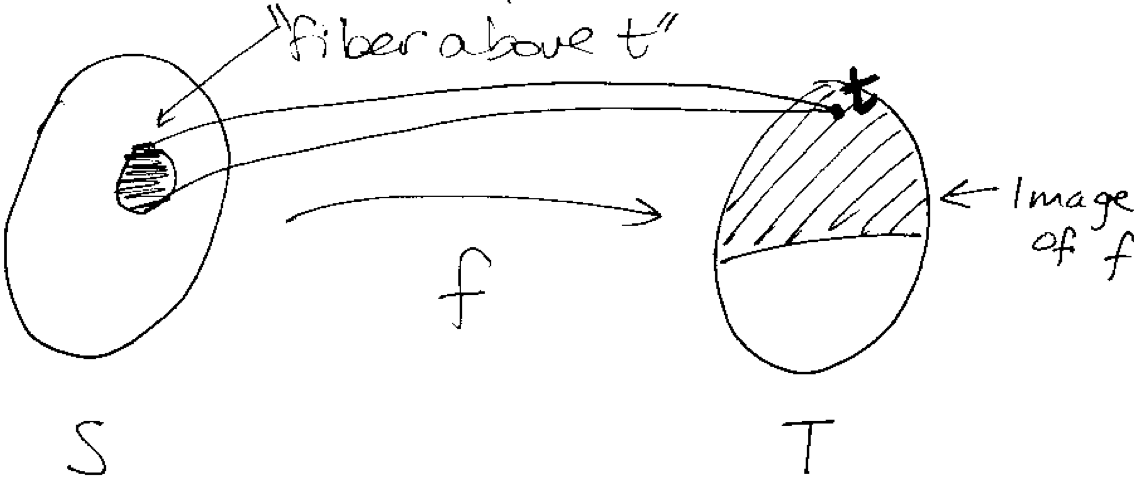
\includegraphics[scale=0.5]{images/fibre}
\caption{The \underline{fibre} above an equivalence class describes all elements which map to that equivalence class.}
\end{figure}

Suppose $S=\R$ and suppose $f (t) = \exp(2\pi i t)$. $T$ is the unit circle in $\C$. The fibre above $1$ or $f^{-1}(1)$ is clearly all integers. 

Suppose $\phi:G\to G'$ is a group homomorphism. Let $H \lhd G$ be the kernel of $\phi$. We get an equivalence relation on $G$ where $H$ is one of the equivalence classes of $G$. Any time we have a group homomorphism, we get a partition of $G$ into pieces where one of the partitions is the kernel of the homomorphism. This is the case because $H = \phi^{-1}(e')=\{a\in G:\phi(a)=\phi(e)=e'\}$. 
\begin{proposition} The other equivalence classes have the form $a H = \{a h : h \in H\}$ for some $a \in G$. \end{proposition}
\begin{proof}
Suppose $\phi(a)=\phi(b)\in G'$, i.e. $a\sim b$. Then $\phi(a^{-1}b) = e'$ so $a^{-1}b\in H$, i.e. $a^{-1}b=h$ so $b=ah$ for some $h\in H$. Conversely, any $b\in aH$ is equivalent to $a$ since $\phi(b)=\phi(ah)=\phi(a)\phi(h)=\phi(a)$ since $h$ is in the kernel.
\end{proof}

$aH$ is called a \underline{left coset} of $H$ in $G$.

The map $h\mapsto ah$ gives a bijection of sets $H\to a H$. In particular, $|H| = |aH|$ if $|H|$ is finite; so, for a group homomorphism, the equivalence classes are of the form $a(\ker \phi)$ and are of the same order. 
\begin{corollary} Assume $G$ is finite and $\phi : G\to G'$ is a homomorphism with kernel $H$. Then $|G| = |H|\cdot|\im\phi|$.\end{corollary}

This corollary is somewhat analogous to the following result in linear algebra. If $T:V\to W$ is a linear map, then $\dim V = \dim (\ker T) =\dim (\im T)$.

$|S_n| = n!$. For $n\geqslant 2$, $|A_n|=n!/2$.
\begin{proof}
$f:S_n\to \{\pm 1\}$ is a homomorphism (the sign map). $f$ is surjective for $n\geqslant 2$ with kernel $A_n$.
\end{proof}

More generally, let $H\subset G$. We define the left coset of $a\in G$ by $aH = \{ah:h\in H\}$. 
 \begin{proposition}
These subsets are disjoint and partition $G$. Furthermore, they each are in set-theoretic bijection with $H$.
\end{proposition}

Define the \underline{index of $H$} which may be infinite and denoted $[G:H]$ as the number of distinct left cosets, i.e. equivalence classes.
\begin{corollary}
If $G$ and $H$ are of finite order, then $|G| = |H| \cdot [G:H]$.
\end{corollary}

\underline{Lagrange's theorem} states that if $|G|$ is finite and $g\in G$, the order of $g$ divides $|G|$.
\begin{proof}
Let $H=\langle g\rangle = \{e,g,\hdots, g^{m-1}\}$, so $|H|=m$. Since $|H|\mid |G|$ by corollary 2.2, the result follows.
\end{proof}

Let $G$ be a finite group with $|G|=\textrm{some prime } p$. Then $g$ is cyclic generated by any $g\in G $ with $g\neq e$. Furthermore, the only subgroups of $G$ are $e$ and $G$.
\begin{proof}
Let $g\neq e\in G$. The order of $g$ divides $p$ and is not $1$. Since $p$ is prime, order of $g=p$, which says that $\langle g\rangle \subset G$ which both have order $p$. Therefore, they are equal.
\end{proof}

Can we show that this is a strong result by exhibiting a non-cyclic group of order $p^2$? Yes, the Klein four-group is of order $2^2$ and is not cyclic. Eventually, all groups of order $p^2$ are abelian.

A group $G$ is \underline{simple} if its only normal subgroups $H$ are $\{e\}$ and $G$. Examples:
\begin{enumerate}[label=(\roman*)]
\item Any $G$ of prime order (the only abelian simple groups).
\item $A_n$ for $n\geqslant 5$.
\item \underline{Feit-Thompson theorem:} (suggested by Richard Brauer) any finite, non-abelian, simple group has even order.
\end{enumerate}

Denote ``evens'' by $\overline{0}$ and ``odds'' by $\overline{1}$. Addition table:
$$
\begin{tabular}{ c|c|c } 

  ${+}$ & ${\overline{0}}$ &  ${\overline{1}}$   \\ 
\hline
 $\overline{0}$ & $\overline{0}$ &$\overline{1}$\\
 \hline
 $\overline{1}$ & $\overline{1}$ &$\overline{0}$\\
 
\end{tabular}
$$
Multiplication table: 
$$
\begin{tabular}{ c|c|c } 

  ${\times}$ & ${\overline{0}}$ &  ${\overline{1}}$   \\ 
  \hline
 $\overline{0}$ & $\overline{0}$ &$\overline{0}$\\
 \hline
 $\overline{1}$ & $\overline{0}$ &$\overline{1}$\\
 
\end{tabular}
$$
We want to generalize this from $2$ to ${n}$. 

Fix a positive integer $n$ and define an equivalence relation on $\Z$ by
$$
a\sim b \iff (a-b)\in n\Z
$$
This is clearly an equivalence relation as it satisfies all axioms. Notation for $a\sim b$:
$$
a\equiv b \pmod {n}
$$
It is said ``$a$ congruent to $b \mod n$''.

For $a\in \Z$, $\bar{a}$ denotes the equivalence class of $a$. 
$$
\bar{a} = a+n\Z= \{a + kn : k\in\Z\}
$$
$\bar{a}$ is a coset of $\Z$; $n\Z\subset \Z\implies a+n\Z$.

If $n=12$, $2\equiv 26 \pmod {12}\implies \bar{2}=\bar{26}$

There are $n$ distinct cosets of $n\Z $ (equivalence classes $\mod n$) which we can write out explicitly:
$$
\bar{0}, \bar{1}, \bar{2}, \hdots, \bar{n-1}
$$
This is the case because, due to the division algorithm, $a\in\Z\implies a =nq+r$ where  $q,r\in\Z$ and $0\leqslant r < n$; namely, $\bar{a}=\bar{r}$. $\bar{a}=\bar{b}$ and $0\leqslant a$, $b\leqslant n \implies 0\leqslant|a-b|\leqslant n-1$; $|b-a|\in n\Z \implies |a-b|=0\implies a=b$.

Notation for set of equivalence classes is $\Z/n\Z$ or simply $\Z/n$.

Consider the map (reduction $\mod n$) $${r} : \Z \to\Z/n\Z $$ where $a\mapsto \bar{a}$. We can do arithmetic in $\Z/n\Z $ by defining $\bar{a} +\bar{b} = \bar{a+b}$ and $\bar{a}\cdot{\bar{b}} = \bar{a\cdot b}$ which is well-defined.

$(\Z/n\Z,+)$ is a group:
\begin{enumerate}[label=(\roman*)]
\item Associative because $(\Z,+)$ is associative.
\item Identity $\bar{0}$.
\item Inverses $-\bar{a} =\bar{n-a}=\bar{-a}$.
\end{enumerate}

The set of cosets of $n\Z\subset{\Z}$ forms a group.

$\Z/n\Z$ is a cyclic group of order $n$ (generated by $\bar{1}$). Since all cyclic groups of order $n$ are isomorphic, we make two deductions.
\begin{enumerate}[label=(\roman*)]
\item There is always a cyclic group of order $n$.
\item All cyclic groups can be written in the form $\Z/n\Z$ for some $n$.
\end{enumerate}
When we use $+$ as the group operation, we write $g\cdot n$ rather than $g^n$.

Addition and multiplication on $\Z/n\Z$ distribute which is inherited from $\Z$.

Compute the last two digits of $2^{1000}$. All we have to do is compute $2^{1000}\pmod{100}$. We know that $2^{10} = 1024\equiv 24 \pmod{100}$. We know that $2^{20}=(2^{10})^2\equiv24^2\pmod{100} \equiv 576\pmod{100}  \equiv 76\pmod{100}$. We know that $76^2 = 5776 \equiv 76\pmod{100}$. By induction, $76^n\equiv 76\pmod{100}$. Therefore, $2^{1000} \equiv 76\pmod{100}$.

Is $(\Z/n\Z, \cdot)$ a group? $\bar{0}$ certainly cannot have an inverse. We do, however, have a subset of $\Z/n\Z$ that gives a group under multiplication:
$$
(\Z/n\Z)^\times = \{\bar{a} \in\Z/n\Z : \exists\ \bar{c} \in \Z/n\Z : \bar{a} \cdot \bar{c} = \bar{1}\}
$$

Review of $\gcd$: if $m,n \in \Z^\times$ then $\gcd({m,n}) =$ the largest positive integer which divides $m$ and $n$. It is the unique positive integer $d$ such that $d\mid m, n$ and if $e$ is another integer dividing $m$ and $n$, then $e\mid d$.
\begin{lemma}
$m\Z + n\Z = \{mr+ ns \mid r,s\in\Z\}=\gcd({m,n})\Z$.
\end{lemma}
\begin{proof}
$m\Z + n\Z$ is a subgroup of $\Z$ and so equals $d\Z$ for some positive integer $d$. Then $m\in m\Z+n\Z =d\Z\implies d\mid m$. Similarly, $d\mid n$. Furthermore, if $e\mid m, n$, then since $mr +ns = d\in d\Z$, $e$ must divide $d$.
\end{proof}
\begin{proposition}
$(\Z/n\Z)^\times = \{\bar{a}\in\Z/n\Z : \gcd(a,n)=1\}$.
\end{proposition} 
\begin{proof}
 Two possibilities:\begin{enumerate}[label=(\roman*)]
\item The righthand side is a subset of the lefthand side. If $\gcd(a,n)=1$, then by the lemma $a\Z+n\Z = \Z$. Thus, for every $r,s\in\Z$ such that $ar+ns=1$, $ar-1\in n\Z\implies\bar{a}\cdot\bar{r}=\bar{1}\implies\bar{a}\in(\Z/n\Z)^\times$.
\item The lefthand side is a subset of the righthand side. $\bar{a}\cdot\bar{c} = \bar{1}\implies ac-1=nb \implies 1 = ac-nb \in a \Z+n\Z=\gcd(a,n)\Z$.
\end{enumerate}
\end{proof}

An example of this is $(\Z/p\Z)^\times$, where evidently all numbers up to $p$ are coprime to $p$. More generally, $|(\Z/p^e\Z)^\times|=p^e-p^{e-1}$ since the only things not coprime to $p$ are its multiples.

If $G\lhd H$, then $G/H = \{\textrm{cosets of } H\subset G\}$. There is a natural homomorphism $f : G\to G/H$ with full image and kernel $H$.

It is a good exercise to prove that the surjective group homomorphism ${r} : \Z \to \Z/n\Z$ has kernel $n\Z\lhd \Z$.
\section{Quotient groups, vector spaces over finite fields}
Let us use $\Z/n\Z$ to denote a cyclic group of order $n$; it has a natural generator $\bar{1}$. 

When can we put a group structure on the set of cosets $\{aH\}$ for a subgroup $H\subset G$? Suppose $H = \ker f$ where $f:G\to G'$. The set of cosets $\{aH\}$ is the set of fibres in the map, which can be identified bijectively as the points $\bar{a}$ in the image---each coset corresponds to a point in the image. $\im f$ is a subgroup of $G'$. \textit{Par transport de structure}, we get a group structure on the set $G/H$ of cosets of the form $aH \cdot bH = ab\cdot H$ since $f$ is a homomorphism. This makes the map $\phi: G\to G/H$ where $a\mapsto aH$ a surjective group homomorphism. The identity of $G/H$ is $H$ and $(aH)^{-1}=a^{-1}H$

Let $H\subset G$ be any subgroup. $G/H=\{\textrm{cosets } aH\}$. Try to define  a group structure on $G/H$ by $aH\cdot bH=ab\cdot H$. Is this multiplication well-defined? i.e. if $aH=a'H$ and $bH=b'H$, is $(ab)H=(a'b')H$? Suppose $aHa^{-1}\neq H$, i.e. $aH\neq Ha$ for some $a\in G$. By this definition $(aH)(a^{-1}H)=eH=H$. But there exists some $h\in H$ such that $aha^{-1}\notin H$. We conclude the multiplication is not well-defined because $(ah)(a^{-1}e)\notin H$. The first example had $aHa^{-1}=H$ for all $a\in G$, so it was a normal subgroup. This is why the multiplication was well-defined.

So far, to answer our question is
\begin{enumerate}[label=(\roman*)]
\item Yes if $H=\ker (f:G\to G')$.
\item Not in general.
\end{enumerate}

Let us assume $H\lhd G$ so $aHa^{-1}=H$ for all $a\in G$, or $aH= Ha$. It does not have to commute, but for some $h,h'\in H$, $ah=h'a$. The ``na\"ive'' multiplication law of cosets is well-defined and defines a group structure on $G/H$. We have to calculate the set of all products $(aH) (bH )=\{ahbh'\in G : h,h'\in H\}$. We know that must be equal to $(Ha)(bH)$ which in turn is equal to $H(ab)H$ by associativity. Pushing on, that is equal to $(ab)HH=(ab)H$. It is well-defined. 

The answer to our question is yes $\iff H$ is normal.

We can then put a group structure on the set of all cosets $\{aH\}$ for a subgroup $H\subset G \iff H$ is normal. We also get a surjective group homomorphism 
$$
f: G\to G/H:a\mapsto aH
$$
with kernel $f^{-1}(eH)=H$.

\begin{corollary}
Every normal subgroup $H\lhd G$ is the kernel of a group homomorphism.
\end{corollary}
The \underline{isomorphism theorem} states that if $f:G\to G'$ is a surjective group homomorphism with kernel $H$, then $f$ induces an isomorphism of groups
$$
{\phi} : G/H\isom G'.
$$
In other words, you can take a surjective homomorphism and turn it into an isomorphism by going to the quotient group.
$\phi(aH)=f(a)$ by definition, and this equality is well-defined since $f(a)=f(a')$ for $a'\in aH$. This is certainly surjective. Also, $\ker \phi = \{e=eH\}$ (trivial). 

Construct a map $\pi :G\to G/H:a\mapsto aH$. The isomorphism theorem therefore says that any homomorphism factors through the quotient group:
$$
 \begin{tikzcd}[]
G \arrow[two heads]{dr}{\pi} \arrow{rr}{f}
    & & G'  \\
& G/H\arrow{ur}{\phi}  \end{tikzcd}
$$

A \underline{short exact sequence} of groups is a diagram of five groups, like so:
$$
 \begin{tikzcd}[]
1\arrow{r} & H\arrow{r}{f} & G\arrow{r}{g} & G' \arrow{r} & 1
\end{tikzcd},
$$
where $f$ and $g$ are group homomorphisms. $g(H)=\ker f$, $f$ is surjective (onto), and $g$ is injective (one-to-one). The isomorphism theorem says that $G'\simeq G/H$. $H$ is the ``kernel'' group and $G'$ is the ``image'' group.

Do not think that knowing $H$ and $G'$ implies knowledge of $G$.

Example: 
$$
 \begin{tikzcd}[]
1 \arrow{r} & A_3 \arrow[hookrightarrow]{r}\arrow[equal]{d} & S_3\arrow[equal, "\textbackslash" marking]{d} \arrow{r}{\textrm{sign}} & \langle \pm 1 \rangle\arrow[equal]{d} \arrow{r} & 1\\
1 \arrow{r} &\Z/3\Z\arrow{r} & \Z/6\Z \arrow{r} & \Z/2\Z\arrow{r} & 1
\end{tikzcd}
$$
$A_3$ is isomorphic to $\Z/3\Z$ and $\langle \pm 1 \rangle$ is isomorphic to $\Z/2\Z$. $S_3$ and $\Z/6\Z$ are not isomorphic since $S_3$ is non-abelian and $\Z/6\Z$ is abelian.

Suppose we have $G\supset K \lhd H$. Remember that $G\underset{f}{\twoheadrightarrow}G/H$ (the cosets of $H$) and $a\mapsto aH$.
We make the following statements:
\begin{enumerate}[label=(\roman*)]
\item $H$ is normal in $K$ since it is normal in $G$. We then have a group $K/H \subset G/H$, which is actually a subgroup of $G/H$. The cosets contained in $K$ are stable under multiplication as $K$ is stable under multiplication.
\item Conversely, any subgroup of $G$ containing $H$ corresponds to a subgroup of $G/H$, $\{aH\}$, in this manner:
$$
K = \bigcup_{\textrm{cosets}} aH = f^{-1}(\textrm{subgroup of }G/H)\in G
$$
\end{enumerate}

Suppose $G=\Z$ and $H=p\Z$.
\begin{proposition}
If $\Z\supset K\supset p\Z$ is a subgroup, then either $K=\Z$ or $K=p\Z$.
\end{proposition}
\begin{proof}
Such a $K$ gives a subgroup of the cyclic quotient group $\Z/p\Z$. A group of prime order has no non-trivial subgroups. This gives either 0 or $\Z/p\Z$. 0 corresponds to $p\Z$ because it is given by the union of cosets corresponding to the subgroup, and the only coset in that subgroup is $p\Z$. $p\Z$ corresponds to all of $\Z$ since that is produced from the union of all cosets corresponding to $p\Z$.
\end{proof}

Also, $p\Z$ is a ``maximal subgroup'' of $\Z$, meaning that it is a proper subgroup such that no proper subgroup $K$ contains it strictly. $p\Z$ being a maximal subgroup of $\Z$ comes from the proof of proposition 3.2.

A \underline{vector space} $V$ over $\R$ has the following properties.
\begin{enumerate}[label=(\roman*)]
\item An abelian group with operation $+$, identity $\mathbf{0}$, and inverse $-\bf{v}$.
\item Has scalar multiplication by $c\in\R$ ($\bf{v}\mapsto c\bf{v}$) satisfying
\begin{enumerate}[label=(\alph*)]
\item $0\cdot \bf{v} = \0$
\item $1\cdot \bf{v} = \bf{v}$
\item $(a\cdot b) \cdot\bf{v} = a\cdot (b\cdot \bf{v})$
\item $a\cdot (\bf{v} +\bf{w}) = a\cdot\bf{v} + a\cdot\bf{w}$
\item $(a+b)\cdot \bf{v} = a\cdot\bf{v} + b\cdot\bf{v}$
\end{enumerate}
\end{enumerate}
Examples of vector spaces include $\{0\}$, $\R$, and $\R^n$.

A \underline{field} $F$ is a set with two operations $+$ and $\times$ such that
\begin{enumerate}[label=(\roman*)]
\item It is an abelian group under $+$, 0 is the identity, $-a$ is inverse.
\item $F\setminus\{0\}=F^\times$ forms an abelian group under $\times$, 1 is the identity, $a^{-1}$ is inverse.
\end{enumerate}
We call $F'\subset F$ a subfield if it is a subgroup of a field closed under all criteria ($+$, $\times$, inverses, etc.). $\Q\subset\R\subset\C$ are all fields. Notice that $\Z$ is not a field.

The simplest field is $\Z/2\Z$. More generally, $\Z/p\Z$ is a field.\\\\
\dbend \ $\Z/n\Z$ for composite $n$ is not a field. \\\\
To show this, we must show that if $a\not\equiv 0 \pmod p$ then there is an integer $b$ such that $ab\equiv 1\pmod p$, i.e. $b\equiv a^{-1}\pmod p$.
\begin{proof}
Recall that $p\Z\subset \Z$ is a maximal subgroup. If $a\not\equiv 0 \pmod p$, then $a\notin p\Z$. Hence $p\Z+a\Z=\Z$ because $p\Z$ is maximal and $a$ is not in $p\Z$, meaning that we can write any integer as the sum of a multiple of $p$ and a multiple of $a$. This works for $1=mp+ba$ which implies that $1\equiv ba\pmod p$.
\end{proof}

$\Z/p\Z$ is evidently not a subfield of $\C$. A field $F$ must have a multiplicative identity: 1. $$\underbrace{1+1+\cdots+1}_{n \textrm{ times}}\in F.$$ In subfields of $\C$, these elements are distinct for every $n$. In $\Z/p\Z$, $$\underbrace{1+1+\cdots+1}_{p \textrm{ times}}=0,$$ which gives you $p$ in $\C$. 

Galois asked what the finite fields beyond $\Z/p\Z$ were. It turns out that there is a unique finite field of order $p^n$ up to isomorphism.

A vector space $V$ over a field $F$ is a set of vectors that
\begin{enumerate}[label=(\roman*)]
\item  is an abelian group under $+$ (identity $\0$).
\item has an operation (scalar product) $V\times F\to V : (\bf{v},\, c)\mapsto c\bf{v}$ where $0\cdot \bf{v} = \0$, $1\cdot \bf{v}=\bf{v}$, $(a\cdot b)\cdot \bf{v} = a\cdot(b\cdot\bf{v})$, $a\cdot(\bf{v}+\bf{w})=a\cdot\bf{v}+a\cdot\bf{w}$, etc.
\end{enumerate}

Examples of a vector space $V$ over a field $F$ include $V=\{\0\}$, $V=F$ (the field itself), $V=F^n=\{(a_1,\,\hdots,\,a_n) :a_i \in F\}$, and $$V=F[X]=\{\textrm{all polynomials $p(X)$ with coefficients} \in F\}.$$

$W\subset V$ is a vector subspace if it is a subgroup under $+$ and stable (closed) under scalar multiplication by $F$. For example, if $V=F^2$, a vector subspace of $V$ would be
$$
W=\{(a_1,\,a_2):a_1=ca_2,\,c\in F\}.
$$

$T:V\to W$ is a homomorphism (linear transformation/map) provided that $T(\bf{v}+\bf{w}) = T(\bf{v})+T( \bf{w})$ and $T(c\bf{v}) = cT(\bf{v})$. Just like with groups, a bijective homomorphism is an isomorphism. We define 
$$
\ker T = \{\bf{v}:T(\bf{v})=\0_W\} \subset V
$$
and
$$
\im T = \{T(\bf{v})\in W\}\subset W.
$$

If $V\subset W$, define $V/W$. It has vector space structure. $f:V\to V/W$ is a linear map with kernel $W$.

Normal subgroups are not an issue because we are dealing with abelian groups. We can transfer these notions from groups to vector spaces by assuming that the subgroup is stable under multiplication and the group homomorphism commutes with scalar multiplication.

$(\bf{v}_1,\hdots,\bf{v}_n)$ is an ordered finite set of vectors in a vector space, i.e. $V$. $\{\bf{v}_1,\hdots,\bf{v}_n\}$ with arbitrary order is a \underline{set of vectors} $S$. We have the concept of linear combinations:
$$
\bf{w}=a_1\bf{v}_1 + a_2\bf{v}_2+\cdots a_n\bf{v}_n,\, a_i\in F.
$$
The set of all such $\bf{w}$ is called the \underline{span} of $S$, which we denote $W$. $W$ is a subspace of $V$ since for $$\bf{w}'=b_1\bf{v}_1+\cdots+b_n\bf{v}_n,$$ we find that $$\bf{w}+\bf{w}'= (a_1+b_1)\bf{v}_1+\cdots+(a_n+b_n)\bf{v}_n $$ and $$c\bf{w} = (ca_1)\bf{v}_1+\cdots+(ca_n)\bf{v}_n.$$ It's clearly closed under addition and scalar multiplication. 

For convention, if $S=\emptyset$, then $\spn S = \{\0\}\subset V$.

$V$ is \underline{finite-dimensional} if there is a finite set $S$ of vectors in $V$ with $\spn S=V$.  For example, $V=F^n$ is finite-dimensional. If 
$$
\begin{aligned}
\bf{v}_1 &= (1,0,\hdots,0)\\\bf{v}_2 &= (0,1,\hdots,0)\\\vdots&\\\bf{v}_n &= (0,0,\hdots,1)
\end{aligned}
$$
then
$$
(a_1,\hdots,a_n)=\sum_i a_i\bf{v}_i.
$$
A non-example is $V=F[x]$. 

A set of vectors $\{\bf{v}_1,\hdots,\bf{v}_n\}$ is \underline{linearly independent} if the relation $$a_1\bf{v}_1+\cdots+a_n\bf{v}_n=\0$$ only holds when
$$
a_1=a_2=\cdots=a_n=0.
$$

If $V=\R^3$ and 
$$
\begin{aligned}
\bf{v}_1 &= (1,0,0),\\\bf{v}_2 &= (1,1,0), \textrm{ and}\\\bf{v}_3 &= (1,2,3),
\end{aligned}
$$
what is the span of $\{\bf{v}_1, \bf{v}_2\}$? It is of the form $\{\bf{v}=(a,b,0):a,b\in\R\}$. This would arise from the linear combination $b\bf{v}_2 + (a-b)\bf{v}_1$. These three vectors are also linearly independent. If
$$a_1\bf{v}_1+a_2\bf{v}_2+a_3\bf{v}_3=\0,$$
then $3a_3=0\implies a_3=0$ because the third component of $a_1$ and $a_2$ is 0. By similar logic we verify that $a_2=a_1=0$.

We say an ordered set $(\bf{v}_1,\hdots,\bf{v}_n)$ is a \underline{basis} of $V$ if it spans $V$ and is linearly independent in $V$. This means that every vector $\bf{w}\in V$ is uniquely expressed as a linear combination.

A basis gives rise to an isomorphism of vector spaces: $$f: V\isom F^n : \bf{w}\mapsto (a_1, \hdots, a_n).$$ This is clearly a homomorphism of vector spaces. It is onto since it spans $V$ and one-to-one since it is linearly independent in $V$.

\begin{theorem}
If $S = \{\bf{v}_1,\hdots,\bf{v}_n\}$ is a finite set that spans $V$, a subset of $S$ gives a basis for $V$.
\end{theorem}
\begin{proof}
If the elements of $S$ are linearly independent, we are done. If not, we have a relation
$$
a_1\bf{v}_1+\cdots+a_n\bf{v}_n=\0
$$
with some $a_i\ne 0$. Suppose we can reorder $S$ so that $a_n\ne 0$. Rearranging, 
$$
a_n\bf{v}_n=-(a_1\bf{v}_1+\cdots+a_{n-1}\bf{v}_{n-1}) \in V.
$$
$a_n^{-1}$ exists since we're in a field. Multiplying by $a_n^{-1}$,
$$
\bf{v}_n = -\frac{1}{a_n} (a_1\bf{v}_1+\cdots+a_{n-1}\bf{v}_{n-1}).
$$
Hence, $\spn S = \spn \{\bf{v}_1,\hdots,\bf{v}_{n-1}\}$, which is $V$. This shows that we can pull a vector out of $S$ and have the same span. If the new set is linearly independent, we're done. If not, repeat until the resulting set is linearly independent.
\end{proof}

\begin{theorem}
If $L$ is a linearly independent set of vectors in $V$, it can be extended to form a basis in $V$.
\end{theorem}
\begin{proof}
If $L$ spans $V$, we're done. If not, let $S$ be a finite set spanning $V$. There must be a $\bf{v}\in S$ such that $\bf{v} \notin \spn L$. We claim that $L\cup \{\bf{v}\}=L'$ is linearly independent. To see why, suppose $L=\{\bf{w}_1,\hdots,\bf{w}_n\}$ and $$
\sum a_i\bf{w}_i + b\bf{v}=\0.
$$
Then $b=0$, or else $$\bf{v}=-\frac{1}{b}\left(\sum a_i\bf{w}_i \right)$$ is in the span of $L$. Hence, $\sum a_i\bf{w}_i=\0$, implying that all $a_i=0$ as $L$ is linearly independent. If $L'$ spans, we're done. If not, there is some $\bf{v}'\in S$ not in the span of $L'$. We continue to apply this adjoining of vectors in $S$ until we achieve a set spanning $V$.
\end{proof}

\begin{theorem}
If $S=\{\bf{v}_1,\hdots,\bf{v}_n\}$ spans $V$ and $L=\{\bf{w}_1,\hdots,\bf{w}_m\}$ is linearly independent in $V$, then $n\geqslant m$.
\end{theorem}
\begin{proof}
Since $S$ spans, we may write each element in $L$
$$
\bf{w}_j = \sum_i a_{ij}\bf{v}_i.
$$
We will now try to make a non-trivial linear relation on $\bf{w}_j$: 
$$
\begin{aligned}
\0&=\sum_j c_j\bf{w}_j\\
&= \sum_j c_j \left(\sum_i a_{ij}\bf{v}_i\right)\\
&= \sum_i\left(\sum_j a_{ij}c_j\right)\bf{v}_i.
\end{aligned}
$$
If we can arrange that $\sum_j a_{ij}c_j=\0$ for all $i$ with some $c_j\ne 0$, then $\bf{w}_j$ could not be linearly independent. All $i$s make up $n$ linear equations with $m$ unknowns. If $m>n$ (more unknowns $c_j$ than equations indexed by $i$), we can find a non-trivial solution. But if $m>n$, that contradicts $L$ being linearly independent. If $m$ cannot be greater than $n$, $n\geqslant m$.
\end{proof}

\begin{corollary}
All bases of $V$ have the same number of elements denoted $\dim V$.
\end{corollary}
\begin{proof}
Let $B$ and $B'$ be two bases. Since $B$ spans and $B'$ is linearly independent, $\#B\geqslant\# B'$. Since $B'$ spans and $B$ is linearly independent, $\#B'\geqslant\# B$. By the squeeze theorem, $\#B=\#B'$.
\end{proof}
\begin{corollary}
All spanning sets $S$ have $\#S\geqslant \dim V$.
\end{corollary}
\begin{corollary}
All linearly independent sets $L$ have $\#L\leqslant \dim V$.
\end{corollary}

Note that $\dim\{\0\}=0$ and $\dim F^n =n$.

\begin{proposition}Suppose $W\subset V$ and $\{\bf{w}_1,\hdots,\bf{w}_m\}$ is a basis for $W$. Then we may extend this to a basis for $V$.\end{proposition}\begin{proof} The basis is linearly independent in $V$ and so it can be extended to a basis.\end{proof}%QED

$W\subset V$ gives a homomorphism $f: V\to V/W$ (quotient vector space). In this map, the first $m$ vectors go to $\0$ since they are in the kernel. In fact, 
$$
(f(\bf{v}_{m+1}),\hdots,f(\bf{v}_n))
$$
gives a basis for $V/W$. Consequently, $\dim V = \dim W + \dim (V/W)$. $$W'=\spn\{\bf{v}_{m+1},\hdots,\bf{v}_n\}$$ is a subspace of $V$ mapping isomorphically to $V/W$.\\\\
\dbend \ In group theory, we cannot think of the quotient group being inside of the group. \\\\Take the following example:
$$
\Z/2\Z\simeq 2\Z/4\Z =H \subset \Z/4\Z =G
$$
There does not exist $H'\supset G$ mapping isomorphically to $G/H$ because $H'$ would have to be of order 2, but the only subgroup of order 2 is $H$. If we take the image of $H$ in the map to $G/H$, we get 0.


\section{Abstract linear operators, the characteristic polynomial}

Let $W$ be the subspace of $V$ spanned by $\{\bf{v}_1,\,\hdots,\, \bf{v}_n\}$ and let $W'$ be the subspace spanned by $\{\bf{v}_{n+1},\, \hdots,\, \bf{v}_m\}$ (the set of vectors appended to $W$ to form a basis of $V$). Then $W\cap W' = \{\0\}$ and we have a linear isomorphism
$$
W\times W' = \{(w,w') : w\in W,\, w'\in W'\} \isom V : (w,w')\mapsto w+w'.
$$
This is a homomorphism from the vector space structure on the product (component-wise and scalar multiplication). It is surjective because $\{\bf{v}_1,\,\hdots,\, \bf{v}_m\}$ spans. It is injective because 
$$
w_1 + w_1' = w_2 + w_2' \implies w_1 - w_2\, (\in W) = w_2' - w_1'\, (\in W')
$$ 
and this common vector is in $W\cap W'$, which means the vector is $\0$. Also, $w_1 = w_2$ and $w_1' = w_2'$. This fact implies that the way we wrote these vectors as sums in the first place was unique.

If $W\subset V$ then there is another $W'\subset V$ s.t. there exists this composite map:
$$
W' \hookrightarrow V \twoheadrightarrow V/W
$$ 
where
$$
w' \mapsto w'\mapsto w'+W.
$$
The surjection is the \underline{canonical quotient map}. This composite map is an isomorphism. We take a basis of $W$ and extend it to a basis of $V$. Let $W' =\spn\{\bf{v}_{n+1},\,\hdots,\, \bf{v}_m\}$ (using the notations we have used heretofore). Using these $W$ and $W'$ the previous assertion that this composition is an isomorphism can be verified.

From these last two arguments, we get for $W\subset V$ that 
$$
V \isom W \times V/W.
$$
Observe that 
$$
\dim V = \dim W + \dim (V/W).
$$

If $f: V \to U$ is a linear transformation, then
$$
V \isom \ker f \times \im f
$$
and by the previous argument
$$
\dim V =  \dim(\ker f) +\dim (\im f).
$$
\begin{proof}
The isomorphism theorem for groups implies a sort of isomorphism theorem for vector spaces that incorporates the linear structure. Given a linear transformation $f:V\to U$, the map $$\bar{f}: V/\ker f \to \im f$$ is a well-defined linear isomorphism.
\end{proof}

We now analyze a general problem for groups. Given $f : G\to G'$, trying to find the kernel and image of $f$ is generally difficult. We can solve this problem in the case of vector spaces using bases, matrices, and matrix algorithms. Let us look at some correspondences.
%https://www.khanacademy.org/math/linear-algebra/alternate-bases/change-of-basis/v/lin-alg-transformation-matrix-with-respect-to-a-basis
Firstly, suppose $V$ is an $n$-dimensional vector space over $F$. There is a bijective correspondence between ordered bases of $V$ and linear isomorphisms $F^n \isom V$. Suppose we have a basis $B = (\bf{v}_1,\,\hdots,\, \bf{v}_n)$. There is an isomorphism 
$$
\rho_B : F^n\to V : \left(\begin{matrix}a_{1} \\\vdots \\a_{n}\end{matrix}\right) \mapsto a_1\bf{v}_1 + \cdots + a_n\bf{v}_n. 
$$
How do we go in the other direction? Suppose we have a linear isomorphism $F^n\to V$. What basis corresponds to it? Precisely
$$
\left(\rho \left(\begin{matrix}1\\0\\\vdots\\0\end{matrix}\right), \,\rho \left(\begin{matrix}0\\1\\\vdots\\0\end{matrix}\right),\, \hdots ,\,\rho \left(\begin{matrix}0\\0\\\vdots\\1\end{matrix}\right)\right) \mapsfrom \rho.
$$

Secondly, linear transformations $F^n\to F^m$ correspond to $M_{m\times n} (F)$ matrices.

Given these two correspondences and a linear transformation $f :V \to V'$ with dimensions $n$ and $m$ and bases $B$ and $B'$ respectively, we have the matrix of $f$ with respect to $B$ and $B'$ defined as 
$$
[f]_B^{B'} = [\rho_{B'}^{-1} f\rho_B].
$$
Explicitly, if $B=(\bf{v}_1,\,\hdots,\, \bf{v}_n)$ and $B'=(\bf{w}_1,\,\hdots,\, \bf{w}_m)$ then 
$$
f(\bf{v}_j) = \sum_i a_{ij}\bf{w}_i
$$
and
$$
[f]_B^{B'} = (a_{ij}).
$$
These notions allow us to say that $\Hom(V,\,V')$ (linear transformations from $V$ to $V'$) given a choice of bases is isomorphic to $M_{m\times n}(F)$. $\Hom(V,\,V')$ has a vector space structure. We find that
$$
[c_1f_1+c_2f_2]_B^{B'} = c_1[f_1]_B^{B'} + c_2[f_2]_B^{B'}
$$
and if $f:V\to V'$ and $g:V'\to V''$, equipped with bases $B$, $B'$, and $B''$, composition is preserved:
$$
[g\circ f]_B^{B''} = [g]_{B'}^{B''} [f]_B^{B'}.
$$

Let us introduce the notion of change of basis. There can be multiple bases for a given vector space. Suppose $V$ and $V'$ are each equipped with two bases.
\begin{align*}
[f]_{B_2}^{B_2'} &=  [\rho_{B_2'}^{-1} f\rho_{B_2}]\\
			 &=  [\rho_{B_2'}^{-1}\rho_{B_1'}\rho_{B_1'}^{-1}f\rho_{B_1}\rho_{B_1}^{-1}\rho_{B_2}]\\
			 &=  [\rho_{B_2'}^{-1}\rho_{B_1'}][\rho_{B_1'}^{-1}f\rho_{B_1}][\rho_{B_1}^{-1}\rho_{B_2}]\\
			 &=  [\rho_{B_2'}^{-1}\rho_{B_1'}][f]_{B_1}^{B_1'}[\rho_{B_1}^{-1}\rho_{B_2}]
\end{align*}
We call something of the form $[\rho_{B_1}^{-1} \rho_{B_2}]$ a \underline{change of basis matrix}. If $V=V'$,
\begin{align*}
[f]_{B_2}^{B_2} &=  [\rho_{B_1}^{-1}\rho_{B_2}]^{-1}[f]_{B_1}^{B_1}[\rho_{B_1}^{-1}\rho_{B_2}]\\
			&=  P^{-1}[f]_{B_1}^{B_1}P
\end{align*}
$P$ is the change of basis matrix (conjugacy). 

To calculate, if $B_1 = (\bf{v}_1,\,\hdots,\, \bf{v}_n)$ and $B_2 = (\bf{w}_1,\,\hdots,\, \bf{w}_n)$, 
$$
[\rho_{B_1}^{-1}\rho_{B_2}] = (c_{ij}),\  \bf{w}_j = \sum_i c_{ij}\bf{v}_i.
$$

Suppose $V$ is a vector space. We define
\begin{align*}
 \GL(V)  	&= \{\textrm{linear isomorphisms }V\to V\} \subset \Aut(V)\\
		&= \{\textrm{invertible linear transformations }V\to V\} \\
		&= \Hom(V,\,V)^\times.
\end{align*}
Given a basis $B$ of $V$, we can rewrite this isomorphically as the set of invertible matrices in $M_{m\times n}(F)$, $\GL_n(F)$.

Suppose $V$ and $W$ are finite-dimensional vector spaces over a field $F$ and $T:V\to W$ is a linear operator; namely, 
$$
T(\bf{v} + \bf w ) = T(\bf v) + T(\bf w)
$$  
and 
$$
T(c\bf v) = cT(\bf v).
$$
As a famous example, 
$$
T = d/dx : V\to W
$$
is a linear operator. Another example is the total derivative of $F:\R^n \to \R^m$ at a point.

What is $\ker(d/dx)$ when $F = \Z/p\Z$? it always contains the constants; but, if $n\geqslant p$ (where $n$ is the polynomial's degree) we have $x^p$ in the kernel. Let us recall that 
$$
\ker T = \{ \bf v \in V : T(\bf v) = \0 \} \subset V
$$
and
$$
\im T = \{  \bf w \in W : \bf w = T(\bf v)\} \subset W.
$$
Note that
$$
\dim V = \dim (\ker T) + \dim (\im T).
$$
\begin{proof}
Let $\{\bf v_1,\,\hdots,\, \bf v_k\}$ be a basis of $\ker T$. From linear independence in $V$, we extend this basis to a basis $\{\bf v_1,\,\hdots,\, \bf v_k,\,\bf v_{k+1},\,\hdots,\,\bf v_n\}$ of $V$. Then $\{\bf w_i = T(\bf v_{k+i})\}$ is a basis for $\im T$ for $i = 1,\hdots,n-k$. They span since 
\begin{align*}
\bf w = T(\bf v)  &= T\left(\sum_{i=1}^ka_i\bf v_i + \sum_{i=k+1}^nb_i\bf v_i\right)\\
			&= \sum_{i=1}^ka_iT(\bf v_i) + \sum_{i=k+1}^nb_iT(\bf v_i)\\
			&= \sum b_iT(\bf v_i)\\
			&= \sum_{i=1}^{n-k} b_i\bf w_i.
\end{align*}
Assume that there is a relation
$$
\sum b_i\bf w_i = \0_W.
$$
Consider the vector
$$
\bf{v}_0 = \sum_{i=1}^{n-k}b_i\bf v_{i+k} \in V.
$$
We claim that $T(\bf v_0) = \0_W$, which means that this vector is in the kernel of $T$. So
\begin{align*}
\bf v_0 = \sum_{i=1}^k a_i\bf v_i = \sum_{i=1}^{n-k} b_i\bf v_{i+k}.
\end{align*}
Hence
\begin{align*}
 \sum_{i=1}^k a_i\bf v_i - \sum_{i=1}^{n-k} b_i\bf v_{i+k} = \0_W,
\end{align*}
which is a linear relation on the basis of $V$. So all $a_i = 0$ and all $b_i=0$, which means that each $\bf w_i$ is linearly independent. 
\end{proof}
\begin{corollary}
If $V$ is finite-dimensional and $W\subset V$ then $\dim W + \dim(V/W) = \dim V$.
\end{corollary}
\begin{proof}
There is a homomorphism $T:V\to V/W:\bf v\mapsto \bf v + W$ that is surjective with kernel $W$.
\end{proof}

Introducing some formal nomenclature, $\dim(\ker T)$ is called the nullity of $T$ and $\dim(\im T)$ is called the rank of $T$.

If $V$ and $W$ have bases $\{\bf v_1,\hdots,\bf v_n\}$ and $\{\bf w_1,\hdots,\bf w_m\}$, there is an isomorphism $V\to F^n$ where $\bf v \mapsto (a_1,\hdots, a_n)$ and similarly for $W$. What does $T:V\to W$ look like once these isomorphisms have been chosen? Consider this diagram:
$$
 \begin{tikzcd}[]
V\arrow{r}{\sim} \arrow{d}{T} & F^n\arrow[dashed]{d} \\
W\arrow{r}{\sim} & F^m
\end{tikzcd}
$$
Each 
$$
T(\bf v_i) = \sum_{i=1}^ma_{ij}\bf w_i
$$
for $j=1,\hdots, n$ and $a_{ij}$ in $F$, which is determined by $T$ and the choice of basis. Conversely, the scalars $\{a_{ij}\}$ determine $T$. Write 
$$
\bf v = \sum _{j=1}^m x_j\bf v_j.
$$
Then
\begin{align*}
T(\bf v) &= \sum_{j=1}^n x_j\left(\sum_{i=1}^m a_{ij}\bf{w}_i\right)\\
	    &= \sum_{i=1}^m y_i\bf{w}_i.
\end{align*}
Precisely, define $A$ as an $m\times n$ matrix $(a_{ij})$ where the image of  $T\bf v_j$ is in the $j$th column. We translate this to say, for a column vector $Y$,
$$
\left(\begin{matrix}y_1\\\vdots\\y_m\end{matrix}\right) = Y = AX = A \left(\begin{matrix}x_1\\\vdots\\x_n\end{matrix}\right)
$$
Therefore, the diagram above fills in
$$
\begin{tikzcd}
V\arrow{r}{\sim} \arrow{d}{T} & F^n\arrow[]{d} \\
W\arrow{r}{\sim} & F^m
\end{tikzcd}
$$
such that the map from $F^n$ to $F^m$ is completed by left multiplication by a matrix $A$. $F^n$ and $F^m$ are thought of as column vectors. 

Take $T: V\to W$ where $V$ has a basis $\{\bf v_1,\bf v_2\}$ and $W$ has a basis $\{\bf w_1,\bf w_2\}$; also, $$T\bf{v}_1 = 2\bf w_1 \textrm{ and } T\bf{v}_2 = 3\bf w_1 + 4\bf w_2.$$ The resulting matrix is as follows, where the first column contains the coordinates $T\bf v_1$ and the second contains the coordinates of $T\bf v_2$:
$$
A = \begin{pmatrix} 2 & 3 \\ 0 & 4\end{pmatrix}.
$$
Suppose $\bf{v} = 7\bf v_1 + 8 \bf v_2 \in V$ and you wanted to see what the linear operator did to it. You could substitute the $\bf v$ terms in terms of $\bf w$; however, you could use the matrix multiplication demonstrated above:
$$
A\left(\begin{matrix}7\\8\end{matrix}\right) = \left(\begin{matrix}38\\32\end{matrix}\right) = 38 \bf w_1 + 32 \bf w_2
$$

If $T: V\to V$, we call $T$ an \underline{endomorphism}: a homomorphism from a vector space to itself. We get a square matrix $A$ of $T$ with respect to a given basis of $V$. If 
$$
\begin{tikzcd}
V\arrow{r}{T} & V\arrow{r}{S} & V,
\end{tikzcd}
$$
where $A$ and $B$ are separate matrices representing $T$ and $S$, what is the matrix of $S\circ T : V\to V$? You get $B\cdot A$ (matrix multiplication). In fact, matrix multiplication arose from the composition of linear operators. Why matrix multiplication is associative is why the composition of linear operators is associative.

\begin{proposition}
The following statements are equivalent for $T: V\to V$:
\begin{enumerate}[label=(\roman*)]
\item $T$ is an isomorphism (an automorphism) of vector spaces.
\item $\ker T = 0$.
\item $\im T = V$.
\item If the matrix $A$ of $T$ with respect to a basis of $V$ is $A$ then $A$ is invertible as an $m\times n$ matrix.
\item $\det A$ is non-zero in $F$.
\end{enumerate} 
\end{proposition}
Note that 
$$
\{T: V\to V \textrm{ isomorphisms}\} = \GL(V) \simeq \GL_n(F)
$$
under multiplication with a choice of basis. 

If $F = \Z/2$, what is $\GL_2(F)$? There are sixteen choices of two-by-two matrices, but only six are invertible. In fact, 
$$
\GL_2(F) \simeq S_3.
$$
How can we see this fact? $F^2$ is the set of four vectors $\{(0,0),\, (0,1),\, (1,0),\, (1,1)\}$. Any linear operator takes $(0,0)$ to itself. The remaining three vectors can be permuted arbitrarily. 

If $A$ is the matrix of a transformation $T:V\to V$ with respect to a basis $\{\bf v_1,\hdots, \bf v_n\}$, what is the matrix with respect to a different basis $\{\bf v'_1,\hdots, \bf v'_n\}$, $A'$?
$$
A' = PAP^{-1} 
$$
where $P$ is the invertible $n\times n $ matrix giving the change of basis. $P$ is called the conjugate matrix. 

The advantage of the $(V, T)$ point of view over the $(F^n, A)$ point of view is by choosing a convenient basis, we can get a simpler form for our operator.

From the previous proposition, there is a basis of $V$ and a basis of $W$ such that the matrix of $T$ is a zero matrix with an $r\times r$ identity matrix in the top-left, where $r$ is the rank of $T$:
$$
\begin{pmatrix} I_r & \\  & \end{pmatrix}.
$$
We choose the basis of $V$ to be a concatenation of elements mapping to the basis of the image and elements in the kernel. We map the first elements of $V$ with $T$ to the basis of $W$ and choose the remaining elements of the basis arbitrarily. These choices lead to the matrix described above. 

If $T:V\to V$, can we find a good basis such that the matrix $A$ of $T$ is in simple form? An \underline{invariant subspace} $W\subset V$ is a subspace satisfying $T(W)\subset W$. If we have such a subspace, $A$ has a special form where you start off with the first $n$ basis vectors in $W$; the coordinates when transformed under $T$ lie in $W$, so we obtain a square matrix in the top left of the matrix and zeros below:
$$
A = \begin{pmatrix} a & b\\  &d \end{pmatrix}.
$$
Now suppose the invariant subspace has an invariant complement $W'\subset V$, which means that
$$
V = W\oplus W',
$$
$\bf v = \bf w + \bf w'$ uniquely, and $T(W')\subset W'$. If we have such a situation, we can adjoin the bases of $W$ and $W'$ to get a full basis in $V$. Therefore,
$$
A = \begin{pmatrix} a & \\  &d \end{pmatrix}
$$
where $a$ contains the basis vectors of $W$ and $d$ contains the basis vectors of $W'$. If $W$ is one-dimensional (it contains multiples of a fixed vector $\bf w$ in some field) and invariant, then $T\bf w = c\bf w$. We say that $\bf w$ is an eigenvector and $c$ is an eigenvalue. If there is a basis $\{\bf v_1,\hdots, \bf v_n\}$ of $V$ consisting of eigenvectors with $T\bf{v}_i = c_i\bf v_i$, then
$$
A = \begin{pmatrix} c_1 & && \\ &c_2 && \\ &&\ddots & \\ &&&c_n \end{pmatrix}. 
$$

We cannot always write $A$ in this diagonal form; we cannot always determine a basis of eigenvectors. Consider in $\R^2$ the transformation rotating a vector $\bf v$ by an angle $\theta$ to $T\bf v$. If we take the basis with respect to the standard basis of $\R^2$, we get the matrix of $T$ to be 
$$
A = \begin{pmatrix} \cos \theta & -\sin \theta\\ \sin \theta &\cos \theta \end{pmatrix}
$$
There are no eigenvectors $\bf v \neq \0$ in $\R^2$ for $T$ if $\theta \neq 0,\pi$.

Now consider $T:F^2\to F^2$, for which $T(\bf e_1) = \bf e_1$ (an eigenvector with eigenvalue $c=1$) and $T(\bf e_2) = \bf e_1+\bf e_2$. The matrix of $T$ is
$$
A = \begin{pmatrix} 1 & 1\\ 0 &1 \end{pmatrix},
$$
which you should note has the same form as a matrix above. We claim that there is no basis of eigenvectors; i.e. there is no complement $W'$ that is $T$-invariant for $W=F\bf e_1$. Let us suppose otherwise. Let $\bf v = a\bf e_1 + b\bf e_2$. We get 
\begin{align*}
T\bf v &= a\bf e_1 +b(\bf e_1+\bf  e_2)\\
          &= (a+b)\bf e_1 + b\bf e_2.
\end{align*}
Could the previous be equal to $c\bf v$? We know that $c\bf v = ca\bf e_1 + cb\bf e_2$; this implies that $ca = a+b$ and $cb = b$. If $b$ is non-zero, we get $c=1$. If $c=1$, $a = a+b$, so $b=0$. Here we reach a contradiction. The only way that we can obtain a second eigenvector is if $b=0$, and so $c=1$. Therefore, the only eigenvectors are of the form $\bf v = a\bf e_1\in W$, which we already knew.

Now suppose we are given $T$; what are the possible eigenvalues $c$? If $T\bf w = c\bf w$, then
$$
(T - c I)\bf w = \0,
$$
i.e. $\bf w \in \ker(T - c\cdot I)$ and $T - c I$ is not invertible. Conversely, if $T-cI$ has a kernel (or is not invertible) then $c$ is an eigenvalue for $T$. So, the set of eigenvalues is
$$
\{c\in F : T-cI \textrm{ not invertible}\}
$$
or 
$$
\{c\in F : \det(A-cI)=0\}
$$
where $A$ is the matrix of $T$ with respect to some basis. 

Consider the determinant 
\begin{align*}
&\det(tI - A)\\
=&\,\det \begin{pmatrix} t-a_{11} &\cdots&\cdots& -a_{1n}\\ -a_{21}&t-a_{22} &\cdots&\vdots \\ \vdots&\vdots&\ddots &\vdots \\ -a_{n1}&\cdots&\cdots&t-a_{nn} \end{pmatrix}\\
=&\, t^n - (a_{11} + \cdots + a_{nn})t^{n-1} +\cdots + (-1)^n\det A.
\end{align*}
This is a polynomial in $t$ of degree $n$ with coefficients in the field $F$. It is called the \underline{characteristic polynomial of $T$}. Observe that the characteristic polynomial $f(t)$ depends only on $T$, not on the basis of $V$ used to obtain the matrix $A$ to calculate it. If we used a different basis, we get $A^* = PAP^{-1}$. Applying the previous determinant,
\begin{align*}
f^*(t) &= \det (tI-A^*)\\
&= \det (tI - PAP^{-1})\\
&= \det(P(tI-A)P^{-1})\\
&= \det P \cdot f(t) \cdot \det(P^{-1})\\
&= \det P \cdot (\det P)^{-1} \cdot f(t)\\
&= f(t).
\end{align*}
A miracle! Also, the roots of the characteristic polynomial are the eigenvalues.
\begin{lemma}
If $f(t)$ has degree $n$ over a field $F$ then it has at most $n$ distinct roots $c$ in $F$.
\end{lemma}
\begin{proof}
We use a division algorithm. Write $f(t) = (t-c)g(t)+d$, where $d$ is in $F$ and $\deg(g(t)) = n-1$. If $f(c)=0$, then $d=0$, so $f(t)=(t-c)g(t)$. If $c'$ is another root with $c'\neq c$, then $g(c') = 0$. The proof follows from induction on $\deg g$.
\end{proof}
So a transformation $T$ of $V$ has at most $\dim V$ distinct eigenvalues.

In the case of the rotation transformation before, 
$$
f(t) = t^2 - (2\cos\theta)t + 1.
$$
We know that $|2\cos\theta|<2$ for $\theta \neq 0,\pi$, so $f$ has no real roots. 

For a general $2\times 2$ matrix
$$
A = \begin{pmatrix} a & b\\ c &d \end{pmatrix},
$$
we have
$$
f(t) = t^2 - (a+d)t + (ad - bc).
$$
We call $a_{11} + \cdots + a_{nn}$ the \underline{trace of $A$}. So,
$$
f(t) = t^2 - (\tr A)t + \det A.
$$

If we were asked what the eigenvalues of 
$$
A = \begin{pmatrix} 3 & 2\\ 1 &4\end{pmatrix}
$$
were, we would get 
\begin{align*}
f(t) &= t^2 - 7t + 10\\
     &=(t-5)(t-2).
\end{align*}
Therefore, $c = 5,2$ are eigenvalues; namely, there is a $\bf v_1$ such that $T\bf v_1 = 5 \bf v_1 $ and a $\bf v_2$ such that $T\bf v_2=2\bf v_2$. We get a basis of eigenvectors here if $2\neq 5$ in $F$. 

If
$$
f(t) = (t-c_1)(t-c_2)\cdots(t-c_n)
$$
for distinct $c_i$, we get a basis of eigenvectors. 

$T:V\to V$ gives a vector in $\Hom(V,V)$: an $F$--vector space of dimension $n^2$. In this vector space we have $\{I, T, T^2, \hdots, T^{n^2}\}$. There are $n^2 + 1$ vectors here; so, there must be a linear relation 
$$
a_0I + a_1T + \cdots a_{n^2}T^{n^2} = 0
$$
in $\Hom(V,V)$. Therefore, $T$ satisfies a polynomial of degree less than or equal to $n^2$ with coefficients in $F$.

\begin{theorem}
(Cayley-Hamilton) $T$ always satisfies its own characteristic polynomial (with $\deg n$).
\end{theorem}
This theorem is easily verified for $2\times 2$ matrices. 
\begin{proof}
(where $f(t)=(t-c_1)\cdots(t-c_n)$ for distinct $c_i$) We have
$$
A = \left(\begin{array}{cccc} c_1 & && \\ &c_2 && \\ &&\ddots & \\ &&&c_n \end{array}\right).
$$
Now consider 
$$
f(A) = (A-c_1I)\cdots(A-c_nI).
$$
$A-c_i$ is diagonal with a $0$ in the $i$th place so $f(A)=0$.
\end{proof}

We will now explore some interesting subgroups of the general linear group:
$$
\SO_n(F)\lhd_2 \O_n(F) \subset\GL_n(F).
$$
When $F=\R$, they are related to Euclidean geometry. To define these subgroups, we take $V=F^n$ and put an additional structure on it; namely, we equip $V$ with an inner product (or bilinear form):
$$
\langle\bf v, \bf w\rangle = v_1w_1 + \cdots + v_nw_n.
$$
From here, we define
$$
\O_n(F) = \{A\in \GL_n(F) : \langle A\bf v, A\bf w\rangle= \langle\bf v,\bf w\rangle\},
$$
the \underline{orthogonal group}, which we can verify is a subgroup of $\GL_n(F)$.

A matrix $A\in \O_n(F)$ has each its $n$th column corresponding to what $A$ does to $\bf e_n$. You turn a matrix into an operator by seeing what it does to the standard basis. Observe that
$$
\langle \bf e_i, \bf e_j \rangle = \delta_{ij}.
$$
This fact implies that $\langle A\bf e_i, A\bf e_j \rangle $ is the inner product of the $i$th and $j$th columns. This implication is stunningly equivalent to saying that
$$
\t{A} \cdot A = I.
$$
Therefore, we can also define
$$
\O_n(F) = \{A\in \GL_n(F) : \t{A}=A^{-1}\}.
$$
Let us rewrite
$$
\langle\bf v,\bf w\rangle = \t{\bf v}\cdot \bf w.
$$
So, 
$$
\langle A\bf v,A\bf w\rangle = \t{\bf v}\cdot(\t{A}\cdot A)\cdot\bf w.
$$
By using properties of the transpose and determinant, we have
$$
\det A = \pm 1.
$$
Now we can define
$$
\SO_n(F) = \{A\in \O_n(F) : \det A = 1\},
$$
the \underline{special orthogonal group}, which is a group of index $2$; thinking about the determinant as a homomorphism
$$
\O_n(F) \underset{\det}{\longrightarrow}\langle\pm 1\rangle
$$
allows us to think of $\SO_n(F)$ as the kernel of this homomorphism.

We claim that the permutation matrices are in $\O_n(F)$ which gives an injective homomorphism
$$
f : S_n\hookrightarrow \O_n(F) : A_n \hookrightarrow \SO_n(F)
$$
where $1\neq -1$ in $F$.

Now take $F=\R$. Note that 
$$
\langle\bf v, \bf v\rangle = \sum_i a_i^2 \geqslant 0
$$
and $\langle\bf v, \bf v\rangle = 0$ iff $\bf v=\0$. We define the Euclidean norm or length of $\bf v$ as
$$
|\bf v| = \sqrt{\langle\bf v, \bf v\rangle}. 
$$
We also have the Cauchy-Schwartz inequality:
$$
-1 \leqslant \frac{\langle\bf v, \bf w\rangle}{|\bf v||\bf w|}\leqslant +1 
$$
for $\bf v, \bf w \neq \0$.The term bounded between $\pm 1$ is $\cos \theta$ where $\theta \in [0, \pi]$ is the angle between $\bf v$ and $\bf w$.

The group $\O_n(\R)$ acts linearly on $\R^n$ and preserves lengths and angles. (It preserves the notions of Euclidean geometry.)

\section{Orthogonal groups, groups of rigid motions, their finite subgroups}
In any field $F$, if $\bf v$ where $\langle\bf v,\bf v\rangle$ is an eigenvector for $A\in\O_n(F)$ with eigenvalue $\lambda$, then $\lambda^2 = 1$; so, $\lambda = \pm 1$. We can see this fact because
$$
\langle \bf v,\bf v\rangle = \langle A\bf v,A\bf v\rangle = \langle \lambda\bf v,\lambda\bf v\rangle = \lambda^2\langle \bf v,\bf v\rangle.
$$
We then divide by $\langle\bf v,\bf v\rangle$ to get $\lambda^2 = 1$.

What do transformations $A$ in $\SO(2)$ over $\R$ look like? Note that $|\bf e_1| = |\bf e_2| = 1$ and $\langle \bf e_1,\bf e_2\rangle = 0$; they are orthogonal. $A\bf e_1$ and $A\bf e_2$ must lie on the unit circle since they are of length 1. We can write $A\bf e_1$ as $(\cos\theta, \sin\theta)$; since $A\bf e_2$ is orthogonal to $A\bf e_1$, we write $A\bf e_2$ as either $(-\sin\theta, \cos\theta)$ or $(\sin\theta, -\cos\theta)$. Since $\det A = 1$, 
$$
A = \left(\begin{array}{cc} \cos\theta & -\sin\theta\\ \sin\theta & \cos\theta\end{array}\right);
$$ 
so, $A\bf e_2 = (-\sin\theta, \cos\theta)$, which is in the upper left quadrant. We write $A$ as $\rot\theta$, which is the most general transformation in $\SO(2)$.
Observe that 
$$
\rot\theta \circ \rot\phi = \rot(\theta + \phi).
$$
There is a isomorphism of abelian groups
$$
f : \SO(2) \isom \{z\in \C^\times : |z| =1\} : A =\rot \theta \mapsto z = e^{i\theta} = f(\bf e_1).
$$
\dbend \ $\O(2)$ is not abelian. \\

What are the transformations $A\in \O(2)-\SO(2)$ (where $\det A = -1$)? Each such $A$ has two orthogonal eigenvectors $\bf v_1, \bf v_2$ where 
$$
A\bf v_1 = \bf v_1 \textrm{ and } A\bf v_2 = -\bf v_2 
$$
and 
$$
A = \left(\begin{array}{cc} 1 &\\ & -1\end{array}\right) 
$$
with respect to $\bf v_1, \bf v_2$.
\begin{proof}
The characteristic polynomial of $A$ is $x^2 -\tr(A)x-1 = 0$. We claim that both roots of this polynomial are real; if not, the two roots are conjugate in $\C$. But $\det A = z\bar{z}\geqslant 0$. But $\det A = -1$, meaning that both roots $\lambda_1$ and $\lambda_2$ are real. Moreover,
$$
\lambda_1\lambda_2 = -1.
$$
Every root of the characteristic polynomial gives an eigenvalue of $A$; so, $\lambda_1 = \pm 1$ and $\lambda_2 = -\lambda_1$. A simple check shows that $\bf v_1$ and $\bf v_2$ are orthogonal.
\end{proof}

$A$ looks like the reflection of $\bf{v}_2$ by the line $\R\bf v_1$ where $\bf v_1$ is the vector with eigenvalue $1$. Notice that 
$$
\refl \bf v_1 \circ \refl \bf v_2 = \rot\theta.
$$
We can show that reflections do not commute.
\begin{theorem}
(Euler) Any $A$ in $\SO(3)$ has an eigenvalue of $+1$ such that there is a $\bf v\in\R^3$ for which $A\bf v = \bf v$. In Euler's terms, any motion preserving $S^2 \subset \R^3$ with determinant $+1$ has an axis of rotation.
\end{theorem}
\begin{proof}
The characteristic polynomial has degree $3$, so $3$ roots in $\C$. One possibility is that all roots are real, and a second is that one root is real and the other two are complex conjugates; by the intermediate value theorem, these are the only two possibilities. We know that the product of the roots is $1$ since we are in $\SO(3)$. If all roots are real, at least one root must be $+1$; if one root is real, it must be $+1$ since the product of the complex conjugates is $+1$.
\end{proof}
Geometrically in $\R^3$, the transformation preserves the unit sphere. Eigenvalues stay fixed. We claim that $A$ preserves the plane orthogonal to the eigenvector $\bf v$. If $\langle\bf v, \bf w\rangle = 0$, $\langle A\bf v, A\bf w\rangle = 0$, which means that
$$
\langle\bf v,A \bf w\rangle = 0.
$$
If a vector is on this orthogonal plane, it remains on the plane after the transformation. The matrix of $A$ has its first column as $\bf v$ and its second two form an orthogonal basis of the plane orthogonal to $\bf v$:
$$
A = \left(\begin{array}{ccc} 1 &0&0\\ 0& &\\0&&\end{array}\right),
$$
where the missing $2\times 2$ matrix is an orthogonal transformation spanned by $\{\bf e_1,\bf e_2\}$ with determinant $+1$; therefore, it is in $\SO(2)$. So, this inner matrix is just some $\rot \theta$. The transformation rotates all planes perpendicular to $\bf v$ by $\theta$. 

All motions $\R^n\to\R^n$ preserving distance $d(\bf v,\bf w)=|\bf v-\bf w|$ between two points from a group $G$ of \underline{rigid motions}. 

We claim that if $m$ is a rigid motion and $m(\0)=\0$ then $m$ is a linear transformation in $\O(n)$.
\begin{proof}
\textit{That $\langle m(\bf v), m(\bf w) \rangle = \langle \bf v, \bf w \rangle$.} We know that 
$$
|\bf v - \bf w|^2 = \langle \bf v-\bf w, \bf v -\bf w \rangle = |\bf v|^2 + |\bf w|^2 - 2 \langle \bf v, \bf w \rangle,
$$
which are preserved by $m$ by definition.
\end{proof}
We have not shown that $m$ is linear. We do find that 
$$
\O(n)\subset G.
$$
Another subgroup of $G$ involves translating by a fixed vector $\bf b$:
$$
t_{\bf b}(\bf v) = \bf v + \bf b
$$
where 
$$
t_{\bf b} \circ t_{\bf b'} = t_{\bf b+\bf b'}.
$$
It is isomorphic to $\R^n$ under addition.

We can therefore show that if $G$ is the group of rigid motions
$$
G = \O(n) \cdot \R^n,
$$
in the sense that any rigid motion can be written uniquely as the composition of a translation and a rotation. $\R^n$ is normal in $G$.

Let us claim that any element in the group of motions $G$ can be written uniquely as a product of something in $\R^n \simeq t_\bf{b}$ and something in the subgroup of motions which preserve 0, $G_0$:
$$
G = \R^n \cdot G_0.
$$
We have also claimed that
$$
G_0 \simeq \O(n).
$$
The inner product is preserved, but we need linearity. To get linearity, let $\bf e_1,\hdots,\bf e_n$ be the standard basis of $\R^n$. Remember the inner product properties of standard bases. Then $m(\bf e_1),\hdots,m(\bf e_n)$ is another orthonormal basis. Let $A$ be the element in $\O(n)$ with column vectors $m(\bf e_1),\hdots,m(\bf e_n)$. Note that $\t(A)\cdot A = I$. We claim that $m=A$ as a transformation of $\R^n$.
\begin{proof}
Consider the motion $m\circ A^{-1} = m'\in G_0$. For all $i$
$$
m'(\bf e_i) = \bf e_i.
$$
We claim $m'(\bf v) = \bf v$ for $\bf v \in \R^n$, i.e. $A=m $ on $\R^n$. The $i$th coordinate of $m'(\bf v)$ is $$\langle m'(\bf v), \bf e_i \rangle = \langle m'(\bf v), m'(\bf e_i)\rangle=\langle \bf v, \bf e_i\rangle=v_i.$$ This shows that $m'$ fixes $\bf v$.
\end{proof}

We have now identified the elements in $G_0$ bijectively with the orthogonal transformations:
$$
m(\bf v) = A(\bf v) + \bf b
$$
where $\bf b\in \R^n, A \in \O(n)$ (a translation and an orthogonal matrix). This is the only way we can get a transformation of $n$-dimensional space that preserves distance. What do products look like in $G$?
\begin{align*}
(\bf b, A) \cdot (\bf b', A') (\bf v)	&= (\bf b, A)(A' \bf v + \bf b')\\
						&= A(A'\bf v + \bf b')+\bf b\\
						&= AA'(\bf v) + (A(\bf b') + \bf b)\\
						&= (\bf b + A(\bf b'), AA')(\bf v)
\end{align*}
This product is not commutative. 

The map 
$$
f : G\to \O(n) : (\bf b, A)\mapsto A
$$
is a surjective group homomorphism with kernel $\R^n$. $\R^n$ is normal in $G$ and $\O(n)$ is a subgroup isomorphic to the quotient group.

Consider $n=2$:
$$
G = \R^2 \cdot\O(2)
$$
and 
$$
G_0 = \O(2) = \SO(2) \cup \SO(2)r_\ell
$$
where $r_\ell$ is the set of order $2$ reflections about a line through the origin.
\begin{align*}
r_\ell\circ \rot(\theta)\circ r_\ell^{-1}	&=r_\ell\circ \rot(\theta)\circ r_\ell \\
							&= \rot\theta ' 
\end{align*}
for some $\theta'$. We know it is a rotation since the composition of the determinants gives us $+1$. Looking at where a point on the reflection line goes after this composition, we find that $\theta' = -\theta$. Now we have a nice description of $G_0 = \O(2)$ in terms of $\SO(2)$ and any fixed reflection,

We have the map
$$
G =\R^2 \cdot \O(2) \to \O(2)\underset{\det}{\to} \{\pm 1\}
$$ 
which determines orientation. Any $g\in G$ is one of four types:
\begin{enumerate}[label=(\alph*)]
\item $\det g = +1$: orientation-preserving and of the form $t_\bf b \circ\rot\theta$.
\begin{enumerate}[label=(\roman*)]
\item Translations fixing no points or all points.
\item Translations fixing a single point $\bf p$ and consisting of rotations around $\bf p$.
\end{enumerate}
\item $\det g=-1$: orientation-reversing and of the form $t_\bf b \circ\rot\theta\circ\refl\ell$.
\begin{enumerate}[label=(\roman*)]
\setcounter{enumii}{2}
\item Reflection of the form $\refl (\ell)$ in a line fixing it pointwise.
\item Glide reflection $\refl(\ell)(\bf v) + \bf b$ that fixes $\ell$.
\end{enumerate}
\end{enumerate}
Let's look in greater detail:
\begin{enumerate}[label=(\roman*)]
\item Where $\theta = 0$
\item Where $\theta \neq 0$ and assuming $\bf b \neq \0$. How do we find the fixed point with these values given? We take $\bf b$ and take the unique line orthogonal to it. We then make a line $\theta/2$ north of the orthogonal line and one  $\theta/2$ south of the line to get a sector of $\theta$. We can therefore find a vector of magnitude $\bf b$ going from the one line segment to the other, giving us the only fixed point $\bf p$. 
\end{enumerate}

Let's now study the finite subgroups $\Gamma$ of $G=\R^2\cdot \O(2)$. $\Gamma$ contains no translations. 
\begin{theorem}
Any finite $\Gamma$ fixes a point $\bf p \in \R^2$, i.e. $\gamma(\bf p) = \bf p$ for all $\gamma \in \Gamma$.
\end{theorem}
We determine an abstract recipe to determine the fixed point $\bf p$. Let $\bf s\in \R^2$ be any vector. Consider the vectors $\{\gamma(\bf s) : \gamma \in \Gamma\}$. Let $n = \#\Gamma$ and  
$$
\bf p = \frac{1}{n} \sum_{\gamma\in\Gamma} \gamma(\bf s).
$$
We claim that $\bf p$ is fixed, i.e. if $g\in G$, 
$$
g(\bf p) = \frac{1}{n}\sum g\gamma(\bf s).
$$
It is simple to check for $g$ a translation (divided by $n$) and $g\in \O(2)$ (linear maps) to verify for all $g\in G$ that $g(\bf p) = \bf p$.

If $\bf p = \0$, then $\Gamma \subset \O(2)$. In general,
$$
\Gamma \subset G_\bf p \subset G
$$
where
$$
G_\bf p = \{g : g(\bf p) = \bf p\} = t_\bf p\circ G_0 \circ t_\bf p^{-1}.
$$
So $t_\bf p^{-1} \Gamma t_\bf p\subset G_0 = \O(2)$, which we will notate $\Gamma^*$, a finite group isomorphic to $\Gamma$. We have proven that the finite subgroups of this complicated group $G$ are isomorphic to the finite subgroups of $\O(2)$.

Let's classify the finite $\Gamma \subset \O(2)$:
\begin{enumerate}[label=(\roman*)]
\item $\Gamma\subset \SO(2)$ ($\det \Gamma = +1$).
\item $\Gamma \cap \SO(2) = \Gamma_+ $ has index $2$ in $\Gamma$ (normal subgroup) ($\det \Gamma = \pm 1$).
\end{enumerate}
In the first case, every $\gamma = \rot \theta \in [0,2\pi]$. Let $\theta>0$ be the smallest angle of rotation for $\gamma\in \Gamma$. Then $\Gamma$ is a cyclic group generated by this element. If $|\Gamma| = n$,  $\theta = 2\pi/n$. Every $\Gamma$ is cyclic and all orders can occur. 

In the second case, $\Gamma_+$ is cyclic of some order $n$. In particular for a reflection $r$, $\Gamma_+$ is
$$
\langle \rot(2\pi/n), r \rangle.
$$
$r$ has order $2$ since $C_n \subset \Gamma$ of order $2n$ is of index $2$ and the rotation has order $n$. These groups are called \underline{dihedral groups} of order $2n$; they are non-abelian for $n\geqslant 3$.

So, if $\Gamma \subset G$ is a finite subgroup, then $\Gamma$ fixes $\bf p \in \R^n$. Therefore, it is conjugate to a finite subgroup of $\Gamma \subset \O(n)=G_0$ fixing $\0$. 
{
Restating earlier remarks, if $\Gamma\subset \O(2)$ and $\Gamma_+ = \{ \gamma\in\Gamma : \det \gamma = 1 \}$, we have two cases. If $\Gamma=\Gamma_+$, it is cyclic of order $n\geqslant 1$ generated by $\rot \theta$ for the smallest angle $\theta$. If $\Gamma \rhd \Gamma_+$, it is dihedral of order $2n$ and so $\Gamma_+$ is cyclic of order $n$. For a reflection $r\in \Gamma - \Gamma_+$, 
$$
r\rot(\theta)r^{-1} = \rot(\theta)^{-1}
$$
where $r^2 = 1$. 

Regular $n$-gons are preserved by these groups. Let's consider a regular hexagon, giving us the case for $n=6$. Think of the action of the cyclic group of order $6$ rotating each vertex by $\pi/3$. This is the smallest $\theta$ since rotating by $\theta$ $6$ times gives you the identity. We also have the dihedral group of order $12$ acting on the hexagon; in addition to the rotations from $\Gamma_+ = \langle \rot (\pi/3)\rangle$, we also have reflections. There are six such reflections, three reflecting about a line intersecting two vertices, and three reflecting about a line intersecting two edges. Here we have two conjugacy classes. For the triangle, reflections only go through one vertex and one edge. For odd $n$, reflections, or elements in $\Gamma-\Gamma_+$ are all conjugate; for even $n$, they form two conjugacy classes. Note that
$$
D_6 \simeq S_3
$$
and $D_4$ is isomorphic to the Klein four-group. Dihedral groups of order $6$ and above are non-abelian. In general, 
$$
D_{2n} \hookrightarrow S_n.
$$

More generally, we want to classify the \underline{discrete subgroups} $\Gamma\subset G$. For $G=\R^n\cdot\O(n)$, discrete means that $\Gamma$ does not contain arbitrarily small rotations or translations. i.e. there is an $\varepsilon > 0$ such that if $t_\bf b \in \Gamma$, $|\bf b| \geqslant \varepsilon$, and if $\rot \theta \in \Gamma$, $|\theta| \geqslant \varepsilon$. Thus, two finite subgroups are necessarily discrete, but the converse is false. 

Take $\Gamma \subset G = \R^n \cdot \O(n)$. Let $\bf b \neq \0\in\R^n$ and let 
$$
\Gamma = \textrm{cyclic group generated by } t_\bf b.
$$
This is an infinite discrete subgroup.

Let's classify discrete subgroups of $G= \R^2\cdot \O(2)$. Let $\Gamma$ be a discrete subgroup of $G$. Consider 
$$
L = \Gamma \cap \R^2 = \{t_\bf b \in\Gamma\}.
$$
and the image $\bar{\Gamma} = \Gamma/L$ of $G$ in $\O(2) = G/\R^2$. What are the possibilities for $L$? Firstly, $L = \{0\}$ when $\Gamma$ is finite. Secondly, $L = \Z\bf b$ for $\bf b \neq \0 \in \R^2$. Thirdly, $L = \Z\bf a + \Z\bf b$ where $\bf a $ and $\bf b$ form an $\R^2$ basis; in this case we call $L$ a \underline{lattice}.

Observe that if $\bf b,\bf b'\in L$, then $\bf b-\bf b'\in L$ and so $|\bf b -\bf b'| \geqslant \varepsilon$ for some fixed $\varepsilon$, i.e. vectors can't be too close to each other. Assume $L\neq 0$. In case two, all vectors in $L$ lie on a fixed line $\ell \in\R^2$. Let $\bf b$ be the closest vector in $L$ to the origin. Then $L = \Z\bf b$. Suppose $\bf b' =  n\bf b + r_0\bf b\in L$ for $n\in \Z$ and $0\leqslant r_0\leqslant1$. If $r_0\neq0$, then $r_0\bf b\in L$ and $|r_0\bf b| < |\bf b|$, and so $r_0=0$. 

In case three, not all $\bf b\in L$ lie on a line, i.e. $L$ contains a basis of $\R^2$. Take basis $\langle\bf a,\bf b\rangle$ where $\bf b$ is the shortest vector in $L$ on $\R\bf b$ and the same for $\bf a$.

\begin{lemma}
If $S$ is a bounded subset of $\R^2$, $S\cap L$ is finite. 
\end{lemma}
\begin{proof}
Suppose it is infinite. We can therefore choose a convergent subsequence since it is bounded. We reach a contradiction since no sequence of elements in $L$ is Cauchy. 
\end{proof}
Consider the parallelogram $P$ spanned by $\bf a $ and $\bf b$. There are a finite number of points inside $P\cap L$. Suppose $\bf b'$ is the vector closest to $\bf a$. Replace $\bf b\in L$ by $\bf b'$ if $\bf b$ wasn't the closest. The new parallelogram has the point $\bf b$ closest to $\bf a$. We now claim that $L = \Z\bf a = \Z\bf b$.
\begin{proof}
Any $\bf v\in \R^2$ is of the form $\bf v = r\bf a + s\bf b$ for real $r, s$. We can now write
$$
\bf v = (n\bf a + r_0\bf a) + (m\bf b + s_0 \bf b)
$$
for $m,n\in \Z$ and $0\leqslant r_0,s_0\leqslant1$. So $r_0\bf a + s_0\bf b \in L$. Such a vector would be in the parallelogram, but we determined that the parallelogram was empty. Therefore, $r_0,s_0=0$ and $\bf v \in \Z\bf a + \Z\bf b$. 
\end{proof}
Now consider the image of $\bar{\Gamma}$ of $\Gamma$ in $\O(2)$.
\begin{lemma}
$\bar \Gamma$ preserves the subgroup $L\subset \O(2)$.
\end{lemma}
\begin{proof}
Let $\bf b \in L$, i.e. $t_\bf b\in \Gamma$. Say $\bar\gamma \in \bar\Gamma$, and lift it to an element $\gamma \in \Gamma$. Consider $\gamma t_\bf b\gamma^{-1}\in \Gamma$. This is a translation by $\bar \gamma (\bf b)$, which is $t_{\bar \gamma(\bf b)}$. This means that $\bar\gamma(\bf b) \in L.$
\end{proof}
If $L=\{0\}$, $\bar\Gamma=C_n, D_{2n}$ for $n\geqslant 1$. Any such $\bar\Gamma$ is possible. Suppose we're in case three where $L=\Z\bf a+\Z\bf b$. Then $\bar\Gamma = C_n, D_{2n}$ with $n=1,2,3,4,6$ so $|\bar\Gamma| \leqslant 12$.
\begin{proof}
Let $A\in \bar \Gamma$ be a rotation. Consider the characteristic polynomial of $A$: $x^2 - \tr(A)x + 1.$
If we have a rotation by $\theta = e^{2\pi/n}$ giving a complex number $z$, then $\tr A = z + \bar z$.
Let $t = \tr A$. 
$$
t^2 - 4 \leqslant 0
$$
because the roots of the polynomial are two complex conjugates. Because $A$ stabilizes the lattice $L$, $\tr A\in \Z$ because matrix of $A$ with respect to the basis has integer entries. From these conditions, $\tr A$ can only be $\pm 2$ (order $3$ or $6$), $\pm 1$ (order $1$ or $2$), and $0$ (order $4$).
\end{proof}

\section{Isometrics of plane figures, group actions, the class equation}
So, if $L=\{0\}$, $\Gamma=\bar{\Gamma} = C_n \textrm{ or } D_{2n}$ for $n\geqslant 1$. If $L=\Z\bf a$ then $\bar\Gamma = C_1, C_2, D_2, \textrm{ or } D_4$, the Klein four-group. Take the line generated by $\bf a$. If $\gamma\in\bar\Gamma$, $\gamma(\bf a) = \pm \bf a$ as in $\Z\bf a$ and it is the same length as $\bf a$. If $\gamma\in\SO(2)$ then $\gamma = I$ or $-I$. If $L =\Z\bf a +\Z\bf b$ then  $\bar\Gamma = C_n, D_{2n}$ with $n=1,2,3,4,6$.
\begin{proof}
If $\gamma\in\bar\Gamma$ is a rotation by $\theta$, the characteristic polynomial of $\gamma$ is 
$$
f(X) = X^2 - 2\cos(\theta)X + 1.
$$
$|\cos\theta|\leqslant 2$. Since the matrix of $\gamma$ with respect to $\bf a$ and $\bf b$ contains integers, its trace is an integer. $2\cos\theta$ is an integer between $-2$ and $2$, and for $\theta = 2\pi/n$, $n$ could only be the five aforementioned numbers.
\end{proof}
What is the classification of lattices $L=\Z\bf a+\Z\bf b$ in $\R^2$? Changing $L$ to $\gamma L$ for $\gamma\in \O(2)$ just conjugates $\bar\Gamma=\Aut L$ by $\gamma$. Changing $L$ to $c\cdot L$ for $c\in\R^\times$ doesn't change $\bar\Gamma$. 
$L$ up to action of $\O(2)$ and $\R^\times$ on $\R^2$: we can assume shortest $\bf a$ has length one (the $\R_+^\times$ action. We can rotate $\bf a$ so that it is 1 (the $\SO(2)$ action). What about the second basis vector $\bf b$? We know that $|\bf b| \geqslant 1$. We can replace $\bf b$ by $-\bf b$ so that the $y$-coordinate is positive. Replace $\bf b$ by $\bf b + m\bf a$ so that the $x$-coordinate is between $-1/2$ and $1/2$. We can conclude that 
$$
L \simeq L_\bf b =\Z +\Z\bf b
$$ 
for $\bf b$ in the right half of the shaded region shown in figure $2$.
\begin{figure}
\centering
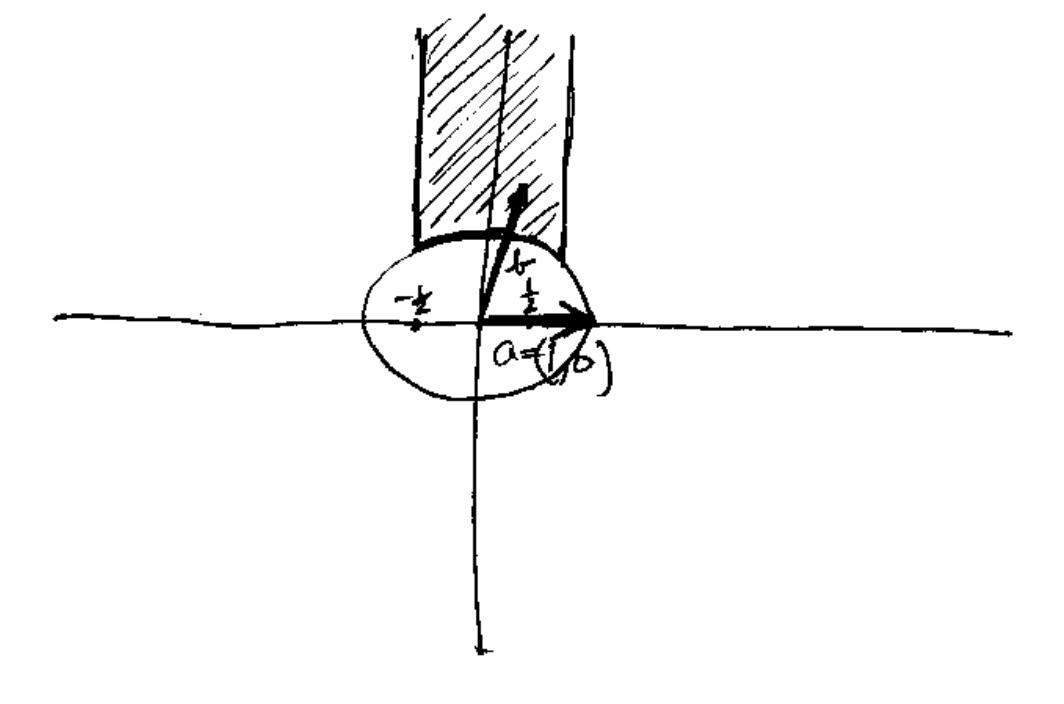
\includegraphics[scale=0.5]{images/lattice_bases}
\caption{$L\simeq \Z+\Z\bf b$ for $\bf b$ in the right half of the shaded region.}
\end{figure}

If $\bf b$ is the vector emerging from a $\pi/3$ rotation with $x$-coordinate $1/2$, we get an interesting lattice: the hexagonal lattice. There are six vectors around the origin that are the same length as $\bf a$. If you put a circle of radius $1/2$ at each of these points so that adjacent circles are tangent to each other, you get the best packing of two-dimensional space with circles. 

If $\bf b$ in strictly inside this region, the only possibilities for $\bar\Gamma$ are $1$ or $C_2=-I$.

If $\bf b \perp \bf a$, $\bar\Gamma = 1,C_2,D_2, \textrm{ or }D_4$. In the square lattice where $|\bf b| = 1$, $\bar\Gamma$ is one of $1,C_2,C_4,D_4,$ or $D_8$. In the hexagonal lattice, $\bar\Gamma = 1,C_2,C_3,C_6, D_6,$ or $D_{12}$.

A major question in modern mathematics is classifying lattices in $n$-space up to scaling and $\O(n)$. We have for $n\leqslant 8$, but no further.

We have been discussing group actions with the group of motions on $\R^2$. We can generalize this idea to a group $G$ and a set $S$. A group action on a set is a mapping 
$$
G\times S \to S : (g,s)\mapsto g(s).
$$
We need $e(s)=s$ for all $s\in S$ and associativity:
$$
gh(s) = g(h(s)).
$$

For an $s\in S$, we define the \underline{orbit of $s$} as
$$
O_s = \{g\cdot s : g\in G\}
$$
and the \underline{stabilizer of $s$} as
$$
G_s = \{g\in G: g \cdot s = s\}.
$$
We know that $O_\0 =\R^2$ and $G_\0 = \O(2)$. If $\ell$ is a line then $O_\ell$ is $S$: any line. If $\triangle $ is a triangle, $O_\triangle$ is not all triangles, but triangles congruent to $\triangle$. If $O_s =S$, $G$ acts \underline{transitively} on $S$.

The model case of a transitive $G$-action: if we have an arbitrary group $G$, $H$ any subgroup of $G$, and $G=G/H=\{aH:a\in G\}$. The $G$-action is by left translation:
$$
g(aH) = gaH.
$$
This action is transitive since $a(H) = aH$. The stabilizer $G_H $ is $H$. $G_{aH}$ is $\{g:gaH=aH\}$, which you can determine is $aHa^{-1}$.

More generally, if $G$ acts transitively on $S$ and $g(s)=s'$ then $G_{s'}  = gG_sG^{-1}$. So, all stabilizers are conjugate. In fact, the general transitive action is no more general than the coset action because if $G$ acts transitively on $S$ and $s\in S$ has stabilizer $G_s$, then there is a bijection of $G$-sets 
$$
G/G_s \isom S: g\mapsto g(s)
$$ 
that is well-defined as it only depends on the coset $G/G_s$. 
Transitive actions of $G$ are the same as conjugacy classes of subgroups of $G$. If $G$ and $S$ are finite, then
$$
\#G = \#S \cdot \#G_s. 
$$
As an example, if $G$ acts on $S=G$ by conjugation, $$s\mapsto gsg^{-1},$$ the orbits are the conjugacy classes and the stabilizer is the centralizer of $s$.

Remember that we have 
$$
G/G_s \isom O_s : gG_s \mapsto g(s).
$$
Suppose $G$ acts on $S$, both finite-ordered with orbits $O_{s_1},\hdots,O_{s_n}$. Then 
$$
|S| = |O_{s_1}| + \cdots + |O_{s_n}|
$$
and therefore
\begin{align*}
|S| 	&= |G/G_{s_1}| + \cdots + |G/G_{s_n}|\\
	&= |G| \sum_i \frac{1}{|G_{s_i}|}.
\end{align*}
% The order of G/N, by definition the number of elements, is equal to |G : N|, the index of N in G. If G is finite, the index is also equal to the order of G divided by the order of N. The set G/N may be finite, although both G and N are infinite (en.wikipedia.org/wiki/Quotient_group).
Suppose we have a finite group $G$ with two subgroups $H$ and $K$ and their intersection $H\cap K$. 
\begin{proposition}
$|G :K| \geqslant |H : H\cap K|$.
\end{proposition}
\begin{proof}
Let $G=G/K$. $|S| = |G:K|$. $G$ acts transitively on $S$. We can restrict the action of $G$ on $S$ to the subgroup $H$. This $H$-action is a union of $H$ orbits. Consider the orbit of the coset $eK$ under the action of $H$:  
$$
O_s \simeq H/H_s = \{h\in H : hK=K\} = H\cap K.
$$
\end{proof}
$G$ acts transitively on $S=G$ by left multiplication:
$$
g(s) = g\cdot s\textrm{ and } O_e = G.
$$
There is a more interesting action of $G$ on itself by conjugation:
$$
g(s) = gsg^{-1}.
$$
It is easy to verify that 
$$
gh(s) = g(h(s)).
$$
In this case, 
$$
O_e = \{e\} \textrm{ and } G_e = G.
$$
Unless $G$ is trivial, this action is not transitive.

So, by definition, the orbit of $s$
$$
O_s = \textrm{conjugacy class of } s.
$$
Also, 
\begin{align*}
|G| 	&= \sum_{\textrm{conjugacy classes}} |O_s|\\
	&= \sum_{\substack{\textrm{conjugacy classes}\\\textrm{of } G}} \frac{|G|}{|Z_s|}
\end{align*}
where 
$$
Z_s = \{g\in G : gs = sg\}
$$
is the stabilizer. 
% https://brilliant.org/wiki/conjugacy-classes/
The above equality is called the \underline{class equation}. If $G$ is abelian, every orbit has one element where 
$$
G_s = G.
$$

Suppose $G=S_3$. Its first conjugacy class is that containing the identity. The second contains three elements of order $2$: the transpositions. The last contains two elements of order three.

For conjugation action, when is $|O_s|=1$? Equivalently, when is $G_s=G$? When $s\in Z$.

\begin{theorem}
If $|G|=p^n$ with $p$ prime, $Z\neq \{e\}$.
\end{theorem}
\begin{proof}
$|G|/|Z_s| = p^k$ with $0\leqslant k\leqslant n$. So, all are divisible by $p$ except when $k=0$ and $|O_s|=1$. Therefore $\#Z$ is divisible by $p$ and thus not equal to $1$.
\end{proof}

If $G$ is of prime power order and $Z$ is the centre, then 
$$
G_1 = G/Z
$$
has prime power order $<\#G$ with centre $Z_1$. We then take 
$$
G_2 = G_1/Z_1,
$$
and continue this process until we break down to the trivial group. $G$ is not simple unless $|G| = p$. 

Burnside: If $|G| = p^nq^m$ then $G$ is not simple. 

Let us look into finite subgroups $G \subset \SO(3)$ preserving the regular solids in $\R^3$. Elements in $\SO(3)$ preserve the points on the unit sphere $S^2$. Every $g\in G$ is a rotation around an axis with matrix having $1$ and $\rot \theta$ on the diagonals. Tale the tetrahedron, which has four vertices, six edges, and four faces, each an equilateral triangle. We claim that $G$ preserving the tetrahedron is a subgroup of $S_4$: the permutations of the vertices. Taking the axis passing through a vertex and the centre of the opposite face, it is a non-trivial subgroup since there are three rotations around this axis preserving the tetrahedron. You can do this process with any vertex. $G$ acts transitively on the set $S$ of vertices. If 
$$
\#S = 4 = |G|/|G_\textrm{vertex}|
$$
and $|G_\textrm{vertex}|=3$, $|G|=12$. Thus, 
$$
G\simeq A_4
$$
since it is the only subgroup of $S_4$ with order $12$.  % https://math.stackexchange.com/questions/157876/normal-subgroups-of-s-4

We can repeat this argument for the octahedron. If we fix a vertex, we have an element of order $4$. Thus, we get that $|G|=24$. Interestingly, $G\simeq S_4$. The octahedron's dual is the cube.

If $G$ acts on $G/H=S$ and $H\lhd G$. Then $G_s = H$ for all $s$. 

If we put five triangles around a vertex, we get the icosahedron with $12$ vertices, $20$ faces, and $30$ edges. Fascinatingly, 
$$
\textrm{universe} = \SO_3 / A_5 = \mathrm{Poincar\acute{e}} \textrm{ $3$-sphere}
$$ 
% https://topospaces.subwiki.org/wiki/Poincare_homology_sphere 
% https://en.wikipedia.org/wiki/Icosahedral_symmetry
where $A_5$ is the stabilizer of the icosahedron. $\SO_3$ acts transitively on $S^2$ with stabilizer of a point isomorphic to $\SO_2$.

The finite groups associated to the five regular solids in $\R^3$ are those preserving $S$: $\Gamma\subset \SO_3$. If $S$ is the tetrahedron, $\Gamma $ is of order $12$ permuting the vertices, and $\Gamma\simeq A_4$. If $S$ is the octahedron or the cube, $\Gamma$ is of order $24$ and isomorphic to $S_4$ permuting the diagonals of the cube. If $S$ is the icosahedron or the dodecahedron, $\Gamma$ is of order $60$ where $\Gamma\simeq A_5$, which is a simple non-abelian group, i.e. it has no non-trivial normal subgroup. The only abelian simple groups are $\Z/p\Z$ up to isomorphism. 

If $S$ is the tetrahedron, the elements of $\Gamma$ are the identity element, $8$ rotations of order $3$ fixing a vertex, and $3$ rotations of order $2$ switching pairs of vertices. 

We notate permutations as follows:
\[
\begin{tikzcd}[row sep=tiny]
1 \arrow[rd]  & 1 \\ 2 \arrow[ru]& 2 \\ 3 \arrow[rd]& 3 \\ 4 \arrow[ru] & 4
\end{tikzcd} = (1\; 2)(3\; 4),\vspace*{8pt}
\]
\[
\begin{tikzcd}[row sep=tiny]
1 \arrow[rd]  & 1 \\ 2 \arrow[rd]& 2 \\ 3 \arrow[ruu]& 3 \\ 4 \arrow[r] & 4
\end{tikzcd} = (1\; 2\; 3)(4),\vspace*{8pt}
\]
\[
\begin{tikzcd}[row sep=tiny]
1 \arrow[rd]  & 1 \\ 2 \arrow[ru]& 2 \\ 3 \arrow[rdd]& 3 \\ 4 \arrow[ru] & 4\\5\arrow[ru] & 5
\end{tikzcd} = (1\; 2)(3\;5\;4),
\]
et cetera. In this notation, the elements of $\Gamma$ are the identity:
$$
(1)(2)(3)(4);
$$
the vertex-fixing rotations:
\begin{align*}
&(1\;2\;3)(4),&(1\;3\;2)(4),\\
&(1)(2\;3\;4),&(1)(2\;4\;3),\\
&(2)(1\;3\;4),&(2)(1\;4\;3),\\
&(3)(1\;2\;4),&(3)(1\;4\;2);
\end{align*}
and the rotations of order $2$:
\begin{align*}
(1\;2)(3\;4),\\
(1\;3)(2\;4),\\
(1\;4)(2\;3).
\end{align*}

The cube has $8$ vertices, $6$ faces, and $12$ edges. $\Gamma_\textrm{face} $ fixing a face is of order $4$. Thus, the subgroup has order $24$ by multiplying by the number of faces. If the group is of order $24$, it must be like $S_4$. What four things is the cube permuting, though? It permutes the diagonals. The dodecahedron has $12$ faces, $20$ vertices, and $30$ edges. Each face is a pentagon. $\Gamma_\textrm{face}$ is $5$ this time, and multiplying $5\times 12$ gives us $|\Gamma| = 60$. $\Gamma\simeq A_5$, which can be shown by inscribing cubes inside the dodecahedron.

Suppose $\Gamma \subset\SO_3$ contains the symmetries of the dodecahedron. The $12$ faces give $6$ subgroups isomorphic to $\Z/5\Z$, and thus $24$ elements of order $5$. The $30$ edges give $15$ different subgroups isomorphic to $\Z/2\Z$, and thus $15$ elements of order $2$. The $20$ vertices give $10$ different subgroups isomorphic to $\Z/2\Z$, and thus $20$ elements of order $3$. Each of these can be argued by the non-intersection of prime-ordered subgroups (simple). This gives us $1 + 15 + 20 + 24 = 60$ elements. Conjugate elements have the same order in $G$. If 
$$
g' = hgh^{-1}
$$
and 
$$
g^n = e,
$$
then 
$$
(g')^n = \underbrace{(hgh^{-1})\cdots(hgh^{-1})}_{n\textrm{ times}}
$$
which means
$$
(g')^n = hg^nh^{-1}= hh^{-1} = e.
$$

Is it possible that $1 + 15 + 20 + 24 = 60$ is the class equation of $\Gamma$? No, because the number of conjugacy classes of $g$ is $|G|/|Z_g|$, and so the number of conjugacy classes divides $|G|$. But, $24$ does not divide $60$, so the elements of order $5$ are not all conjugate. In fact, the class equation is $1 + 15 + 20 + 12 + 12 = 60$. 

Let us show that the elements of order $2$ are conjugate. If $g$ is of order $2$ fixing a pair of edges $(1\;2)$ and $g'$ is of order $2$ fixing a pair of edges $(3\;4)$. Let $h\in G$ take the edge $1$ to the edge $3$ and the edge $2$ to the edge $4$, which is reasonable since the action is transitive. Then $g = hgh^{-1}$, which we can verify by looking at the behaviour on edges. We find that the elements of order $3$ are conjugate and the elements of order $5$ break into two same-order conjugacy classes, since for $g$ in $\Z/5\Z$, $g$ is conjugate to $g^4$ and $g^2$ is conjugate to $g^3$. The first class of order $5$ is the rotations by $\pm 2\pi/5$ and the second is the rotations by $\pm 4\pi/5$. So, we have the five conjugacy classes of size $1$, $15$, $20$, $12$, and $12$. 
\begin{proposition}
$\Gamma$ is simple. 
\end{proposition}
\begin{proof}
Let $H\lhd \Gamma$ with $H\neq \{e\}$. We claim that since $gHg^{-1} = H$ for all $g$, $H$ is a union of conjugacy classes in $G$. So $\# H= 1 + \textrm{some terms above}$. However, no such combination except all terms divides $\# G$. So, $\# H=60$ and $H=G$. % a subgroup is normal iff it is a union of conjugacy classes.
\end{proof}

In our notation for permutations, $g = (1\;2\;3\;4\;5)$ and $g' = g^2 = (1\;3\;5\;2\;4)$ are conjugate in $S_5$ but not in $A_5$.

Refer to the \underline{ATLAS of Finite Groups}. For $n\geqslant 5$, $A_n$ is simple. $\SL_2(\Z/p\Z)$ is not a simple group since $\pm I$ forms a normal subgroup, but $\SL_2(\Z/p\Z)/\langle \pm I\rangle$ is simple for $p\geqslant 5$. We know that 
$$
\# \GL_2(\Z/p\Z) = (p^2-1)(p^2-p) = \textrm{no. of bases of $(\Z/p\Z)^2$}.
$$
% https://math.stackexchange.com/questions/34271/order-of-general-and-special-linear-groups-over-finite-fields
$\SL_2$ is a subgroup of $\GL_2$ with elements with unit determinant. 
$$
\det \GL_2(\Z/p\Z) \to (\Z/p\Z)^\times
$$
is surjective. $|(\Z/p\Z)^\times| = p-1$. The kernel of this map, $\SL_2$, has order of the order of $\GL_2$ divided by $p-1$, which is $(p^2-1)p$. We're dividing out a subgroup of order $2$, so that group has order $(p^2-1)p/2$. In fact,
$$
A_5\simeq \SL_2(\Z/5\Z)/\langle \pm I\rangle.
$$
Chevalley generated a list of finite simple groups similar to that above, of Lie type. It was later proven that his list with $24$ sporadic groups comprised the complete list of finite simple groups.

Recall that if $ |G| = p^n$, then $Z_G \neq \{e\}$. 
\begin{proof}
Consider the class equation 
$$
|G| = p^n = 1 + \sum_{\substack{\textrm{conjugacy classes}\\\textrm{where } g\neq e}} \frac{|G|}{|Z_g|}.
$$
If $Z_g \neq G$ for all $g\neq e$, then $|G|/|Z_g|$ is divisible by $p$ for all such terms. This fact makes no sense, for if it were true, $p^n= 1 +$ things divisible by $p$. Hence, $Z_g = G$ for some $g\neq e$. So, $g\in Z_G$.
\end{proof}

\begin{corollary}
If $|G| = p$, $G$ is cyclic and generated by any $g\neq e$. If $|G| = p^2$, $G$ is abelian. 
\end{corollary}
\begin{proof}
$Z_G\neq \{e\}$, so has order $p$ or $p^2$. If $Z_G$ is of order $p^2$, we are done. If $Z_G$ has order $p$, take $g\in G-Z_G$. Consider $Z_g\supset \langle Z, g\rangle \not\supset Z$. Then $|Z_g| = p^2$, which means $g\in Z_G$. So $Z_G$ has order $p^2$. 
% https://math.stackexchange.com/questions/66052/prove-that-the-center-of-a-group-is-a-normal-subgroup
\end{proof}
An example of a non-abelian group of order $p^3$:
$$
G =\left\{ \left(\begin{array}{ccc} 1 &x&z\\ 0& 1&y\\0&0&1\end{array}\right) \right\} \subset \GL_3(\Z/p\Z).
$$
It evidently has order $p^3$ and forms a group. $Z_G$ has order $p$ and consists of matrices where $x$ and $y$ are 0. This group is called the \underline{Heisenberg group}.

\section{Sylow theorems, the structure of $S_n$}
Recall any $G$ of order $p^2$ is abelian and any $G$ of order $p$ is cyclic. What about $G$ of order $pq$ or $p^3$? We have seen examples of non-abelian groups of each order ($S_3$ and the last example). For $G$ with order $p^2$, there are two possibilities up to isomorphism:
\begin{enumerate}[label=(\roman*)]
\item There is an element $g\in G$ of order $p^2$. Then $G$ is cyclic:
$$
G\isom \Z/p^2\Z : g \mapsto 1 \pmod{p^2} : g^a \mapsto a\pmod{p^2}.
$$
\item There is no element of order $p^2$ in $G$. So every $g\neq e$ has order $p$. Then the field $\Z/p\Z$ acts on $G$ by 
$$
a\cdot g = g^a = \underbrace{g+\cdots+ g}_{a \textrm{ times}}
$$
and
$$
0\cdot g = e.
$$
$G$ is a vector space over $\Z/p\Z$ of dimension $2$. So
$$
G \isom  (\Z/p\Z)\times (\Z/p\Z) =  (\Z/p\Z)^2 : g_1^{a_1}  g_2^{a_2} \mapsto (a_1,a_2).
$$
\end{enumerate}
If $n\geqslant 1$, 
$$
G = (\Z/p\Z)^n
$$
is an $n$-dimensional vector space over $\Z/p\Z$ of order $p^n$ where every $g\neq e$ is of order $p$, called an \underline{elementary abelian $p$-group}.

We will now explore the \underline{Sylow theorems}. We know that $G$ acts on $S=G$ by conjugation:
$$
s\mapsto gsg^{-1}.
$$
The orbits are conjugacy classes of elements $s$ and the stabilizers 
$$
G_s = \textrm{centralizer of } s = \{g:gsg^{-1}=s\}.
$$
$G$ also acts on the set $H$ of all subgroups of $G$ by conjugation:
$$
g(H) = gHg^{-1},
$$
a way to get to another subgroup of $G$. The orbit of $H$ is the set of subgroups conjugate to $H$. The stabilizer of $H$ 
$$
G_H = \{g:gHg^{-1} =H\}.
$$
This is called the \underline{normalizer of $H$}. Note that
$$
H\lhd N(H) \subset G.
$$
$H$ is normal in $N(H)$ and $N(H)$ is the largest subgroup of $G$ in which $H$ is normal. 

In $S_3$, the subgroup $A_3 = \{e,(1\;2\;3), (1\;3\;2)\}$ is normal in $S_3$. The normalizer of $A_3$ is $S_3$. Suppose we take $H = \{e, (1\;2)\}\subset S_3$. In this case, $N(H) = H$. 

Another example is 
$$
H = \left\{ \left( \begin{array}{cc} 1 & b \\ 0 & 1\end{array} \right) : b\in F \right\} \subset G = \GL_2(F).
$$
Here, 
$$
N(H) = \left\{\left( \begin{array}{cc} a & b \\ 0 & d\end{array} \right) : a,b,d\in F\right\}
$$
\begin{theorem}
(Sylow) Assume $G$ is a finite group of order $N=p^m\cdot n$ where $n$ and $p$ are coprime.  Then 
\begin{enumerate}[label=(\roman*)]
\item There is a subgroup $H$ of $G$ of order $p^m$ called a \underline{Sylow $p$-subgroup}.
\item If $K$ is a subgroup of order $p^a$ then $K$ is contained in a conjugate of $H$, called a \underline{$p$-group}. In particular, any two Sylow $p$-subgroups $H$ and $H'$ are conjugate. % H and H' are conjugate as subgroups iff G/H and G/H' are isomorphic as G-sets.
\item The number $\ell$ of Sylow $p$-subgroups of $G$ (in this single conjugacy class) divides $n$ and satisfies $\ell \equiv 1\pmod p$.
\end{enumerate}
\end{theorem}
\noindent\hspace*{-23pt} \dbend\ If $d$ divides the order $N$ of $G$, there need not be a subgroup of order $d$. For example, if $G = A_4$, $G$ has no subgroup of order $6$. Sylow theorems tell us that there is an $H$ of order $3$ and an $H'$ of order $4$.

\begin{proof}
\textit{Of (i).} Observe that 
$$
\binom{N}{p^m}
$$
is prime to $p$. This fact can be verified by considering the power of $p$ dividing the numerator and denominator of binomial coefficient. In general, 
$$
\ord_p (N-k) = \ord_p (p^m-k),\, k < p^m
$$
where $\ord_p(a)$ is the power of $p$ dividing $a$. Let $G$ act on the set $S$ of all subsets of $G$ which have order $p^m$ by translation: $J\subset G$ goes to $gJ\subset G$. We have shown that $\# S$ is prime to $p$. We will realize $H$ as a stabilizer $G_S$ for this action. We break $S$ into $G$-orbits:
\begin{align*}
\# S 	&= \# O_{s_1} +\cdots + \# O_{s_n} \\
	&= |G|/|G_{s_1}| + \cdots + |G|/|G_{s_n}|.
\end{align*}
Since $\# S$ is prime to $p$, at least one orbit has order prime to $p$. Say $\#O_{s_i}$ is such an orbit. Since
$$
\#O_{s_i} = p^m \cdot n / |G_s|
$$
$p^m$ divides $\# G_s$. We claim that the stabilizer $\# G_s$ has order less than or equal to $p^m$; in fact, $s$ corresponds to a subset $J\subset G$. If $g\in G_s$, then $gJ=J$. This implies that $J$ is a union of left cosets for $G_s$. Thus, 
$$
|G_s| \leqslant |J| = p^m,
$$
and it follows that $|G_s| = p^m$ as defined. In fact, $J$ has a stabilizer of order $p^s$ iff $J=H$ is a Sylow $p$-subgroup, in which case $J=G_s=H$. This $J$ is a subgroup, not just a subset.
\end{proof}

\begin{proof} 
\textit{Of (ii).} Suppose $H$ is a Sylow $p$-subgroup found in part 1. $G$ acts transitively on $S=G/H$ which has order $n$ prime to $p$ by translation. Stabilizers of $sH\in S$ are $G_{sH} = sHs^{-1}$ ($p$-Sylow), so 
$$
\{ G_{sH} : sH\in S \}
$$
is the set of conjugates of $H$. Let $K$ be another $p$-subgroup. Have $K$ act by restriction of $G$ action on $S$. Since the order of the set is prime to $p$, there must be an orbit, the orbit of $sH$, of order prime to $p$. So the order of $K$ divided by the order of the stabilizer is prime to $p$. But the order of $K$ is a power of $p$, so the order of stabilizer is the order of $K$:
\begin{align*}
|\textrm{Stab}_{sH}| 	&= |K|\\
				&= K\cap G_s\\
				&= K \cap sHs^{-1},
\end{align*}
which means 
$$
K \subset sHs^{-1}
$$
as defined.
\end{proof}

\begin{proof} 
\textit{Of (iii).} The number of Sylow subgroups is
$$
\ell = |G| / |N(H)|
$$ 
as $G$ acts transitively on set of Sylow $p$-subgroups by conjugation (from part $2$) and the stabilizer of $H=N(H)$. Since $H\subset N(H)$, $N(H)$ has order divisible by $p^m$, so $\ell$ divides $n = N/p^m$. Restrict the action of conjugation on the Sylows to $H$ itself. There are $\ell$ Sylows. The orbit of $H$ has $1$ element. All other orbits have $p^a$ elements for $m\geqslant a\geqslant 1$. If $H'$ were in an orbit of size $1$, then $H$ normalizes $H'$. So 
$$
H, H' \subset N(H')\subset G.
$$
So the normalizer's order is $p^m\cdot n'$. This power of $p$ is the same power that divided $G$. $H$ and $H'$ are both Sylow $p$-subgroups in $N(H')$. Thus they are conjugate in $N(H')$, so $H'=H$, meaning there is only one orbit of size $1$.
\end{proof}

Let's go through the Sylow theorems again:\\
If $G$ is finite of order $N= p^n\cdot m$ where $m$ is prime to $p$, 
\begin{enumerate}[label=(\roman*)]
\item there exists Sylow $p$-subgroups of order $p^n$,
\item any two such subgroups are conjugate,
\item the number $\ell$ of such subgroups satisfies $\ell \mid m$, $\ell \equiv 1 \pmod p$.
\end{enumerate}
Possibly, $\ell= 1$, i.e. $H\unlhd G$ is the unique Sylow $p$-subgroup. For if $H$ has order $p^n$, so does $H' = gHg^{-1}$. If $\ell=1$, then $gHg^{-1}= H$ for all $g\in G$.
\begin{proof} \textrm{}
\begin{enumerate}[label=(\roman*)]
\item Via groups acting on sets. $G$ acts by translation on set $J$ of subsets $J\subset G$ where $|J| = p^n$: 
$$
g(J) = g\cdot J. 
$$
The number of subsets $$\binom{N}{p^m}$$ is prime to $p$. Some orbit $O_J$ has size prime to $p$. So $G_J$ has order divisible by $p^n$. But $|G_J| \leqslant p^n$, if $j\in J$ and $g\in G_J$, then $gj \in J$. This gives $|G_J|$ elements in $J$. This implies that $G_J$ has order $p^n$ and is a Sylow $p$-subgroup.
\item Now let $H$ be a Sylow $p$-subgroup and let $G$ act by translation transitively on the coset space of $H$, $G/H$, with order $m$, prime to $p$. The stabilizer of $gH$ is the Sylow $p$-subgroup $gHg^{-1}$. Let $H'$ be a Sylow $p$-subgroup and restrict $G$-action on $G/H$ to $H'$. The orbits have size $p^a$ for $-0\leqslant a \leqslant n$ as they are of the form $|H'|/|\textrm{Stab}|$. Some orbit has size $1$ not divisible by $p$. Therefore $H'\subset gHg^{-1}$. 
\item Since all Sylows are conjugate, we have the transitive action of $G$ by conjugation on the set $H$ of all Sylow $p$-subgroups. The stabilizer of $H$ for this action is $G_H = N(H)$. Thus,
$$
H = G/N(H).
$$ 
Since 
$$
G\supset N(H) \supset H,
$$
$\# H$ divides $m$. Consider the action of $H$ by conjugation on $H$. This fixes the point $H$. We claim this is the unique fixed point, so all other orbits have size divisible by $p$. If $H'$ is fixed by conjugation by $H$, then both $H$ and $H'$ are contained in the normalizer of $N(H')$. They are both Sylow $p$-subgroups of the normalizer of $H'$. We proved in part (ii) that any two Sylow subgroups are conjugate. But $H'$ is normal in $N(H')$, and thus it is the unique Sylow subgroup. Therefore, $H=H'$.
\end{enumerate}
\end{proof}
We know that if $|G| = p$, $G $ is cyclic isomorphic to $\Z/p\Z$. If $|G| = p^2$, then $G$ is abelian, either isomorphic to $(\Z/p\Z)^2$ if there are no elements of order $p^2$ or isomorphic to the cyclic group $\Z/p^2\Z$. 

Suppose $|G| = p\cdot q$ and $p< q$ prime. Notice that there exist subgroups $H_p = \langle \tau\rangle$, $H_q= \langle\sigma\rangle$ Sylow of order $p$ and $q$ and cyclic. As a set, $G$ is  
$$
G = H_p H_q = \{ \tau^a\sigma^b : 0\leqslant a< p, 0\leqslant b<q \}
$$
or
$$
G = \bigcup_{0\leqslant a < p} \tau ^ a H_q.
$$
These cosets are distinct for distinct $\tau, \tau'$ in $H_p$ for 
$$
\tau H_q = \tau'H_q
$$
implies
$$
\tau(\tau')^{-1} \in H_q
$$
which implies
$$
\tau(\tau')^{-1}\in H_p\cap H_q. 
$$
This intersection is a subgroup of both groups, so it must have order dividing $p$ and $q$. Thus this element is the identity, and we get the equality of elements in $H_p$. 

What does
$$
(\tau^a\sigma^b)(\tau^{a'}\sigma^{b'})
$$
evaluate to? First observe that $H_q\lhd G$, since the number of Sylow $q$-groups $\ell$ divides $p$ and is congruent to $1$ modulo $q$. The only such possibility is $\ell = 1$ since $q > p$. Thus 
$$
\tau\sigma\tau^{-1} = \sigma^a \in H_q,
$$
% https://proofwiki.org/wiki/Group_of_Order_p_q_has_Normal_Sylow_p-Subgroup
so 
$$
\tau\sigma = \sigma^a\tau.
$$
We only need to determine $a$. 

Take groups of order $6$. $H_q = \{ 1,\sigma,\sigma^2\}$ and $H_p = \{  1,\tau\}$. $\tau\sigma\tau^{-1} = \sigma$ if $\tau$ commutes with $\sigma$. Then this group is abelian and isomorphic to $\Z/6\Z$ generated by $\sigma\tau$. If $\tau\sigma\tau^{-1} = \sigma^2 = \sigma^{-1}$, $G$ is isomorphic to $D_6$ or $S_3$.

Suppose $|G| = 2\cdot q$. $H_q = \{1,\sigma,\sigma^2,\hdots,\sigma^{-1}\}$ and $H_2 = \{1,\tau\}$. $\tau\sigma\tau^{-1}$, again, must be $\sigma^a$. We claim that 
$$
a\equiv \pm 1\pmod q.
$$
Take $\tau^2\sigma\tau^{-2}$. That turns out to be $\sigma^{a^2}$. $\tau^2$ is the identity, so $\tau^2\sigma\tau^{-2} = \sigma$. Since ${a^2} \equiv 1 \pmod q$, $a$ is $\pm 1 \pmod q$.

In general, we get
$$
a^p \equiv 1\pmod q
$$
and $a=1$ implies $G\simeq \Z/pq\Z$ generated by $\sigma\tau$. In the last case, if $\tau$ and $\sigma$ commute, we have $G$ isomorphic to $\Z/2q\Z$. If we get $\sigma ^{-1}$, $G$ is isomorphic to $D_{2q}$. If one of the primes is $2$, we get either a cyclic or dihedral group.

Take groups of order $15$. $\langle \sigma \rangle = H_5 \lhd G$ and $\langle1, \tau,\tau^2\rangle = H_3$. In fact, $H_3$ is also normal as the number of Sylow $3$-subgroups divides $5\equiv 1\pmod 3$, so $\ell=1$. We know that $\tau\sigma\tau^{-1} = \sigma^a$ with $a^3\equiv 1\pmod 5$. This implies that $a\equiv 1\pmod 5$. Thus, $\tau\sigma\tau^{-1} = \sigma$, so $\tau$ commutes with $\sigma$. We get that 
$$
G\simeq \Z/15\Z
$$
generated by $\sigma\tau$. 
% https://proofwiki.org/wiki/Unique_Subgroup_of_a_Given_Order_is_Normal

Take groups of order $21$. $H_7$ is normal, but $H_3$ may not be normal. There might be $1$ or $7$ Sylow $3$-subgroups. For 
$$
a^3 \equiv 1\pmod 7,
$$
$a$ can be $1$, $2$, or $4$. Therefore, $\tau\sigma\tau^{-1}$ can be $\sigma$, and thus $G$ is isomorphic to $\Z/21\Z$. $\tau\sigma\tau^{-1}$ can be $\sigma^2$ or $\sigma^4$, but they give the same non-abelian groups of order $21$ with $7$ $3$-Sylows; we achieve this isomorphism by switching the generator in $H_3$ and observing what conjugation does to $\sigma$. We use a Coxeter presentation to prove the non-cyclic group exists.

Now, take groups of order $12 = 2^2\cdot 3$. There are $5$ distinct groups of this order and $2$ of them are abelian:
$$
\Z/12\Z \textrm{ and } \Z/6\Z\times \Z/2\Z. % https://en.wikipedia.org/wiki/Direct_product_of_groupss
$$
The others include $A_4$ and $D_{12}$. We get $H_4 $ in $G$ of order $4$ and $H_3$ in $G$ of order $3$. We know $H_3$ is cyclic, and $H_4$ can either by cyclic or the other form of a $p^2$-ordered group. The number of Sylow $2$-subgroups has to divide $3$ and congruent to $1$ modulo $2$, so $1$ or $3$. For Sylow $3$-subgroups, we get $1$ or $4$. We claim that one or the other is normal. Imagine we had four Sylow $3$-subgroups. We get $8$ elements of order $3$ and $1$ element of order $1$. There are only $3$ elements left, So the identity and the remaining three elements is $H_4$, leaving no other options for the Sylow $4$-subgroup. This means that at least one must be normal.

The symmetric group on $n$ letters is the set of bijections from the set of $n$ elements to itself. A common notation:
$$
p =\left(\begin{array}{cccccc} 1 & 2&3&4&5&6\\3&6&5&4&1&2\end{array}\right).
$$
Also suppose 
$$
q =\left(\begin{array}{cccccc} 1 & 2&3&4&5&6\\2&1&4&5&6&3\end{array}\right).
$$ 
We get a product
\begin{align*}
pq 	&= \left(\begin{array}{cccccc} 1 & 2&3&4&5&6\\3&6&5&4&1&2\end{array}\right)\left(\begin{array}{cccccc} 1 & 2&3&4&5&6\\2&1&4&5&6&3\end{array}\right)\\
	&= \left(\begin{array}{cccccc} 1 & 2&3&4&5&6\\4&3&6&5&2&1\end{array}\right).
\end{align*}
We also have cycle notation, which is illustrated in figure $3$.
\begin{figure}
\centering
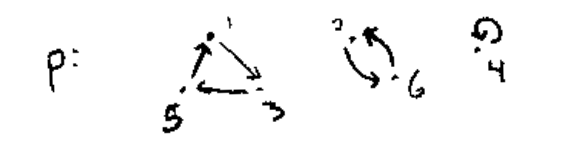
\includegraphics[scale=0.5]{images/cycle_notation}
\caption{Cycle notation describing the permutation $p$.}
\end{figure}

In our previous notation, there is some ambiguity:
\begin{align*}
p 	&= (1\;3\;5)(2\;6)(4)\\
	&= (5\;1\;3)(2\;6)(4)\\
	&= (5\;1\;3)(2\;6)\\
	&= (2\;6)(5\;1\;3).
\end{align*}

Any permutation can be written uniquely as a product of disjoint cycles, up to reordering cycles, cyclically permuting elements in a cycle, and dropping $1$-cycles. Notice that
$$
q = (1\;2)(3\;4\;5\;6).
$$
Therefore,
\begin{align*}
pq 	&= (2\;6)(1\;3\;5)(1\;2)(3\;4\;5\;6)\\
	&= (1\;4\;5\;2\;3\;6).
\end{align*}
Observe that 
$$
p^6 = e
$$
as disjoint cycles commute, and 
$$
p^6 = (1\;3\;5)^6(2\;6)^6(4)^6 = e\cdot e\cdot e.
$$

Now consider
\begin{align*}
q^{-1}pq	&= \left(\begin{array}{cccccc} 1 & 2&3&4&5&6\\2&1&4&5&6&3\end{array}\right)^{-1}(1\;3\;5)(2\;6)(4) \left(\begin{array}{cccccc} 1 & 2&3&4&5&6\\2&1&4&5&6&3\end{array}\right)\\
		&= (2\;4\;6)(1\;3)(5).
\end{align*}
Notice that the cycle shape stays the same under conjugation. Also, notice that each number corresponds to its $q$-image:
$$
(2\;4\;6)(1\;3)(5) = (1q\;3q\;5q)(2q\;6q)(4q).
$$
Suppose $ip = j$, i.e. $p$ maps $i$ to $j$. Then 
$$
(iq)(q^{-1}pq) = (ip)q.
$$
So, if 
$$
p = (i_1\;i_2\;\hdots\;i_r)(i_1'\;i_2'\;\hdots\;i_s')\cdots,
$$
then 
$$
q^{-1}pq = ((i_1q)\;(i_2q)\;(i_3q)\;\hdots\;(i_rq))((i_1'q)\;(i_2'q)\;(i_3'q)\;\hdots\;(i_s'q))\cdots.
$$

\begin{proposition}
Two conjugate permutations in $S_n$ have the same cycle shape, i.e. when expressed as a product of disjoint cycles, they have the same number of cycles each of the same length. Conversely, if two permutations have the same cycle shape, they are conjugate. 
\end{proposition}
Example: does 
$$
q^{-1}(1\;3\;5)(2\;6)(4)q = (6\;5\;4)(3\;2)(1)
$$
hold? Take 
$$
q = \left(\begin{array}{cccccc} 1 & 2&3&4&5&6\\6&3&5&1&4&2\end{array}\right).
$$
We can always find such a $q$.

Exercise: 
$$
\#\{ q \in S_{12} : q^{-1}(1\;2)(3\;4)(5\;6)(7\;8\;9)(10\;11\;12)q = (1\;2)(3\;4)(5\;6)(7\;8\;9)(10\;11\;12)\} = (3!)(2^3)(2!)(3^2).
$$
If $p$ has $a_1$ $1$-cycles, $a_2$ $2$-cycles, etc., then how many $q$ satisfy $q^{-1}pq=p$? We find that it is 
$$
\prod_i a_i! i^{a_i}.
$$

Take $S_5$, whose order is $120$. Its conjugacy classes consist of a five-cycle (order $4! = 24$), a four-cycle and a one-cycle (order $30$), a three-cycle and two one-cycles (order $20$), a three-cycle and a two-cycle (order $20$), two two-cycles and a one-cycle (order $15$), a two-cycle and three one-cycles (order $10$), or five one-cycles (order $1$). The number of conjugacy classes of $p$ is  
$$
n! / \prod_i a_i! i^{a_i}
$$
with the construction above. 

Exercise: for $p$ prime, what is the normalizer in $S_p$ of a Sylow $p$-subgroup $P$?

\section{The simplicity of $A_5$, rings, ideals} 
\begin{proposition}
$[G:H] = 2\implies H\lhd G$.
\end{proposition}
\begin{proof}
Suppose $g\in G$. If $g\in H$, then $gH = Hg$. If $g \notin H$, 
$$
gH = G \setminus H
$$
and
$$
Hg = G\setminus H.
$$
Thus, in either case,
$$
gH = Hg.
$$
\end{proof}
Let $H\subset G$ be a Sylow $p$-subgroup. Then 
\begin{enumerate}[label=(\roman*)]
\item $H$ is normal iff $n_p(G) = 1$.
\item $[G : N_G(H)] = [G : \textrm{Stab}]$, where $\textrm{Stab}$ is the stabilizer of $H$ where $G$ acts on the set of Sylow $p$-subgroups by conjugation. By the counting formula, $[G : \textrm{Stab}] = \#\{ \textrm{orbits of $H$ under this action}\}$, which is $n_p(G)$. So 
$$
[G : N_G(H)] = n_p(G).
$$
\item if $|G| = pm$ where $p$ and $m$ are coprime, then 
$$
\# \{\textrm{elements of order $p$ in $G$} \} = n_p(G)(p-1).
$$
\end{enumerate}

Groups of order $pq$ for $p < q$ prime  must have a normal Sylow $q$-subgroup ($n_q(G)=1$). If $p\nmid q-1$ then $n_p(G)=1$ and $G\simeq \Z/pq\Z$. If $p\mid q-1$ then $\exists!$ non-abelian group of order $pq$. For groups $G$ of order $12$, either $G$ has a normal Sylow $3$-subgroup or $G\simeq A_4$ (in which case $G$ has a normal $2$-Sylow).

More generally, suppose $G$ is of order $p^2q$. If $p>q$, then there must be a normal Sylow $p$-subgroup. If $p<q$, then either $G$ has a normal Sylow $q$-subgroup or $p^2q=12$ and $G\simeq A_4$. 

Elements in $S_n$ are conjugate iff they have the same cycle shape.

\begin{proposition}
$A_5$ is simple.
\end{proposition}
We will prove a converse.
\begin{proposition}
If $G$ is a simple group of order $60$, then $G \simeq A_5$.
\end{proposition}
\begin{proof}
$n_2(G)\equiv 1\pmod 2$ and $n_2(G) \mid 15$, so $n_2(G) = 3,5,15$. We use this strategy:
\begin{enumerate}[label=(\roman*)]
\item $n_2(G) \neq 3$.
\item $\exists N\subset G$ of index $5$.
\item Use the action of $G$ on the coset space $G/N$ with only even permutations. 
\end{enumerate}
We commence the proof.
\begin{enumerate}[label=(\roman*)]
\item It suffices to show that $G$ has no proper subgroups of less than index $5$ since if $P$ is a Sylow $2$-subgroup, 
$$
[G:N_G(P)] = n_2(G).
$$
Suppose $[G:H] = 2,3,\textrm{ or }4$. Then there is a transitive action of $G$ on $G/H$ by left multiplication. Every $g\in G$ induces a permutation of this coset space. The natural action of $G$ on $G/H$ gives us a homomorphism 
$$
\phi : G \to \Sym(G/H) : g\mapsto \textrm{permutation induced by $g$}. 
$$
Note 
$$
\ker\phi \subset H \subsetneq G.
$$
Moreover, $\ker \phi$ is normal, so $G$ is simple, implying $\ker\phi $ is trivial. So $\phi$ is injective (perhaps by the isomorphism theorem). Observe that
$$
G\subset \Sym(G/H) \simeq S_{[G:H]},
$$
and by hypothesis, $S_{[G:H]}$ has order $2!$, $3!$, or $4!$. $G$ is of order $60$: contradiction. 

\item $n_2(G) = 5\implies G\simeq A_5$. Let $P$ be a Sylow $2$-subgroup and $N=N_G(P)$, and notice that
$$
[G:N] = n_2(G) = 5.
$$
There is an action of $G$ on $G/N$. There is once again a homomorphism 
$$
\phi : G\to\Sym(G/N) \simeq S_5.
$$
We know that $N$ is proper, so by $\ker\phi\subset N$, $\ker \phi\neq G$, and for simplicity, $\ker \phi$ is trivial. Thus 
$$
G\subsetneq S_5.
$$
Suppose 
$$
G\not\subset A_5.
$$
So
$$
GA_5 = S_5.
$$
We get that
$$
[G:A_5\cap G] = [S_5:A_5] = 2 \implies A_5\cap G \lhd G. % confused by [G:A_5\cap G] = [S_5:A_5] 
$$
$G$ is simple: contradiction. 
$$
G\subset A_5 \land \# G = \# A_5 \implies G = A_5.
$$

\item $n_2\neq 15$. By contradiction. Suppose $n_2 = 15$. If we can show $\exists M\subset G : [G:M] =5$, then by the same argument as in the second claim (replacing $N$ with $M$), we can show that $G\simeq A_5$. But
$$
n_2(A_5) = 5:
$$
contradiction. We omit the details of constructing such an $M$. We need to show that there are Sylow $2$-subgroups $P$ and $Q$ such that $|P\cap Q|=2$ and show that $M = |N_G(P\cap Q)| = 12$.
\end{enumerate}
\end{proof}

\begin{theorem}
$A_n$ is simple for $n\geqslant 5$.
\end{theorem}
The proof on this can be done by induction. For $n \geqslant 6$, we let $G=A_n$ and suppose that $\exists A\lhd G$ non-trivial. Let $G$ act on $\{1,\hdots,n\}$ and $G_i$ be the stabilizer of $i$. Notice that
$$
G_i \simeq A_{n-1}.
$$

We claim that $\nexists \tau\in H\neq e : \tau(i) = i$ for some $i$. Thus 
$$
\tau_1(i) = \tau_2(i)\implies \tau_1=\tau_2
$$ 
since then 
$$
\tau_2^{-1}\tau_1(i) = i.
$$
\begin{proof}
Involves showing $G_j\subset H \forall j$ and 
$$
A_n = \langle G,\hdots,G_n\rangle \subset H.
$$
Contradiction.
\end{proof}

% We claim that given $\tau\in H$, only $2$-cycles can appear in disjoint cycle decomposition. We also claim that given $\tau\in H$, $\tau$ does not just have $2$-cycles in its decomposition. 

We also have the notion of \underline{rings}. Examples of rings include $\Z$, $\Z/n\Z$, $\C$, and any field. Roughly speaking, a ring $R$ is a set equipped with an addition that forms an abelian group and a multiplication, associative, with an identity. There may not be multiplicative inverses or commutativity; however, there is distributivity. A \underline{subring} $R'\subset R$ is a subset of a ring containing the additive and multiplicative identities and closed under addition (forming a subgroup) and multiplication. 

Subrings of $R =\C$ include $\R$, $\Q$, $\Z$, and the \underline{Gaussian integers}
$$
\Z[i] = \{a + bi :a,b \in \Z\}.
$$
$R$ could be all polynomials in one variable $z$ over $\C$:
$$
R = \{a_nz^n + \cdots + a_1z + a_0 : a_i\in \C\} = \C[z],
$$
or if $R$ is a commutative ring, we have the ring $R[X_1][X_2]\cdots[X_n]$ of $n$-variable polynomials with coefficients in $R$. If $R =\Z/2$, we would find that in $R[X]$,
$$
(X+1)(X+1) = X^2 + 1.
$$
The smallest ring is $R=\{0\}$ where $1=0$.
\begin{proposition}
If $R=\{0\}$ then $1\neq 0$ in $R$.
\end{proposition}
\begin{proof}
Let $a\in R$ and suppose $1=0$. Then $a = 1\cdot a$, and $a = 0\cdot a$. But $0\cdot a = (0+0)\cdot a$. So $a = 0\cdot a + 0\cdot a$. Subtracting $0\cdot a$, $0 = 0\cdot a$. Any element is the zero element. 
\end{proof}
The next smallest ring is $\Z/2$ (a field). We have rings of every size with $\Z/n\Z$. The best way to construct rings is to start with an abelian group $(A,+,0)$. Let 
$$
R = \End(A) = \{f : A\to A \textrm{ homomorphisms}\}.
$$
We define $f+g(a) = f(a) + g(a)$, $0_R(a) = 0_A$, $(-f)(a) = -(f(a))$ for addition. We define $f\times g(a) = f(g(a))$, $1(a) = a$ for multiplication. $f$ has an inverse iff it is an isomorphism of groups. 

The ring $\Z = \End(\Z, +, 0)$. Suppose 
$$
f:\Z\to\Z
$$
is a group homomorphism. We know $f(1) = n\in \Z$ determines everything, for $f(k) = k\cdot n$. Suppose $g(k) = k\cdot m $. So $f\times g(k) = f(k\cdot m) = k\cdot(m\cdot n )$: multiplication by $mn$.  If $f$ is associated to a negative number, it flips everything in $\Z$ around zero. If $g$ is also associated to a negative number, it flips everything again. Thus, the product of two negative numbers gives a positive. 
$$
\Z/n = \End(\Z/n, +, 0).
$$ 
We identify $f$ with $f(1)$, and with the approach above, we get everything else in the group. This gives a ring structure on cyclic groups. Suppose $A =(\Z/p\Z)^2$. Observe that
$$
\End(A) = M_2(\Z/p\Z).
$$
If 
$$
B = \left(\begin{array}{cc} \alpha &\beta\\\gamma&\delta\end{array}\right),
$$
then 
$$
f(a) = B \left(\begin{array}{c}a_1\\a_2\end{array}\right).
$$
This construction forms a non-commutative ring. If $A =(\Z/p\Z)^n$, 
$$
\End(A) = M_n(\Z/p\Z).
$$

A ring homomorphism
$$
f : R\to R'
$$
is a map of sets, a group homomorphism under addition, maps $1$ to $1'$, and satisfies $f(ab) = f(a)f(b)$. If $R\subset R'$, the inclusion
$$
f : R\hookrightarrow R' 
$$
is a ring homomorphism. We define 
$$
\ker f := \{a\in R : f(a) = 0_{R'}\}.
$$
Properties of $\ker f$ include that it is a subgroup under $+$. Also, if $a\in \ker f$ and $b\in R$, then $a\cdot b \in \ker f$. 

A subset $I\subset R$ which is a subgroup under $+$ and closed under $\times$ by any $b\in R$ is called an \underline{ideal}. Examples include $\ker f$ for any ring homomorphism $f$ and, given $a\in R$, 
$$
I = \{r\cdot a : r\in R\} = (a):
$$ 
the \underline{principal ideal} generated by $a$.

Any ideal $I$ is the kernel of a natural ring homomorphism 
$$
R \to R/I : a\mapsto a+I
$$ 
where $R/I$ is the \underline{quotient ring}. We define a ring structure on $R/I$ by 
$$
(a+I)(b+I) = ab + I 
$$
and
$$
(a+ I) + (b+I) = (a+b) + I.
$$

Note that the only ideals $I\subset \Z$ have the form $I=(n)$ where the quotient ring is $\Z/n\Z$. Remember that these are the only subgroups of $\Z$. Let $n\neq 0$ be the smallest positive integer in $I$. Use the Euclidean algorithm. 

Kummer: there are rings where ideals are not principal. 

A \underline{unit} in $R$ is an element $a\in R$ with a multiplicative inverse. The set of all units is denoted $R^\times$, and it forms a group under multiplication: the \underline{unit group of $R$}. If $R$ is a field, $R^\times =  R \setminus \{0\}$, but $\Z^\times = \langle \pm 1\rangle$. Note that
$$
(\Z/n\Z)^\times = \{a+n\Z : \gcd(a,n) = 1\}
$$ 
with $\varphi (n)$ elements is abelian. 

We assume commutative rings hereafter. Recall that to each ideal there is a canonical ring homomorphism $f$ with kernel $I$
$$
f : R\twoheadrightarrow R' = R/I : r\mapsto r + I
$$ 
% surjective double-headed arrow 
where $R/I$ is the quotient ring. 

Two obvious ideals in a ring $R$ are 
$$
I = \{0\} = (0) \textrm{  where  } R' = R/I = R \textrm{  and  } f = \mathrm{id}
$$
and
$$
I = R = (1) \textrm{  where  } R' = \{0\}\textrm{  and  } f(r) = 0_{R'}.
$$
These ideals are distinct iff $R$ is not the $0$-ring.
\begin{proposition}
$R$ has only two ideals $\iff R$ is a field (a ring where every non-zero element has a multiplicative inverse).
\end{proposition}
\begin{proof}
Assume $R$ is a field and that $I$ is a non-zero ideal. We want to show that $I=R$. Take $a\neq 0\in I$. Since $a$ has an inverse $r=a^{-1}\in R$, $1=a\cdot r\in I$. Since $1$ is in the ideal, for any $r\in R$, $r\cdot 1 = r\in I$. Hence $I=R$. 

Let $a\neq 0\in R$ and consider the principal ideal generated by $a$: $(a)$. $(0) \neq (a)$, so $(a)=R$. But $1\in R$, so $\exists r\in R: ra=1$, namely the multiplicative inverse of $a$. Therefore any non-zero element has a multiplicative inverse. 
\end{proof}

Take the ring $R = \Z/4\Z$. We have the trivial ideals $(0)$ and $(1) = R$. In order to get another principal ideal, we want an element without a multiplicative inverse; take $2$. We get $(2) = \{0,2\}$. If $R=\Z/n\Z$, $R$ has an ideal of order $d$ for all $d\mid n$ not necessarily distinct. If $R=\Z/p^k\Z$, we get this descending chain of ideals:
$$
(1) \supset (p) \supset (p^2) \supset \cdots\supset (p^k) = (0).
$$
$\Z$ has an infinite number of distinct ideals where all ideals
$$
I_n = (n) = (-n) = n\Z
$$
for $n\geqslant 0$ as these are the full list of subgroups and all are stable under multiplication in $\Z$. Observe 
$$
I_n \supset I_{n'} \iff n \mid n'.
$$
The lattice of ideals in $\Z$ is the lattice of nonnegative integers ordered by divisibility. Also,
$$
\Z/I_n = \Z/n\Z.
$$

Another important ring where we know all ideals is, if $F$ is a field, 
$$
R = F[X]. 
$$
We say a polynomial $p(X)\in R$ is \underline{monic} if $a_n = 1$. If $q(X)$ is any polynomial of degree $n$, $\exists! c\in F^\times: c\cdot q(X) $ is monic of degree $n$.
\begin{proposition}
Every ideal $I\subset R=F[X]$ is principal generated by the monic polynomial $f\in I$ of least degree. So ideals map bijectively to monic polynomials  and $I_f\supset I_g\iff g(X) = f(X)q(X)$ where $q$ is another polynomial in $F[X]$.
\end{proposition}
\begin{proof}
We use an analogue of the Euclidean algorithm for polynomials over a field $F$. If $f$ and $g$ are two polynomials where $\deg f \geqslant \deg g$, then $f(X)=g(X)q(X) + r(X)$ where $\deg r < \deg g$. Example: suppose $f(X) = X^3 + 2X^2+3X+7$ and $g(X) = X^2 + X +1$. So 
$$
X\cdot g(X) = X^3 +X^2 + X.
$$
Then 
$$
f(X) = X\cdot g(X) = X^2 + 2X + 7.
$$
Thus
$$
f(X) = X\cdot g(X) - g(X) = X + 6.
$$
So $g(X) = X+1$ and $r(X) = X+6$. If $I\neq 0$, take $f\in I$ of minimal degree $n$. Scale $f$ by $c = a_n^{-1}$ to make $f$ monic. This polynomial is still in the ideal. Let $h = q(X)f(X) + r(X)$ be another polynomial in $I$ where $\deg r < \deg f = n$. $q(X)f(X)\in I$. So $h(X) - q(X)f(X)\in I$. Since $r(X)\in I$, $r(X) = 0$.
\end{proof}

Consider 
$$
h : R = F[X] \to F : f(X) \mapsto f(c)
$$
where $c\in F$ fixed. $h$ is a ring homomorphism. It is an easy exercise to corroborate that
$$
h(f+g) = h(f) + h(g)
$$
and 
$$
h(f\cdot g) = h(f) h(g).
$$
There has to be a monic polynomial that generates the kernel of this. The polynomial 
$$
f(X) = X-c
$$
is monic of degree $1$ with $f(c) = 0$. So any $f\in I$ is a multiple of $X-c$.
\begin{corollary}
If $f(c) = 0$, $f(X) = (X-c)g(X)$. Over any field, a polynomial of degree $n$ has at most $n$ roots.
\end{corollary} 

Note that in $(\Z/8\Z)[X]$, $X^2-1$ has $4$ roots. 

An example of a non-principal ideal: take $R=F[X,Y]$. Consider the map 
$$
h : R\to F : f(X,Y)\mapsto f(0,0) = a_{00}.
$$
$I=\ker h$ is not generated by one element. $X,Y\in I$ and these can't both be multiples of some element other than a constant. But there are no constants in the ideal except $0$. 

For any group $G$, there is a subgroup $\{e\}\to G$. For any commutative ring $R$, there is a natural ring homomorphism $\Z\to R$ where $0\mapsto 0$ and $1\mapsto 1_R$. In general,
$$
n = \underbrace{1+ 1+\cdots + 1}_{n \textrm{ times}} \mapsto n_R = \underbrace{1_R + 1_R+\cdots +1_R}_{n \textrm{ times}}.
$$
This doesn't need to be injective. $I = \ker h =n\Z$ for some $n\geqslant 0$. Suppose $R$ is a field. Either $\ker h = (0)$ or $\ker h = p\Z$ for $p$ prime. 

\section{Properties of rings, quotient rings, integral domains, quotient fields}
If $R $ is a commutative ring, there is a ring homomorphism
$$
f : \Z\to R
$$
where $f(1) = 1_R$. The kernel is an ideal of $\Z$, so it is $n\Z$ for $n\geqslant 0$. If $R=\{0\}$, then $\ker f = \Z$. If $R= \Z,\Q,\R,\C,$ then $\ker f = \{0\}$. If $R=\Z/n\Z$, then $\ker f = n\Z$.
\begin{proposition}
If $R$ is a field, $\ker f$ is either $(0)$ or $p\Z$.
\end{proposition}
\begin{proof}
Suppose $\ker f = n\Z$ where $n$ is composite. We write $n = a\cdot b$ for $a,b>1$. Then $f(n)= 0$ in $R$ and so $f(a)\cdot f(b) = a_R \cdot b_R = 0_R$. One of $a_R$ and $b_R$ is $0$, but the kernel is multiples of $n$. Contradiction. 
\end{proof}
If $\ker f = (0)$, then the \underline{characteristic} of the field $R$ is $0$ and if $\ker f = p\Z$ then $R$ has characteristic $p$.
\begin{theorem}
(Galois) Let $F$ be a finite field. Then $|F| = p^f$ for a prime $p$.
\end{theorem}
\begin{proof}
Consider the canonical map homomorphism $\Z\to F:n\mapsto n_F$. Since $\Z$ is infinite, $\ker f\neq 0$. So $\ker f = p\Z$ and $f$ induces an injective homomorphism 
$$
\bar f : \Z/p\Z \hookrightarrow F.
$$
This gives $F$ the structure of a vector space over the field $\Z/p\Z$ which has finite dimension $f$. Then $|F| = p^f$. Also, 
$$
F \isomto (\Z/p\Z)^f
$$
as a finite-dimensional vector space.
\end{proof}
There is a unique field of order $p^f$ up to isomorphism.

\begin{proposition}
We start with a commutative ring and an ideal $R\supset I$. We get a natural surjective ring homomorphism
$$
f: R  \twoheadrightarrow R/I =\bar R 
$$
to the quotient ring. There is a bijection between ideals $I\subset J$ of $R$ containing $I$ and ideals $\bar J$ of $\bar R$ as follows:
$$
J\mapsto f(J) \subset \bar R \textrm{ and } f^{-1}(\bar J) \mapsfrom \bar J.
$$
Moreover, $R/J\isomto \bar R/\bar J$, an isomorphism of quotient rings.
\end{proposition}
\begin{proof}
% 17:00
Let's show that $f(J)\subset \bar R$. It must be closed under addition and multiplication. Suppose $f(a),f(b)\in f(J):a,b\in J$. Then $f(a) + f(b) = f(a+b)\in f(J)$ as $a+b\in J$. Suppose $f(a)\in f(J)$ and $\bar r \in \bar R$. Since $f$ is surjective, $\bar r = f(r)$, and 
$$
\bar r\cdot f(a) = f(r)\cdot f(a) = f(r\cdot a) \in f(J)
$$
because $r\cdot a\in J$. So $\bar r\cdot f(a) \in f(J)$.  \\\\
\noindent\hspace*{-23pt} \dbend\ If $f$ is not surjective, $f(J)$ need not be an ideal. For example, if you have $\Z\hookrightarrow \Q$, that is a ring homomorphism, not surjective. $f(\Z)$ is not an ideal since $\Q$ is a field and its only ideals are $(0)$ and $\Q$.\\\\
Notice that $I\subset f^{-1}(\bar J)$ as $I = f^{-1}(0)$ as $f$ has kernel $I$. $\bar J$ is an ideal so it contains $\{0\}$ and so its inverse image contains the inverse image of $0$ and so it contains $I$. It remains to show that it is an ideal. To identify the two quotients, you compose $f$ with the quotient map 
$$
\bar R \to \bar R/\bar J.
$$
What is the kernel of this composition map? Notice that the composition map is surjective because it is the composition of two surjective homomorphisms (both by quotient rings). Its kernel is the elements in $R$ such that when you map them to $R/I$ they land in $\bar J$. So that is exactly the things that are in $f^{-1}(\bar J)$, which is $J$. If you have a surjective homomorphism and you know its kernel, it identifies the quotient of $R$ by the kernel with the image, giving 
$$
R/J\isomto \bar R/\bar J.
$$
\end{proof}

$I$ is a \underline{maximal ideal} of $R$ if there are no $R$-ideals containing $I$ other than $R$ and $I$. $R/I$ is a field iff $I$ is a maximal ideal.

Suppose $a\in R$. If we want a ring $\bar R$ which is an image of $R$ where $\bar a=0$, then the largest such quotient is $\bar R = R/(a)$. If we want one where $\bar{a_1}=\bar{a_2}=\cdots=\bar{a_n}=0$, $\bar R = R/(a_1,a_2,\hdots,a_n)$ or $\bar R =  R/(a_1)/(a_2)/( a_3) \cdots$.

We now consider $R = \Z[i]$. Suppose we want $2+i = 0$. Let $I = (2+i)$ and consider $\bar R = R/I$. We want to identify $\bar R$. Identify first $I\cap \Z$. We claim that $5\in I\cap \Z$. Notice
$$
5 = (2+i)(2-i).
$$
So $I\supset 5\Z$. So $I\cap \Z$ is either $\Z$ or $5\Z$. We claim $(2+i)(a+bi)\in \Z \mid 5$. If this is true, $I\cap \Z = 5\Z$.  
$$
(2+i)(a+bi) = (2a-b) + (2b+a)i,
$$
and for this to be an integer, $a  = -2b$. We get $-5b$, which always divides $5$. So $I\cap \Z = 5\Z$. The canonical map
$$
\Z \to R/I =\bar R
$$
has kernel $5\Z$ and image $\Z/5\Z$. In fact, $\bar R\isomto \Z/5\Z$ under this map; in other words, the canonical map is surjective. We know that 
$$
i\equiv -2\pmod I
$$
and thus
$$
bi \equiv -2b\pmod I,
$$
so 
$$
a+bi \equiv a-2b\pmod I
$$
in $R/I$ is an integer. 

\begin{theorem}
(Gauss) If $p$ is prime with $p\equiv 1\pmod 4$, there is an ideal $I\subset \Z[i]=R $ with $R/I\isomto\Z/p\Z$. 
\end{theorem}
\begin{proof}
Let
$$
f:R\to R/I.
$$
If $f(i)$ has order $4$ in $(\Z/p\Z)^\times$, then $p\equiv 1\pmod 4$. Recall Wilson's theorem:
$$
(p-1)! \equiv -1\pmod p.
$$
It follows as you pair off elements with inverses modulo $p$ except for $p-1$. By the same argument,
$$
\left(\frac{p-1}{2}\right)!
$$
has order $4$ modulo $p$. We see that completing this factorial to $(p-1)!$ gives us $-1$. We find that $\left(({p-1})/{2}\right)!$ is equal to the second half that completed $(p-1)!$ as there are an even number of terms. $(p-1)!\equiv -1$ is of order $2$, so we get our number of order $4$ (cf. lecture $26$). Let 
$$
a\equiv \left(\frac{p-1}{2}\right)!.
$$
Let $I$ be the ideal generated by $p$ and $i-a$:
$$
I = (p,i-a).
$$
This does it by $I\cap \Z =p\Z$. See that
$$
(i-a)(b+ci) = (-ab-c) + (-ac + b)i
$$
results in $b = ac$, so 
$$
(i-a)(b+ci) = - c (a^2 + 1).
$$
$a^2 + 1 \mid p$ by definition of $a$, so the intersection is $p\Z$. But $\Z\to R/I$ is surjective as $i\equiv a\in\Z$ in $R/I$. So $R/I \isomto \Z/p\Z$.
\end{proof}

\begin{theorem}
(Gauss) Every $I\subset \Z[i]$ is principal.
\end{theorem}
\begin{corollary}
Since every $I$ is principal, so is this one
$$
I = (a+bi)
$$
and so 
$$
R/(a+bi) \isomto \Z/p\Z
$$
which implies that
$$
a^2 + b^2 = p.
$$
More generally, the order of the finite ring $R/(a+bi)$ is $a^2 + b^2$ where $a+bi\neq 0$.
\end{corollary}

We have the notion of relations in rings, i.e. if we want $a_1=a_2=\cdots=a_n=0$ in $R$, then we get the natural homomorphism
$$
f: R \to\bar R/(a_1,a_2,\hdots,a_n)
$$
where
$$
(a_1,a_2,\hdots,a_n) = r_1a_1 + r_2a_2 +\cdots+r_na_n,
$$
and all of these elements have become $0$ since they are in the $0$-coset. We can adjoin elements $\alpha$ to a ring $R$. If $R=\Z$ and $\alpha\in \C$, you can adjoin $\alpha$ to $R$:
$$
R' = R[\alpha] = \{ r_0 + r_1\alpha  + r_2\alpha^2 + \cdots + r_n\alpha^n : r_i\in R \},
$$
giving you the smallest subring of $\C$ containing $R$ and $\alpha$. This ring's structure depends on $\alpha$. If $\alpha\in R$, then $R' = R$. Here, $\alpha $ satisfies a monic polynomial over $R$: $x-\alpha = 0$. More generally, if $\alpha$ satisfies a monic polynomial of least degree $n$ over $R$, perhaps $x^2 + 1 = 0$, then 
$$
R' = \{ r_0+r_1\alpha + \cdots + r_{n-1}\alpha^{n-1} \textrm{ distinct, non-zero}: r_i \in R \} \isomto R^n
$$ 
as an abelian group with $n$ copies of $R$ additively. For example, $\Z[i] =\Z+\Z i$, and $i$ satisfies a polynomial of degree $2$. 

Also, $\alpha$ may not satisfy any polynomial with coefficients in $R$; in this case, $\alpha$ is \underline{transcendental} over $R$. An example is if $R=\Q$ and $\alpha = \pi$ (the circle constant). If this is the case, then all polynomials generated by $\alpha$ are distinct. So
$$
R[\alpha] = R[X]
$$
if $\alpha$ is transcendental. 

Going back to the case where $\alpha$ satisfies a monic polynomial of least degree $n$ over $R$, we find
$$
R[\alpha] \isomto R[X] / (f(X)).
$$
If we want a larger ring than $R$ containing a new element $\alpha$ satisfying a monic polynomial $f$ over $R$, we can take the ring $R' = R[X] / (f(X))$.

We could have written $\Z[i] = \Z[X] / (X^2 + 1)$.

Take $R=\Z/3 = \{0,1,2\}$. $0^2 \equiv 0$, $1^2 \equiv 1$, and $2^2 \equiv 1$. $2$ is not a square. $X^2 - 2 =f(X)$ is \underline{irreducible}:
$$
f(X) \neq g(X)h(X)\textrm{ where }\deg g, h\geqslant 1,
$$
in $\Z/3$ as there are no roots and it is quadratic. Take 
$$
R' = \Z/3[X] / (X^2-2) = \Z/3+\Z/3X,
$$ 
which has $9$ elements. We claim that this ring is a field. Take
$$
(a+bX)(a-bX) = a^2 - 2b^2 \neq 0 \textrm{ in } \Z/3 \textrm{ if } a,b\neq0
$$
because it follows 
$$
\left(\frac{a}{b}\right)^2 = 2,
$$
which is impossible. Since it is in a field, it is invertible. So 
$$
(a+bX)\left( \frac{a-bX}{a^2 - 2b^2} \right) = 1.
$$

More generally, let $F$ be a field and $f(X) $ be a monic polynomial with coefficients in $F$. Consider the ring $R = F[X]/(f(X))\isomto F^n$. 
\begin{proposition}
$R$ is a field $\iff f(X)$ is irreducible over $F$.
\end{proposition}
Note that two polynomials $f$ and $g$ of degree $n$ forming the rings $R[X]/f(X)$ and $R[X]/g(X)$ are both isomorphic to $R^n$ as groups, but not necessarily as fields. Take $f(X) = X^2+1$ and $g(X) = X^2 -2$ over $\Q$ for example.
\begin{proof}
$R$ has two ideals if it is a field: $(0)$ and $R$. Equivalently, $R$ is a field iff it has exactly $2$ ideals in $F[X]$ containing $I = (f(X))$, namely $I$ and $F[X]$. This follows iff $(f(X))$ is a maximal ideal of $F[X]$. But in $F[X]$ we know all ideals $I$: $(g(X))$ by the Euclidean algorithm for polynomials. But $(f(X))\subset(g(X))\subset F[X]$ iff $g(X) \mid f(X)$. Therefore, $(f(X))$ is maximal and we get an ideal containing $f(X)$ precisely when we can find a monic polynomial that divides $f(X)$. If $f$ is irreducible, only $f$ and $1$ divide it. Conversely, if this is a field, then any ideal squeezed between $(f(X))$ and $F[X]$ has to be one of the two. In the $(f(X))$ case $g(X) = f(X)$ and in the other case $g(X) = 1$.
\end{proof}

To produce a field $F'$ of order $p^2$, we need an irreducible quadratic polynomial $X^2+bX +c$ over $\Z/p$. In $p=2$, take $f(X) = X^2+X+1$; it is irreducible since there are no roots in $\Z/2$. So 
$$
F_4 = \Z/2[X]/(X^2+X+1).
$$
If $p>2$, take $X^2 -c$. It will be irreducible if $c$ is not a square in $\Z/p\Z$. 

Euler's argument that some $c\in\Z/p$ is not a square. $(\Z/p)^\times$ is an abelian group of order $p-1$. Consider the map
$$ 
h : (\Z/p)^\times \to (\Z/p)^\times
$$
where $h(a) = a^2$. This is a group homomorphism since we are in an abelian group. This homomorphism is not surjective if there is a non-square. $h$ is not surjective, so there are non-squares $c$. It is surjective iff $\ker h = \{1\}$. But 
$$
\ker h = a \in (\Z/p)^\times : a^2 \equiv 1\pmod p = \{\pm 1\}.
$$ 
So $\im h$ is of order $(p-1)/2$. Half are non-squares. 

A commutative ring is an \underline{integral domain} or domain if it has the property that if $a\cdot b = 0$ in $R$ then either $a=0$ or $b=0$ in $R$. Examples include fields. Suppose $a\cdot b=0$ and $a\neq 0$. Multiply by $a^{-1}$ to see $b=0$. $R=\Z$ is a domain and $\Z/4\Z$ is not a domain as $2\not\equiv 0\pmod 4$ but $2\cdot 2\equiv 0\pmod 4$. $R=F[X]$ is a domain. If $R$ is a domain, so is $R[X]$, and so is $R[X_1,X_2]$. If $a\cdot b= a\cdot c$ in $R$ and $a\neq 0$ then $b=c$ in $R$. 

$\Z[i]$ is a domain. If $R\hookrightarrow F$ then $R$ is a domain. 
\begin{theorem}
If $R$ is a domain there is a field $F$ we can construct from $R$ (a \underline{quotient field}) and an inclusion of rings $R\hookrightarrow F$. 
\end{theorem}
If $R=\Z$, then $F=\Q$. If $R=\Z[i]$, then $F = \Q[i]$. If $R=k[X]$ where $k$ is a field, 
$$
F=  k(X) = \{\textrm{rational functions } f(x)/g(x) : g(x) \neq 0\}.
$$
The idea behind $9.8$ is formally inverting all non-zero elements: add elements $1/a$ for all $a\neq 0$ in $R$ such that $a\cdot 1/a = 1$. Notice that if $1/6\in F$ for $R=\Z$ and $1/3\in F$, $2\cdot1/6$ gives $1/3$.
\begin{proof}
Construction of $F$ from $R$. Start with 
$$
S = \{  a/b : a\in R, b\neq0 \textrm{ in } R  \}.
$$
We introduce the equivalence relation on $S$ 
$$
a/b \sim a'/b' \iff ab' = ba' \textrm{ in } R.
$$
This is an equivalence relation since if $a''/b''$ also satisfies the above relation, then 
$$
a'b'' = b'a''.
$$
So $ab'b'' = ba'b''$ and $a'bb'' = bb'a''$. Thus
$$
ab'b'' = bb'a'' ,
$$
and then we cancel $b'$ so that $ab'' = ba''$. It is a domain, after all. This means that it is transitive and thus an equivalence relation. We define 
$$
F = S/\sim.
$$
We show that this is a field containing the domain $R$. We define addition 
$$
a/b + c/d = \frac{ad+bc}{bd},
$$
multiplication
$$
a/b \times c/d =\frac{ac}{bd},
$$
and inverses
$$
(a/b)^{-1} = b/a
$$
if $a\neq 0$. Note that
$$
R\hookrightarrow F : a\mapsto a/1.
$$
It is easy to check that if 
$$
a/b\sim a'/b' \textrm { and } c/d \sim c'/d'
$$
then
$$
\frac{ad+bc}{bd}\sim \frac{a'd'+b'c'}{b'd'},
$$
etc. 
\end{proof}

The universal property of quotient fields. If $R\hookrightarrow k$ is any ring inclusion into a field and $R\hookrightarrow F$ where $F$ is the quotient field, a natural injective homomorphism of fields $h^*$ arises from $F$ to $k$:
$$
\begin{tikzcd}[]
R \arrow[hookrightarrow]{dr} \arrow[hookrightarrow]{rr}{h}
& & k \\
& F\arrow[hookrightarrow]{ur}{h^*} 
\end{tikzcd}
$$
Note that a homomorphism of fields is always injective as the kernel must be $(0)$ or $(1)$, but $1$ can't be in the kernel since $1\mapsto 1$.
\begin{proof}
\textit{Of universal property}. Refer to the commutative diagram above. 
$$
h^*(a/b) = h(a)h(b)^{-1}
$$
and $b\neq 0$, so $h(b)^{-1}$ exists in $k$.
\end{proof}

Also note \href{https://en.wikipedia.org/wiki/Eisenstein\%27s_criterion}{Eisenstein's criterion}. Let 
$$
q(X) = a_nX^n + a_{n-1}X^{n-1} + \cdots + a_1X + a_0 \in \Z[X].
$$
If there is a prime number $p$ for which
\begin{enumerate}[label=(\roman*)]
\item $p$ divides each coefficient of $q$ except for $a_n$ and
\item $p^2$ does not divide $a_0$,
\end{enumerate}
then $q$ is irreducible over the rationals.

\section{Euclidean domains, principal ideal domains, Gaussian integers}
From now on, we will suppose $R$ is an integral domain, namely that if $a\cdot b=0$ in $R$, then either $a=0$ or $b=0$ in $R$. Examples of domains include $\Z$, $F[X]$, $R[X]$ for $R$ a domain. Non-examples include $\Z/4$ and $\Z\times \Z$. We thus define the field of fractions $F$, the smallest field that can contain $R$. We define 
$$
F = \{ a/b : b\neq 0, a\in R  \}/\sim
$$
which satisfies an equivalence relation. $R\hookrightarrow F : a\mapsto a/1$ which has an inverse $1/a$ for non-zero $a$. 

Factorization in $R=\Z$. The Euclidean algorithm says that if $|a| < |b| \in \Z$ then $b = ma + r$ where $0\leqslant r < |a|$. Every ideal $I\neq 0$ is principal generated by the smallest positive integer $d\in I$. Ideals generated by two elements $I = (a,b) = (d)$ where $d = ma + mb$, so $d = \gcd(a,b)$. If $p$ prime and $p\mid ab$, then either $p\mid a$ or $p\mid b$.
\begin{proof}
If $p\nmid a$, then $\gcd(a,p)=1$. So $1=ma+mp$, and $b = mab +mbp$. Since $p\mid ab$, $p$ divides this sum and so $b$ is divisible by $p$.
\end{proof}
Also, every integer $n$ has a unique factorization into primes.  The unit group $R^\times = \Z^\times =\langle \pm 1\rangle$.

Another ring $R$ with a Euclidean algorithm is $R=F[X]$ for $F$ a field. $g(X) = f(X) q(X) +r(X)$ where $\deg r < \deg f$. Every ideal is principal generated by $d(X)$ of least degree in $I$. Any two polynomials $f$ and $g$ have a greatest common divisor: $(d) = (f,g) = I$ where 
$$
d = m(X)f(X) + n(X)g(X).
$$ 
We say $p(X)$ is a prime polynomial (irreducible) if any factorization $p(X) = p_1(X)p_2(X)$ has $\deg p_1  = 0$. If 
$$
p(X) \mid a(X)b(X)
$$
then
$$
p(X) \mid a(X) \textrm{ or } p(X) \mid b(X).
$$
This is the same argument for $\Z$. Any $f(X) = c \cdot p_1(X)\cdots p_k(X)$ has a unique factorization into primes (irreducible polynomials). Here, the unit group $R^\times = F^\times $ is all non-zero degree-zero polynomials.

A domain $R$ is a \underline{Euclidean domain} iff $R$ has a size function 
$$
\delta : R \setminus \{0\} \to \Z_+
$$
such that for any $a,b\neq 0$ in $R$, we have $b=ma +r$ with either $r=0$ or $\delta(r) < \delta(a)$. The size function in the integers is $\delta(a) = |a|$. For polynomials, $\delta(f) = \deg(f) + 1$. In particular, if $\delta r = 1$, $r$ is a unit. 

Gauss: the ring $\Z[i]$ is Euclidean with size function
$$
\delta(a+bi) = a^2 + b^2 = |a+bi|^2.
$$
\begin{corollary}
Every ideal $I\subset \Z[i]$ is principal, so in particular, the ideal 
$$
\Z[i]/I \isomto \Z/p\Z
$$ 
where $p\equiv 1\pmod 4$ is generated by a single element $a+bi$. Fermat: 
$$
a^2 + b^2 = p.
$$
\end{corollary}

If $B, A\in \Z[i]$, we write $B = A\cdot w$ where 
$$
w=\alpha + \beta i, \alpha,\beta\in\Q.
$$ 
This follows since $B/A = B\bar A / A\bar A$, and $A\bar A$ is some positive integer. Write $\alpha = \alpha_0 + r_0$ and $\beta = \beta_0 + s_0$ where $-1/2\leqslant r_0,s_0 <1/2$ and $\alpha_0,\beta_0\in \Z$. We then get 
$$
B = A  (\alpha_0+\beta_0 i) + A(r_0 + s_0i) = AM + AR.
$$
We claim that $\delta R \leqslant 1/2\delta A$ or $R=0$. 
$$
\delta R = \delta (A)(r_0^2+s_0^2),
$$
This expression is clearly less than or equal to $\delta (A)(1/4+1/4) = 1/2\delta A$. So it holds and $\Z[i]$ is Euclidean.

This proof does not work for all rings. Consider 
$$
R = \left\{ a + b \sqrt{-5} : a,b\in \Z\right\}.
$$
We could take
$$
\delta\left(a + b\sqrt{-5}\right) = a^2 + 5b^2.
$$ 
This fails with the previously-utilized division, as instead of $\delta R = \delta (A)(r_0^2 + s_0^2)$, we get $\delta R = \delta (A)(r_0^2 + 5s_0^2)$, and this is no longer less than one. This doesn't work (in Gauss' proof). In fact, $R$ is not Euclidean for any choice of $\delta$. This follows as the number $6$ in $R$ has two distinct factorizations: $6 = 2\cdot 3 = \left( 1+\sqrt{-5} \right)\left( 1 - \sqrt{-5}\right)$. These are ``primes'' in $R$. Moreover, there are non-principal ideals; take for example $I = \left( 2, 1+\sqrt{-5} \right)$. 
$$
R/I \isom \Z/2 : a+b\sqrt{-5} \mapsto a + b \pmod 2.
$$

We have shown that if a domain $R$ is Euclidean, then $R$ is a \underline{principal ideal domain} (PID): every $I$ is principal. If this is the case, then elements $R$ have a unique factorization into prime elements. 

We should rethink ``divide,'' ``prime'' in terms of ideals. We say 
$$
a\mid b\iff b = ma, m\in R\iff b\in (a) \iff (b) \subset (a).
$$
We say $a$ divides $b$ properly if neither $a$ nor $m$ is a unit in $R$. This means 
$$
(b) \subsetneq (a) \subsetneq R.
$$
$p$ is a prime or irreducible in $R$ if $p$ is not a unit and $p$ has no proper factor in $R$. Expressed in terms of ideals,
$$
(p) \subsetneq R \iff R/(p) \textrm{ is an integral domain},
$$
and $(p)$ is a maximal principal ideal. If $R$ is a PID, this means
$$
p \textrm{ is prime} \iff (p) \textrm{ is a maximal ideal} \iff R/(p) \textrm{ is a field}.
$$

Consider $R = \Z[X]$. Take $I = (X)$. In fact, 
$$
R/I \isom \Z : f(X)\mapsto f(0).
$$
This is an integral domain. This shows that $X$ is prime in $R$, but it also shows that $R$ is not a PID, as $R/I$ is not a field. $\Z\supset 2\Z$, so there are (non-principal) ideals containing this principal ideal in $R$. From that example, we get a larger ideal $R\supsetneq J=(X,2)$ where 
$$
R\to R/J : f\mapsto f(0)\pmod 2.
$$
This is not a principal ideal. 

We get the following chain of implications:\\

{\centering
$R$ is a Euclidean domain.\\
$\Downarrow$\\
Every ideal $I\subset R$ is principal generated by an element of minimum size. \\
$\Downarrow$\\
Every element in $R$ has a unique prime factorization:
$$
a = \mathrm{unit}\cdot p_1\cdots p_r
$$
where the $p_i$s are primes in $R$ unique up to order. \par}

If $R/(p)$ is not a field, then 
$$
\exists I : (p) \subsetneq I \subsetneq R
$$
and so $I$ is not principal.

In fact, even though $\Z[X]$ is not a PID, it has unique factorization. If $R$ is a domain with unique factorization into primes, so is $R[X]$. Notice that 
$$
f(X) \in \Z[X]\subset \Q[X].
$$
We write 
$$
f(X) = c\cdot p_1(X)\cdots p_k(X)
$$
as a factorization in $\Q[X]$ where $c$ is a unit in the rationals and the $p_i$s are irreducible polynomials in $\Q[X]$. $\Q[X]$ is a PID and so it has unique factorization. Suppose $f(X) =2X + 1$. Its factorization would be
$$
f(X) = 2(X+1/2).
$$
The problem is that these factors need not be in $\Z[X]$. The analogue of a monic polynomial in $\Z[X]$ is a \underline{primitive polynomial}:
$$
f_0 = a_nX^n +\cdots + a_1X + a_0
$$
where $a_i \in\Z$ and $\gcd(a_n,\hdots,a_1,a_0) =1$. Equivalently, $(a_n,\hdots,a_1,a_0) = \Z$. We also assume that $a_n > 0$. Then any $f\in \Z[X] = c\cdot f_0$ uniquely, where $c\in\Z$ and $f_0$ is primitive in $\Z[X]$.

Moreover, if $f\in\Q[X]$, then 
$$
f = c\cdot f_0
$$
is unique, where $c\in\Q^\times$ and $f_0$ is primitive in $\Z[X]$. We can multiply $f$ by a large integer $N$ such that $Na_i\in \Z$ for all $i$ so
$$
N\cdot f(X)\in \Z[X].
$$ 
We write the above uniquely as $d\cdot f_0$ where $d\in\Z$ and $f_0$ is primitive. We then write  
$$
f = (d/N)f_0. 
$$
It is easy to prove unicity. Note that, with the notation used heretofore,
$$
f(X)\in\Z[X] \iff c\in \Z.
$$
$c$ is called the \underline{content} of $f$.

Let us return to our factorization of $f$ in $\Q[X]$:
$$
f(X) = c\cdot p_1(X)\cdots p_k(X).
$$
We write 
$$
f(X) = c\cdot c_1q_1(X) \cdot c_2q_2(X)\cdots c_kq_k(X).
$$
Further,
$$
f(X) = d\cdot q_1(X)\cdots q_k(X).
$$
Each of the $q_i$s is irreducible in $\Z[X]$ and $d = c\cdot c_1\cdots c_k\in\Q^\times$.
\begin{lemma}
(Gauss' lemma) If $f_0$ and $g_0$ are primitive, so is their product.
\end{lemma}
\begin{proof}
If not, say the prime $p$ divides all the coefficients of $f_0(X)g_0(X)$. Consider the ring homomorphism
$$
\Z[X] \to \Z/p\Z[X] : a\mapsto a \pmod p : X\mapsto X : \sum a_nX^n \mapsto \sum \bar{ a_n} X^n
$$
where the leading coefficient is not divisible by $p$. Then the image of this polynomial under the homomorphism is $0$:
$$
f_0(X)g_0(X) = 0.
$$
So
$$
\bar{f_0(X)}\cdot\bar{g_0(X)} = 0.
$$
But $\Z/p[X]$ is an integral domain. So either $\bar{f_0(X)} = 0$ or $\bar{g_0(X)}=0$. Contradiction on primitivity. 
\end{proof}
\begin{proof} % https://en.wikipedia.org/wiki/Gauss%27s_lemma_(polynomials)#Proofs_of_the_primitivity_statement
Clearly the product $f_0 g_0$ of two primitive polynomials has integer coefficients. Therefore, if it is not primitive, there must be a prime $p$ which is a common divisor of all its coefficients. But $p$ can not divide all the coefficients of either $f_0$ or $g_0$ (otherwise they would not be primitive). Let $a_rX^r$ be the first term of $f_0$ not divisible by $p$ and let $b_sX^s$ be the first term of $g_0$ not divisible by $p$. Now consider the term $X^{r + s}$ in the product. Its coefficient must take the following form:
$$
a_{r}b_{s}+a_{r+1}b_{s-1}+a_{r+2}b_{s-2}+\cdots +a_{r-1}b_{s+1}+a_{r-2}b_{s+2}+\cdots.
$$
The first term is not divisible by $p$ (because $p$ is prime), yet all the remaining ones are, so the entire sum cannot be divisible by $p$. By assumption all coefficients in the product are divisible by $p$. Therefore, the coefficients of the product can have no common divisor and are thus primitive.
\end{proof}
From this lemma it follows that $q_1\cdots q_k$ is primitive and so its content is $1$. Therefore the content of $f$ is $d$; however $f\in\Z[X]$ so $d\in\Z$. Factoring $d$,
$$
f(X) = \pm \ell_1\ell_2\cdots \ell_s \cdot q_1(X)\cdots q_k(X).
$$
So we get that there is a unique factorization (unicity is, once again, straightforward to corroborate) of a polynomial in $\Z[X]$ into integer primes and primitive irreducible polynomials in $\Z[X]$. It is easier to prove polynomials in $\Z[X]$ are irreducible than in $\Q[X]$ as you can check irreducibility easier in $\Z/p[X]$; if a polynomial is irreducible in $\Z/p[X]$, it is irreducible in $\Z[X]$. $p$ is prime in $\Z$ but not necessarily $\Q$.

$X^3 + X + 1 =f(X)$ is irreducible.
\begin{proof}
Look at the image of $f$ in $\Z/2[X]$. Does it factor $f(X) = m(X)n(X)$? $m$ must be of degree $1$ and $n$ must be of degree $2$. So 
$$
f = (X+a)(X^2+bX+c).
$$
Then $f(-a) = 0$ in $\Z/2$. There is no element in $\Z/2$ satisfying that, so there is no factorization. 
\end{proof}
\noindent\hspace*{-23pt} \dbend\ There are polynomials in $\Z[X]$ that are irreducible but reducible mod $p$ for every prime $p$.

There is an irreducible polynomial of any degree over $\Z/2$.

Consider again the Gaussian integers, a Euclidean ring with respect to
$$
\delta(a+bi) = a^2 + b^2 = (a+bi)(a-bi).
$$
If $\alpha,\beta\in \Z[i] = R$,
$$
\beta = q\cdot\alpha + r
$$
where $\delta r < \delta \alpha$. Every ideal $I\subset \Z[i]$ is principal generated by $\alpha$ with $\delta\alpha$ minimal. If $I\neq (0)$, then $R/I$ is a finite ring, i.e. $I$ has finite index in $R$.
\begin{proof}
Assume $\alpha\neq 0 \in I$. Then
$$
\alpha\bar\alpha = n>0\in I.
$$
Therefore, $R\supset I\supset (n)$ has finite index $n^2$ because 
$$
(n) = \{ na+nbi : a,b\in \Z\},
$$
and so 
$$
R/(n) = \{a+bi : 0\leqslant a,b < n\},
$$
giving us $n^2$ cosets (finite).
\end{proof}

In fact, if $I=(\alpha)$, then 
$$
\# (R/I) = \delta\alpha = a^2+b^2.
$$ 

$R$ has unique factorization into primes:
$$
\alpha = \mathrm{unit}\cdot p_1\cdots p_r
$$
where $R/(p)$ a finite field and $(p)$ is maximal ideal. Recall that in $\Z$ the units are $\langle \pm 1\rangle$ and the primes are the usual prime numbers; in $F[X]$, the units are $F^\times$, the polynomials of degree zero, and the primes are irreducible monic polynomials over $F$. 

Observe that 
$$
\delta : R\to\Z_+ : \alpha\mapsto\alpha\bar\alpha=a^2+b^2
$$
has the property that 
$$
\delta(\alpha\beta) = \delta(\alpha)\delta(\beta).
$$
We claim that $\alpha$ is a unit iff $\delta \alpha =1$.
\begin{proof}
If $\delta \alpha =1$, then $\bar\alpha$ is a multiplicative inverse of $\alpha$. If $\alpha$ is a unit, then $\alpha\cdot\beta=1$ for some $\beta\in R$, so 
$$
\delta(\alpha)\delta(\beta) = \delta(1) = 1
$$
and thus
$$
\delta \alpha = +1.
$$
\end{proof}

What elements have $\delta\alpha = 1$? If $\alpha = a=bi$, this only happens when if $a = 0$ and $b=\pm 1$ or $a=\pm 1$ and $b=0$, so 
$$
R^\times =\langle i\rangle
$$
is cyclic of order $4$. What are the primes $\pi$ of $R$? We know $R/(\pi)$ is a finite field, so 
$$
\#(R/(\pi)) = p^n
$$
for $p\in \Z$ prime and $n\geqslant 1$. Recall that there is a canonical map 
$$
\phi : \Z\to F : 1\mapsto 1_F.
$$
If $F$ is finite, there is a kernel $(n)$. So $\Z/(n)\hookrightarrow F$. If $n=a\cdot b$, then $a\cdot b \equiv 0$ in $\Z/n$, so also in $F$. Since $F$ is a domain, $n$ must be prime. The power of the prime 
$$
n = \dim_{\Z/p\Z}(F).
$$
We claim that $R/(\pi)$ has order $p$ or $p^2$ as $p=\alpha\cdot \pi$ in $R$. So 
$$
(pR)\subset(\pi R)\subset R.
$$
We have seen that this index is $\delta p = p^2$. There are two cases:
\begin{enumerate}[label=(\roman*)]
\item $R/(\pi)$ has order $p^2$. Then $(\pi) = p$, so $\pi = \mathrm{unit}\cdot p$, or $p$ itself is a prime in $R$ and $R/(p)$ is a field of order $p^2$.
\item $R/(p)$ is not a field, so there are non-trivial ideals $(\pi)$ between $(p)$ and $R$. These are generated by primes with $R/(\pi)\isomto \Z/p\Z$.
\end{enumerate}
To each prime $\pi\in\Z[i]$ we can associate a rational prime $p$ and every rational prime occurs. It all comes down to whether $R/(p)$ is a field. So we study $R/(p)$ for a rational prime $p$. Observe that 
\begin{align*}
\Z[i]/(p) 	&= (\Z[X]/(X^2+1))/(p) \\
		&= \Z[X]/(X^2+1, p) \\
		&= (\Z[X]/(p))/(X^2 + 1) \\
		&= \Z/p[X]/(X^2+1).
\end{align*}
This is field when $X^2 + 1$ is irreducible over $\Z/p$, i.e. $X^2 + 1$ has no roots over $\Z/p$. We cannot solve
$$
X^2\equiv -1\pmod p.
$$ 
Suppose $p=2$. Here,
$$
X^2 + 1 \equiv (X+1)^2\pmod 2.
$$
This has a unique root, $X\equiv -1\equiv 1$. In this case, there is a unique prime $\pi=1+i$ with $R\subset (\pi)\subset(2)$. Here, $\delta \pi=2=a^2+b^2$, so $a,b=\pm 1$. The rest of the possibilities are multiples of $\pi=1+i$ by units. The polynomial was not irreducible but there was one prime-generated ideal associated to $2$. If $p\equiv 3\pmod 4$, then $X^2+1$ is irreducible mod $p$ and $R/(p)$ is a field, so $p$ is prime. Notice that
$$
p\equiv 3\pmod 4 \implies \#(\Z/p\Z)^\times = p-1 = 2\cdot \mathrm{odd}.
$$
Also, $(\Z/p\Z)^\times$ has no elements of order $4$; the Sylow $2$-subgroup has order $2$. If $p\equiv 1\pmod 4$, then 
$$
X^2 + 1 \equiv (X-a)(X+a)\implies a^2\equiv -1\pmod p.
$$
\begin{proof}
$$
\#(\Z/p\Z)^\times = p-1 = 2^{k}\cdot \mathrm{odd}
$$ 
for $k\geqslant 2$. So the Sylow $2$-subgroup is of order $2^k$, but the only elements of order $2$ are $\pm 1\pmod p$ as if $p\mid a^2-1 = (a-1)(a+1)$. There must be elements $a$ of order $4$. 
\end{proof}
We get an ideal for each factor:
$$
\pi = (p,i-a) \textrm{ and } \pi' = (p,i+a)
$$
both primes in $R$ with 
$$
R/(\pi) \isomto\Z/p.
$$ 
These are strictly bigger than the ideals generated by $p$.

\section{Algebraic integers, Dedekind domains, class groups, fractional ideals}
Primes $p \equiv 1\pmod 4$ give rise to two primes $\pi,\pi'$ in $\Z[i]$ and primes $p \equiv 3\pmod 4$ give rise to one prime $p$. Also, 
$$
\pi\cdot\pi' = p
$$
giving Fermat's theorem if $\pi = a+bi$:
$$
a^2+b^2 = p.
$$
We now study rings $R$ analogous to $\Z[i]$. For instance $R = \Z[\sqrt{-2}]$ has size function 
$$
\delta(a+b\sqrt{-2}) = a^2 + 2b^2
$$
and is Euclidean with respect to it. Another example is $R = \Z[\sqrt{-5}]$, which has no unique factorization.

We might consider 
$$ 
\Z[\sqrt{d}] =\{a+b\sqrt d\} = \Z[X]/(X^2-d).
$$
where $d$ is not a square. This is not quite the right analogue. Consider $f(X) = X^2+X+1$, whose roots are 
$$
\alpha = \frac{-1\pm\sqrt{-3}}{2}.
$$ 
Take 
$$
R=\Z[X]/(f(X))=\Z+\Z\alpha.
$$ 
This ring contains $\Z+\Z\sqrt{-3}$. They can't be equal; in fact, $\Z+\Z\sqrt{-3}$ has index $2$ in $\Z+\Z\alpha$. They both are integral domains with field of fractions $\Q(\sqrt{-3})$. Sometimes we can enlarge these rings inside the field of fractions. $\Z+\Z\alpha$ is Euclidean but the other is not, so it is better to work with these rings.

A complex number $\alpha$ is an \underline{algebraic integer} if $\alpha$ is the root of a monic polynomial $f(X)\in\Z[X]$. Every integer is an algebraic integer. $\sqrt d$ for $d\in\Z$ is an algebraic integer, and so is
$$
\frac{-1\pm\sqrt{-3}}{2}.
$$
Suppose $\alpha$ satisfies $f(X)\in\Q[X]$ with $f$ monic and irreducible. Is $\alpha$ an algebraic integer? We claim that $\alpha$ is an algebraic integer iff the monic irreducible polynomial $f(X)$ has integral coefficients. For example, $1/2$ is not an algebraic integer. Any $\alpha\in\Q\setminus\Z$ is not an algebraic integer. 
$$
\alpha =\frac{\sqrt{2}}{3}
$$
is not an algebraic integer as it satisfies 
$$
X^2 -\frac{2}{9} = 0
$$
which is a monic, irreducible polynomial with non-integral coefficients.
\begin{proof}
Let $f_0(X)$ be the primitive polynomial over $\Z$ with $f(X) = c\cdot f_0(X)$ where $c\in\Q$ is the content. Then $f_0(\alpha) = 0$. Any $g(X)\in \Z[X]$ with $g(\alpha)=0$ has the form $g(X) = f_0(X)q(X)$ where $q(X) \in \Z[X]$. We know that $g(X) = f_0(X)q(X)$ where $q(X)$ has rational coefficients as $(f) =(f_0)$ is the full ideal of polynomials in $\Q[X]$ vanishing at $\alpha$. Write 
$$
f(X) = f_0\cdot d\cdot q_0
$$
which becomes $d\cdot(f_0\cdot q_0)$. By Gauss' lemma, the product of polynomials is primitive. So $d\in \Z$. Therefore, 
$$
q = dq_0\in\Z[X].
$$
\end{proof}

Let us determine all algebraic integers in the field $\Q(\sqrt d) = \Q +\Q\sqrt d$ where $d\in\Z$ is square-free. We know that every element of $\Z+\Z(\sqrt d)$ is an algebraic integer. Sometimes we get more. Suppose any
$$
\alpha = a+b\sqrt d
$$
satisfies the quadratic monic polynomial $(X-\alpha)(X-\alpha')$ where $\alpha' = a-b\sqrt d $ with rational coefficients. We get
$$
(X-\alpha)(X-\alpha') = X^2 = (2a)X + (a^2-db^2).
$$
So (for $b\neq 0$) $\alpha=a+b\sqrt d$ is an algebraic integer in $\Q(\sqrt d)$ iff $2a$ is an integer and $a^2 = db^2$ is an integer. If $b=0$, then $\alpha = a$ is an algebraic integer only when $a\in\Z$. There are two cases:
\begin{enumerate}[label=(\roman*)]
\item $a$ is an integer. Since $a^2-b^2d$ is an integer, $b^2d$ is an integer. This implies that $b^2$ is an integer because $d$ is square-free. So $b$ is an integer. Nothing new has been found here.
\item $a$ is in $1/2\Z\setminus\Z$, i.e. $2a - m$ is an odd integer. We get $a^2 = 1/4m^2$. So $4a^2-m^2$ is an integer so $4db^2$ is an integer. We can write $db = 1/4n$. We claim that $n$ is an odd integer as we need $4$s in the denominators of $a^2$ and $db^2$. So $b=1/2n_0$ with $n_0$ an odd integer. We know
\begin{align*}
a^2 - db^2 = 1/4m^2 - d 1/4 n_0^2 = 1/4(m^2 - dn_0^2)
\end{align*}
has to be an integer. So $m^2 - dn_0^2 \equiv 0\pmod 4$. But 
$$
m^2\equiv n_0^2 \equiv 1\pmod 4.
$$
This shows that $d\equiv 1\pmod 4$. So $a$ and $b$ have to be half integers and $d$ congruent to $1$ mod $4$.
\end{enumerate}

More simply, we have $n = 2a\in \Z$ and $a^2 - db^2\in \Z$. These imply that $m = 2b \in \Z$ and $n^2 - dm^2\in \Z$. $n^2$ and $m^2\equiv 0$ or $1 \pmod 4$. If 
$$
n^2 \equiv dm^2 \pmod 4
$$ 
and $d\equiv 2$ or $3\pmod 4$, the only solution is $n^2\equiv m^2 \equiv 0 \pmod 4$, which implies that $n\equiv m \equiv 0 \pmod 2$, and so $a,b\in \Z$. If $d\equiv 1\pmod 4$ there is also the solution 
$$
n^2\equiv m^2 \equiv 1 \pmod 4,
$$
where $a$ and $b$ are half odd integers.

So $d$ is a square-free integer. If $d\equiv 2,3\pmod 4$, then the algebraic integers in $\Q(\sqrt{d})$ form the ring $\Z+\Z\sqrt d$. If $d\equiv 1\pmod 4$, the algebraic integers in $\Q(\sqrt d)$ form the larger ring
$$
\Z+\Z\left(\frac{1+\sqrt d}{2}\right).
$$

The polynomial satisfied by $\sqrt d$ is $X^2 -d$. Its discriminant is $D  = 4d$. The polynomial satisfied by $(1+\sqrt d)/2$ is $X^2 - X + (1-4)/4$ has discriminant $D  = d$. So $D $ is not always square-free, but it has the property that 
$$
D  \equiv 0\textrm{ or } 1\pmod 4.
$$
It also has the property that it is as square-free as possible given the previous property: $2^2$ divides it, but no other square. If $D  < 0$, $R$ is an imaginary quadratic ring. If $D  > 0$, $R$ is a real quadratic ring. If $D  < 0$, it can be $-3$, $-4$, $-7$, $-8$, $-11$, $-15$, $-19$, $-20$, $-23$, etc. When $D = -4$, $d=-1$ and $R$ is the Gaussian integers. If $D  > 0$, it can be $5$, $8$, $12$, $13$, $17$, $21$, $24$, $27$, $28$, etc. For every one of these numbers, we get a ring. Gauss guessed that $D  = -3$, $-4$, $-7$, $-8$, $-11$, $-19$, $-43$, $-67$, and $-163$ give a ring where every ideal is principal. Gauss guessed that for positive $D $ there are an infinite number that give this property. This guess has yet to be proven. We focus herein on $D <0$. If $D <0$, $R^\times $ is a finite, cyclic group where if $D  = -3$ it is of order $6$, if $D  = -4$ it is of order $4$, and if $D  < -4$ it is of order $2$ where $R^\times =\Z^\times = \langle \pm 1\rangle$. If $D  > 0$, $R^\times$ is always infinite. 

We write the ring of algebraic integers 
$$
R_D = \Z+\Z\left(\frac{D+\sqrt D}{2}\right).
$$
Consider the \underline{norm map}
$$
\N : R\to\Z : a+b\sqrt d\mapsto a^2-db^2.
$$
If $a+b\sqrt d=\alpha$, the map $\N$ has the effect of multiplying $\alpha$ by its conjugate $\alpha'$. This map is multiplicative:
$$
\N(\alpha\beta) = \N(\alpha)\N(\beta).
$$
Notice that since $D<0$ this will always result in a non-negative norm. 
\begin{proposition}
$\alpha$ is a unit in $R\iff\N(\alpha) = \pm 1$ is a unit in $\Z$.
\end{proposition}
\begin{proof}
If $\alpha$ is a unit, $\exists\beta\in R : \alpha\beta =1$. Then 
$$
\N(\alpha\beta) = \N(\alpha)\N(\beta) = \N(1) = 1.
$$
If $\N(\alpha) =\alpha\alpha' = \pm 1$, then $\pm\alpha'$ is an inverse for $\alpha$ since $\alpha\alpha' = \N(\alpha)$.
\end{proof}
\begin{corollary}
If $D<0$, then $\alpha $ is a unit $\iff \N(\alpha) = +1$.
\end{corollary}
Reiterating, if $D  = -3$ there are $6$ units, if $D  = -4$ there are $4$ units, and if $D  < -4$ there are $2$ units where $R^\times =\Z^\times = \langle \pm 1\rangle$.
\begin{proof}
A unit $\alpha=a+b\sqrt d$ is a solution to 
$$
a^2 - db^2 = 1
$$
where $a$ and $b$ are either integers or half integers. If $b=0$, then $a^2= 1$, so $a=\pm 1$. If $b\neq 0$, then $db^2\geqslant -d/4$. It is easy to verify when $D=-3$ or $-4$.
\end{proof}

If $D=5$, 
$$
R= \Z+\Z\left(\frac{1+\sqrt 5}{2}\right).
$$
Let $\alpha = (1+\sqrt 5)/2$. Note that $\alpha\alpha ' = -1$.  So $\alpha$ is a unit with $\alpha^{-1}=-\alpha'$. Note that $\alpha^2=(3+\sqrt 5)/2$. So
$$
\N (\alpha) = -1\implies \N(\alpha^2)= 1.
$$
And $\alpha^3=(7+3\sqrt 5)/2$ is another unit with norm $-1$. You get $\alpha^n$ all distinct and increasing with $n$. So 
$$
\{\alpha^n : n\in\Z\}
$$
is an infinite subgroup of $R^\times$.

Let's get back to $R$ when $D<0$. When $d=-1$, $R = \Z[i]$ is a Euclidean ring. If $d\equiv 3\pmod 4$ and $d<-1$, then $R$ is not a \underline{unique factorization domain}. Consider the factorization of $1-d$:
$$
1-d = (1+\sqrt d)(1-\sqrt d) =2\cdot \frac{1-d}{2}.
$$
We claim that $2$ is an irreducible element (a prime) in $R$.
\begin{proof}
Suppose $2=\alpha\beta$ with neither $\alpha$ nor $\beta$ a unit. Then 
$$
\N(2) = 4= \N(\alpha)\N(\beta).
$$
So $\N(\alpha)=\N(\beta) = 2$ as they are not units. This is impossible: if $\alpha = a+b\sqrt d$ where $a,b\in\Z$, then 
$$
\N(\alpha) = a^2 - db^2\implies b=0 \because -d\geqslant 5 \implies a^2 = 2.
$$
Contradiction since $2$ is not a square and so $2$ is an irreducible element.
\end{proof}

$2$ divides $1-d$ from the factorization above, but not $1\pm\sqrt d$. Therefore, this is not a UFD. So, not every ideal $I\subset R$ is principal. %  Review from 29:00 (proof)

Although not all ideals $I\subset R$ are principal, every $I$ can be generated by $2$ elements. Either $I=(0)$ or $I$ has finite index in $R$: $R/I$ is a finite ring where $[R:I]\leqslant n^2$.
\begin{proof}
If $\alpha\neq 0$ in $I$, $\N(\alpha) = \alpha\alpha' = n>0$ is also in $I$. So $(n)\subset I\subset R$ where the index is $n^2$.
\end{proof}

$R\subset \C$ is a discrete subgroup of $(\C,+)$ stable under multiplication. $I\subset \C$ is a smaller such subgroup stable under multiplication by $R$, or equivalently by $(D+\sqrt D)/2$. Any subgroup of $R$ of finite index can be generated as a subgroup by $2$ elements. 

``Prime element'' and ``irreducible element'' are not synonyms. $p$ is a prime element means $p$ is not a unit and 
$$
p\mid ab\implies p\mid a\textrm{ or } p\mid b.
$$
An irreducible element $r$ is not a unit and $r=ab  $ implies that either $a$ or $b$ is a unit. Let $R$ be a domain. 
\begin{proposition}
If $p\neq 0$ is prime, then $p$ is irreducible.
\end{proposition}
\begin{proof}
Suppose $p=ab$. Then $p\mid ab$. Without loss of generality $p\mid a$. So $a=pc$. $p=ab=pcb$, implying that $p(1-cb) = 0$, so $1-c=0$. $c$ is an inverse for $b$, so $b$ is a unit.
\end{proof}
\noindent\hspace*{-23pt} \dbend\ The converse is false for an arbitrary domain. For example, take $R =\Z(\sqrt d)$ where $d$ is square-free. If $d<-1$ and $d\equiv 3\pmod 4$, we look at the following factorization:
$$
2\left(\frac{1-d}{2}\right) = (1-\sqrt d)(1+\sqrt d).
$$
$2$ is irreducible but $2$ is not prime as $2\mid (1-\sqrt d)(1+\sqrt d)$ and $2\nmid (1+\sqrt d)$ and $2\nmid (1-\sqrt d)$.\\\\

Observe:


{\centering 
Rings. $\Z\times \Z$ is a ring but not a domain. \\ % https://math.stackexchange.com/questions/605398/mathbbz-times-mathbbz-is-a-pid-or-not
$\bigcup$\\
Integral domains: no $0$-divisors. If $a\neq 0$ and $ab=ac$ then $b=c$. $\Z(\sqrt d)$ where $d$ is square-free, $d<-1$, and $d\equiv 3\pmod 4$ is a domain but not a UFD. \\
$\bigcup$\\
Unique factorization domains (UFD): ``unique'' means up to reordering of factorization and up to associates. $\Z[X]$ is a UFD but not a PID. \\  % https://math.stackexchange.com/questions/36169/show-that-langle-2-x-rangle-is-not-a-principal-ideal-in-mathbb-z-x
$\bigcup$\\
Principal ideal domains (PID): $I=(d)$. The ring 
$$
\Z\left(   \frac{1+\sqrt {-19}}{2}   \right)
$$
is a PID but not a Euclidean domain.\\ % http://www.maths.qmul.ac.uk/%7Eraw/MTH5100/PIDnotED.pdf 
% see also 
% http://math.berkeley.edu/%7Egbergman/grad.hndts/nonEucPID.ps
% http://www.m-hikari.com/imf/imf-2013/29-32-2013/wongIMF29-32-2013.pdf
% https://math.stackexchange.com/questions/857971/ring-of-integers-is-a-pid-but-not-a-euclidean-domain
% http://www.math.ubc.ca/%7Ereichst/423-project-pid-not-euclidean-siqi-wei.pdf
$\bigcup$\\
Euclidean domains: there is a Euclidean norm or size function $\delta$: $\forall b\neq 0\exists q,r: a = bq+r$ where $r=0$ or $\delta r < \delta b$.\\
$\bigcup$\\
Fields\\\textrm{}\\
}

\begin{proposition}
If $R$ is a UFD and $r\neq 0\in R$ then $r$ is irreducible $\iff r$ is prime. So in UFDs we sometimes interchange prime and irreducible.
\end{proposition}

Recall that $M\subsetneq R$ is maximal iff $M\subset I\subset R$ implies $I =M, R$. We say that $M$ is maximal iff $R/M$ is a field. $P\subsetneq R$  is a \underline{prime ideal} if $ab\in P$ then $a\in P$ or $b\in P$. $p$ is a prime element iff $(p)$ is a prime ideal. \begin{proof}
$p\mid \varsigma \iff \varsigma\in (p)$. Then
$$
(p\mid ab \implies p\mid a \textrm{ or } p\mid b) \iff (ab\in (p) \implies a\in(p)\textrm{ or } b\in (p)).
$$
\end{proof} 
\noindent\hspace*{-23pt} \dbend\ $P$ prime does not imply $P=(p)$ for some prime element $p$. Take 
$$
\Z[X,Y]/(X,Y)\isomto \Z
$$
where $(X,Y)$ is a prime but not principal ideal.

\begin{proposition}
$P$ is prime $\iff R/P$ is a domain. 
\end{proposition}
\begin{proof}
Suppose $xy=0$ in $R/P$ and lift $x$ and $y$ to $\tilde x$ and $\tilde y$ in $R$. $\tilde x\tilde y$ must be in the kernel, $P$, so either $\tilde x\in P$ or $\tilde y\in P$ and so $x=0$ or $y=0$. Reverse this argument for the converse. 
\end{proof}
\begin{corollary}
$M$ maximal $\implies M$ prime.
\end{corollary}
\begin{proof}
$R/M$ field $\implies R/M$ domain.
\end{proof}
\begin{corollary}
$R$ is a domain $\iff (0)$ is prime.
\end{corollary}
\begin{proof}
$R = R/(0)$.
\end{proof}

If $I,J\subset R$, we define 
$$
IJ =\left\{  \sum_{i=1}^n a_ib_i : a_i\in I, b_i\in J  \right\}
$$
where $n$ is not fixed. One can also consider this product as the set of all formal linear combinations of elements in $I$ and $J$. Notice that
$$
(a)\cdot(b) = (ab).
$$
Let $R$ be a domain with field of fractions $K\neq R$. $R$ is a \underline{Dedekind domain} if $\forall I\subset R\exists J\neq (0)\subset R:IJ=(r)$  is principal. Suppose $K = \Q(\sqrt d)$ where $d$ is a square-free integer. Then the ring of algebraic integers in $K$
$$
\Or_K  = \begin{cases}
      \Z(\sqrt d) & d\equiv 2\textrm{ or } 3\pmod 4 \\
      \Z((1+\sqrt d)/2) & d\equiv 1\pmod 4
    \end{cases}
$$
is a Dedekind domain by Artin's proposition 10.8.10.
\begin{proposition}
If $I$ is an ideal of $\Or_K$ then $I'=\{\alpha ' = a-b\sqrt d : \alpha = a+b\sqrt d \in I\}$ is an ideal satisfying 
$$
II' = (n) \textrm { where } n\in\Z.
$$
\end{proposition}
This generalizes to a field $K$ containing $\Q$ where $\dim _\Q K < \infty$. $\Or_K$ is a Dedekind domain for such $K$. 

\begin{theorem}
Suppose $R$ is a Dedekind domain and $I\subset R$ where $I\neq (0)$. $I$ can be written uniquely up to reordering as 
$$
I = P_1\cdots P_k
$$
where the $P_i$s are non-zero prime ideals. 
\end{theorem}
This gives a way of salvaging unique factorization. In $\Z(\sqrt {-5})$,
$$
6 = 2\cdot 3 = (1+\sqrt{-5})(1-\sqrt{-5}),
$$
but 
$$
(6) = (2, 1+\sqrt{-5})(2, 1-\sqrt{-5})\cdot  (3, 1+\sqrt{-5})(3, 1-\sqrt{-5})
$$
is a unique factorization into prime ideals. This theorem is often considered a definition.

\begin{theorem}
$R$ is a PID$\iff R$ is a UFD and a Dedekind domain.
\end{theorem}
\begin{proof}
\textit{One way.} PIDs are always UFDs. We multiply any ideal (which will be principal by definition) by the unit ideal to show that it is a Dedekind domain. The other direction requires that Dedekind domains are generated by at most $2$ elements.
\end{proof}

\underline{Class groups} measure how far a Dedekind domain is from being a PID. Defining the class group of a Dedekind domain $R$ requires defining this equivalence relation:
$$
I\sim J \iff \exists r\neq 0,s\neq 0\in R : rI = sJ\textrm{ and } I,J\neq(0).
$$
Let $\langle I \rangle$ denote the equivalence class of $I$: the ideal class of $I$. Let $\Cl(R)$ be the set of ideal classes of $R$ without the $0$-ideal.
\begin{proposition}
 $$
\langle I\rangle \cdot \langle J\rangle = \langle IJ\rangle
$$ 
well-defines a group structure on $\Cl(R)$.
\end{proposition}
\begin{proposition}
If $R$ is a Dedekind domain then $R$ is a PID $\iff\Cl(R)$ is the trivial group.
\end{proposition}
For example,  
$$
\Cl(\Or_{\Q(\sqrt{-5})}) = \{\langle (1)\rangle, \langle (2, 1+\sqrt{-5} )\rangle \}\isomto \Z/2\Z.
$$
To calculate $\Cl (\Or_{\Q(\sqrt d)})$ for $d<0$ for look to section $11.10$. % https://math.stackexchange.com/questions/1046496/how-to-calculate-the-ideal-class-group-of-a-quadratic-number-field
% https://en.wikipedia.org/wiki/Minkowski%27s_bound

The ring
$$
R_D = \Z + \Z\left(\frac{D + \sqrt D}{2}\right) \subseteq \C
$$
forms a lattice. We have observed that $I \neq (0) \subset R$ finite index $(R_D : I) = \N(I)\geqslant 1$. We know not all $I$ are principal. A \underline{fractional ideal} $I$ is a lattice in $\C$ (a discrete subgroup) that is stable under multiplication by $R_D$ and contained in $\Q(\sqrt D)$. If $\beta\neq 0\in\Q(\sqrt D)\setminus R$, then $I=\beta R$ is a fractional ideal. Any ideal $I$ of $R_D$ is fractional ideal.

An $R$--fractional ideal generalizes the notion of an $R$-ideal. An $R$--fractional ideal $\mathfrak{f}$ is contained in the field of fractions $K$ of $R$ and has the property that there exists a $b\in R$ such that
$$
\mathfrak{a} = b\mathfrak{f}
$$
is an $R$-ideal. In particular, elements in $\mathfrak{f}$ can be written as a fraction with a fixed denominator:
$$
\mathfrak{f} = \{ a/b : a\in\mathfrak{a} \}.
$$
The product of two fractional ideals yields another. One may also define principal fractional ideals. If $k\in K$, 
$$
(k) = kR = \{ kr : r\in R \}.
$$
% https://mathworld.wolfram.com/FractionalIdeal.html

\begin{proposition}
(Kummer, Dedekind) The fractional ideals form an infinite abelian group under multiplication with identity $R = (1)$. The principal ideals form a subgroup. The quotient group $\mathcal{C}_D$ is a finite group called the ideal class group:
$$
\Cl_D = \frac{\textrm{fractional ideals}}{\textrm{principal ideals}}.
$$
\end{proposition}
The order of the ideal class group is denoted $h_D$, the \underline{class number}. Below is a table of discriminants and corresponding class numbers.
\begin{center}
\begin{tabular}{ c|c } 
$D$ & $h_D$ \\
\hline
$-3$ & $1$ \\
\hline
$-4$ & $1$ \\
\hline
$-7$ & $1$ \\
\hline
$-8$ & $1$ \\
\hline
$-11$ & $1$ \\
\hline
$-15$ & $2$ \\
\hline
$-19$ & $1$ \\
\hline
$-20$ & $2$ \\
\hline
$-23$ & $3$ \\
\end{tabular}
\end{center}
The last time $h_D = 1$ is $D=-163$ (generates a PID). Gauss guessed  
$$
h_D \approx |D|^{1/2}.
$$
We know that $\exists c$ such that
$$
h_D < c|D|^{1/2}\log |D|
$$
and it is expected that $\exists c'$ such that
$$
c'|D|^{1/2}/\log |D| < h_D.
$$
This hypothesis is closely related to the Riemann hypothesis.

Note that if $I\subset \Q(\sqrt D)$ is a fractional ideal, then $I = \Z\alpha +\Z\beta$. Since $\alpha,\beta\in\Q(\sqrt D)$, $\exists N\geqslant 1:N\alpha,N\beta\in R$. So $(NR)I \subset R$. Every coset in $\Cl_D$ is represented by an ideal of $R_D$, not just a fractional ideal. 

(Euler) The zeta function:
$$
\zeta(s) = \sum_{n=1}^\infty \frac{1}{n^s},\ s>1.
$$
Remarkably, he observed that
\begin{align*}
\zeta(s) 	&= \prod_{p\textrm{ prime}} \left(1-\frac{1}{p^s}\right)^{-1}\\
\end{align*}
which relates beautifully to the unicity of prime factorization. It gives an easy proof of the infinitude of the primes. Euler also found that $\sum_{p\textrm{ prime}} 1/p$ is infinite.

$p$ is a rational prime in one of three cases. 
\begin{enumerate}[label=(\roman*)]
\item $pR$ can be a prime ideal with $\N(pR)=p^2$. For example, in $\Z[i]$ when $p\equiv 3\pmod 4$.
\item There are two prime ideals between $pR$ and $R$ of index $p$. For example, in $\Z[i]$ when $p\equiv 1\pmod 4$.
\item There is one prime ideal $P$ between $pR$ and $R$ with $P^2=pR$ and index $p$. For example, in $\Z[i]$ when $p =2$. This case happens finitely many times.
\end{enumerate}

(Dirichlet 1837) Euler's notion was translated into ideals:
\begin{align*}
\zeta_{R_D}(s) 	=& \sum_{\substack{I\subseteq R_D\\I\neq(0)}} \frac{1}{(\N(I))^s} \\
			=& \prod_{P \textrm{ prime ideal}} \left(1-\frac{1}{(\N(P))^s}   \right)^{-1}\\
			=& \left(\prod_{p \textrm{ in case (i)}} \left(1-\frac{1}{p^s}   \right)^{-1}\left(1+\frac{1}{p^s} \right)^{-1}\right) \\
			&\left(\prod_{p \textrm{ in case (ii)}} \left(1-\frac{1}{p^s}   \right)^{-1}\left(1-\frac{1}{p^s}   \right)^{-1} \right)\\
			&\left( \prod_{p \textrm{ in case (iii)}} \left(1-\frac{1}{p^s}   \right)^{-1}\right).
\end{align*}
Hence
\begin{align*}
L_D(s) 	&= \zeta_{R_D}(s)/\zeta(s)\\
		&= \prod_{p \textrm{ rational prime}} (1\pm p^{-s})^{-1}\\
		&= \sum_{N\geqslant 1\textrm{ prime to } D} \frac{\pm 1}{n^s}
\end{align*}
where $\mathrm{sgn}(p^{-s})$ depends on the behaviour of the prime in the ring.

For $\Z[i]$, we get
\begin{align*}
L_{-4}(s) 	&= \left(\prod_{p \equiv 1 (\bmod 4)} \left(1-\frac{1}{p^s}   \right)^{-1}\right) \left(\prod_{p \equiv 3 (\bmod 4)} \left(1+\frac{1}{p^s}   \right)^{-1}\right)\\
	&= 1 - \frac{1}{3^s} + \frac{1}{5^s} -  \frac{1}{7^s} +  \frac{1}{9^s} -  \frac{1}{11^s} +\cdots\\
	&= \sum_{n\geqslant 1} \frac{\pm 1}{(2n-1)^s}.
\end{align*}
We get 
$$
L_{-4}(1) = \pi/4,
$$
a Leibniz result. Dirichlet ideated a class number formula: 
$$
L_D(1) = \frac{2\pi}{\sqrt{|D|}} \cdot \frac{h_D}{\#R^\times}.
$$
So
\begin{align*}
L_D(1) = \pi/4 	&=  \frac{2\pi}{\sqrt 4} \cdot \frac{h_D}{4}\\	
\implies h_D	&= 1.
\end{align*}
Dirichlet saw that this was why the class numbers were growing. The goal now is to show that $L_D(1)$ is not too small as a real number. If $L(1) \approx 1$, then $h_D\sim |D|^{1/2}$. Riemann conjectured that all zeros of $\zeta$ with $0<\Re(s)<1$ have real part $1/2$. Since
$$
|1/n^s| = 1/n^{\Re(s)},
$$
if $\Re(s)>1$, then $\zeta(s)$ converges absolutely. Riemann proved that there was a pole of $\zeta$ at $1$ and that $\zeta(s) - 1/(s-1)$ has an analytic continuation to the entire plane. He noticed that the interesting behaviour of $\zeta(s)$ happened when $0<\Re(s)<1$ and that all zeros in this interval have real part $1/2$. We can apply this to $\zeta_{R_D}$ to control its size near $1$.

Dr. Dorian M. Goldfeld, a professor at Columbia, took the following approach. Siegel proved that if for a ring $R$ that if $L_D(1)$ was too small for one $D$, it was not for all others. Goldfeld suggested that we could make another series related to an elliptic curve with a high-order zero at $s=1$. He used this fact to show that $L_D(1)$ could not be too small. But finding such an elliptic curve was very difficult. Computing such series required taking derivatives of $L_D(1)$ and seeing whether they were close to zero. You cannot prove that something is zero on a computer, only that something is very, very close to zero. Gross proved a formula for the $L$-function of elliptic curves where the first two derivatives were zero in certain cases. This allowed for one to use Goldfeld's suggested method. It was proven that
$$
h_D > c\log|D|.
$$
This came as a corollary of Gross's work. Gross endeavoured to come up with formulas like Dirichlet's for the $L$-function of elliptic curves.
\end{document}

%https://math.stackexchange.com/questions/2517869/intuition-behind-kernel-is-trivial-implies-homomorphism-is-injective